%%%%%%%%%%%%%%%%%%%%%%%%%%%%%%%%%%%%%%%%%%%%%%%%%%%%%%%%%%%%%%%%%%%%%%%%%%%%%%%
%% E-RAKSHA: AGENTIC AI FOR DEEPFAKE DETECTION
%% COMPREHENSIVE ARCHITECTURE DIAGRAMS AND VISUALIZATIONS
%% LaTeX Document with TikZ Diagrams
%% 
%% E-Raksha Hackathon 2026 - Problem Statement II
%% National Cyber Challenge by eDC IIT Delhi in collaboration with CyberPeace
%% Official Pre-Summit Event of BECon'26 and AI Impact Summit'26
%%
%% Document Version: 2.0.0
%% Last Updated: December 30, 2025
%%%%%%%%%%%%%%%%%%%%%%%%%%%%%%%%%%%%%%%%%%%%%%%%%%%%%%%%%%%%%%%%%%%%%%%%%%%%%%%

\documentclass[12pt,a4paper]{article}

%% ============================================================================
%% PACKAGES
%% ============================================================================
\usepackage[utf8]{inputenc}
\usepackage[T1]{fontenc}
\usepackage{lmodern}
\usepackage[margin=1in]{geometry}
\usepackage{tikz}
\usepackage{pgfplots}
\usepackage{amsmath,amssymb,amsfonts}
\usepackage{graphicx}
\usepackage{xcolor}
\usepackage{float}
\usepackage{caption}
\usepackage{subcaption}
\usepackage{hyperref}
\usepackage{fancyhdr}
\usepackage{tcolorbox}
\usepackage{listings}
\usepackage{algorithm}
\usepackage{algorithmic}
\usepackage{booktabs}
\usepackage{multirow}
\usepackage{array}
\usepackage{longtable}

%% ============================================================================
%% TIKZ LIBRARIES
%% ============================================================================
\usetikzlibrary{
    shapes.geometric,
    shapes.symbols,
    shapes.misc,
    shapes.arrows,
    arrows.meta,
    positioning,
    calc,
    fit,
    backgrounds,
    decorations.pathreplacing,
    decorations.markings,
    decorations.pathmorphing,
    patterns,
    shadows,
    shadows.blur,
    chains,
    matrix,
    mindmap,
    trees,
    automata,
    petri,
    3d,
    perspective
}

\pgfplotsset{compat=1.18}

%% ============================================================================
%% COLOR DEFINITIONS
%% ============================================================================
% Primary Colors
\definecolor{erakshaPrimary}{RGB}{59, 130, 246}      % Blue
\definecolor{erakshaSecondary}{RGB}{139, 92, 246}    % Purple
\definecolor{erakshaAccent}{RGB}{16, 185, 129}       % Green
\definecolor{erakshaWarning}{RGB}{245, 158, 11}      % Orange
\definecolor{erakshaDanger}{RGB}{239, 68, 68}        % Red

% Model Colors
\definecolor{bgModelColor}{RGB}{59, 130, 246}        % Blue - Baseline
\definecolor{avModelColor}{RGB}{139, 92, 246}        % Purple - Audio-Visual
\definecolor{cmModelColor}{RGB}{245, 158, 11}        % Orange - Compression
\definecolor{rrModelColor}{RGB}{236, 72, 153}        % Pink - Re-recording
\definecolor{llModelColor}{RGB}{16, 185, 129}        % Green - Low-light
\definecolor{tmModelColor}{RGB}{99, 102, 241}        % Indigo - Temporal

% Layer Colors
\definecolor{convColor}{RGB}{66, 133, 244}           % Blue - Conv layers
\definecolor{bnColor}{RGB}{52, 168, 83}              % Green - BatchNorm
\definecolor{reluColor}{RGB}{251, 188, 5}            % Yellow - ReLU
\definecolor{poolColor}{RGB}{234, 67, 53}            % Red - Pooling
\definecolor{fcColor}{RGB}{155, 89, 182}             % Purple - Fully Connected
\definecolor{lstmColor}{RGB}{26, 188, 156}           % Teal - LSTM
\definecolor{dropoutColor}{RGB}{149, 165, 166}       % Gray - Dropout

% Background Colors
\definecolor{lightBg}{RGB}{248, 250, 252}
\definecolor{darkBg}{RGB}{30, 41, 59}
\definecolor{cardBg}{RGB}{255, 255, 255}

%% ============================================================================
%% TIKZ STYLES
%% ============================================================================
\tikzset{
    % Basic node styles
    basenode/.style={
        draw,
        rounded corners=3pt,
        minimum height=0.8cm,
        minimum width=2cm,
        align=center,
        font=\small
    },
    % Layer styles
    convlayer/.style={
        basenode,
        fill=convColor!20,
        draw=convColor!80,
        thick
    },
    bnlayer/.style={
        basenode,
        fill=bnColor!20,
        draw=bnColor!80,
        thick
    },
    relulayer/.style={
        basenode,
        fill=reluColor!20,
        draw=reluColor!80,
        thick
    },
    poollayer/.style={
        basenode,
        fill=poolColor!20,
        draw=poolColor!80,
        thick
    },
    fclayer/.style={
        basenode,
        fill=fcColor!20,
        draw=fcColor!80,
        thick
    },
    lstmlayer/.style={
        basenode,
        fill=lstmColor!20,
        draw=lstmColor!80,
        thick
    },
    dropoutlayer/.style={
        basenode,
        fill=dropoutColor!20,
        draw=dropoutColor!80,
        thick
    },
    % Model block styles
    modelblock/.style={
        draw,
        rounded corners=5pt,
        minimum height=1.5cm,
        minimum width=3cm,
        align=center,
        font=\small\bfseries,
        thick,
        drop shadow={shadow xshift=2pt, shadow yshift=-2pt, opacity=0.3}
    },
    bgmodel/.style={modelblock, fill=bgModelColor!20, draw=bgModelColor!80},
    avmodel/.style={modelblock, fill=avModelColor!20, draw=avModelColor!80},
    cmmodel/.style={modelblock, fill=cmModelColor!20, draw=cmModelColor!80},
    rrmodel/.style={modelblock, fill=rrModelColor!20, draw=rrModelColor!80},
    llmodel/.style={modelblock, fill=llModelColor!20, draw=llModelColor!80},
    tmmodel/.style={modelblock, fill=tmModelColor!20, draw=tmModelColor!80},
    % Process styles
    process/.style={
        draw,
        rectangle,
        rounded corners=3pt,
        minimum height=0.8cm,
        minimum width=2.5cm,
        align=center,
        fill=white,
        thick
    },
    decision/.style={
        draw,
        diamond,
        aspect=2,
        minimum width=2cm,
        minimum height=1cm,
        align=center,
        fill=erakshaWarning!20,
        thick
    },
    startstop/.style={
        draw,
        rounded rectangle,
        minimum height=0.8cm,
        minimum width=2cm,
        align=center,
        fill=erakshaPrimary!20,
        thick
    },
    % Arrow styles
    arrow/.style={
        ->,
        >=Stealth,
        thick
    },
    doublearrow/.style={
        <->,
        >=Stealth,
        thick
    },
    dashedarrow/.style={
        ->,
        >=Stealth,
        dashed,
        thick
    },
    % Container styles
    container/.style={
        draw,
        rounded corners=8pt,
        thick,
        fill=#1!5,
        draw=#1!50
    },
    % Tensor styles
    tensor/.style={
        draw,
        rectangle,
        minimum height=0.6cm,
        minimum width=1.5cm,
        align=center,
        fill=lightBg,
        font=\footnotesize\ttfamily
    },
    % State styles
    state/.style={
        draw,
        circle,
        minimum size=1.2cm,
        align=center,
        thick
    },
    % Agent node styles
    agentnode/.style={
        draw,
        rounded corners=5pt,
        minimum height=1cm,
        minimum width=2.5cm,
        align=center,
        thick,
        fill=white
    }
}

%% ============================================================================
%% DOCUMENT SETTINGS
%% ============================================================================
\hypersetup{
    colorlinks=true,
    linkcolor=erakshaPrimary,
    filecolor=erakshaSecondary,
    urlcolor=erakshaAccent,
    pdftitle={E-RAKSHA Architecture Diagrams},
    pdfauthor={Team E-Raksha},
}

\pagestyle{fancy}
\fancyhf{}
\fancyhead[L]{\textbf{E-RAKSHA} Architecture Diagrams}
\fancyhead[R]{\thepage}
\fancyfoot[C]{E-Raksha Hackathon 2026 - Problem Statement II}

%% ============================================================================
%% TITLE PAGE
%% ============================================================================
\begin{document}

\begin{titlepage}
    \centering
    \vspace*{2cm}
    
    % Logo placeholder
    
\begin{tikzpicture}
        \node[draw, circle, minimum size=3cm, fill=erakshaPrimary!20, 
              line width=2pt, draw=erakshaPrimary] (logo) {};
        \node at (logo) {\Huge\textbf{}};
    \end{tikzpicture}
    
    \vspace{1cm}
    
    {\Huge\bfseries E-RAKSHA}\\[0.5cm]
    {\Large\itshape Agentic AI for Deepfake Detection \& Authenticity Verification}\\[1cm]
    
    \rule{\textwidth}{1pt}\\[0.5cm]
    
    {\LARGE\bfseries Comprehensive Architecture Diagrams}\\[0.3cm]
    {\large Neural Networks, System Flows, and Technical Visualizations}\\[0.5cm]
    
    \rule{\textwidth}{1pt}\\[2cm]
    
    {\large E-Raksha Hackathon 2026 --- Problem Statement II}\\[0.3cm]
    {\normalsize National Cyber Challenge by eDC IIT Delhi}\\
    {\normalsize in collaboration with CyberPeace Foundation}\\[0.3cm]
    {\small Official Pre-Summit Event of BECon'26 and AI Impact Summit'26}\\[2cm]
    
    \begin{tabular}{ll}
        \textbf{Document Version:} & 2.0.0 \\
        \textbf{Last Updated:} & December 30, 2025 \\
        \textbf{Classification:} & Technical Submission \\
    \end{tabular}
    
    \vfill
    
    {\small\textit{Team E-Raksha}}
    
\end{titlepage}

%% ============================================================================
%% TABLE OF CONTENTS
%% ============================================================================
\tableofcontents
\newpage

%%%%%%%%%%%%%%%%%%%%%%%%%%%%%%%%%%%%%%%%%%%%%%%%%%%%%%%%%%%%%%%%%%%%%%%%%%%%%%%
%% SECTION 1: HIGH-LEVEL SYSTEM ARCHITECTURE
%%%%%%%%%%%%%%%%%%%%%%%%%%%%%%%%%%%%%%%%%%%%%%%%%%%%%%%%%%%%%%%%%%%%%%%%%%%%%%%
\section{High-Level System Architecture}

\subsection{Complete E-Raksha System Architecture}

\begin{figure}[H]
\centering
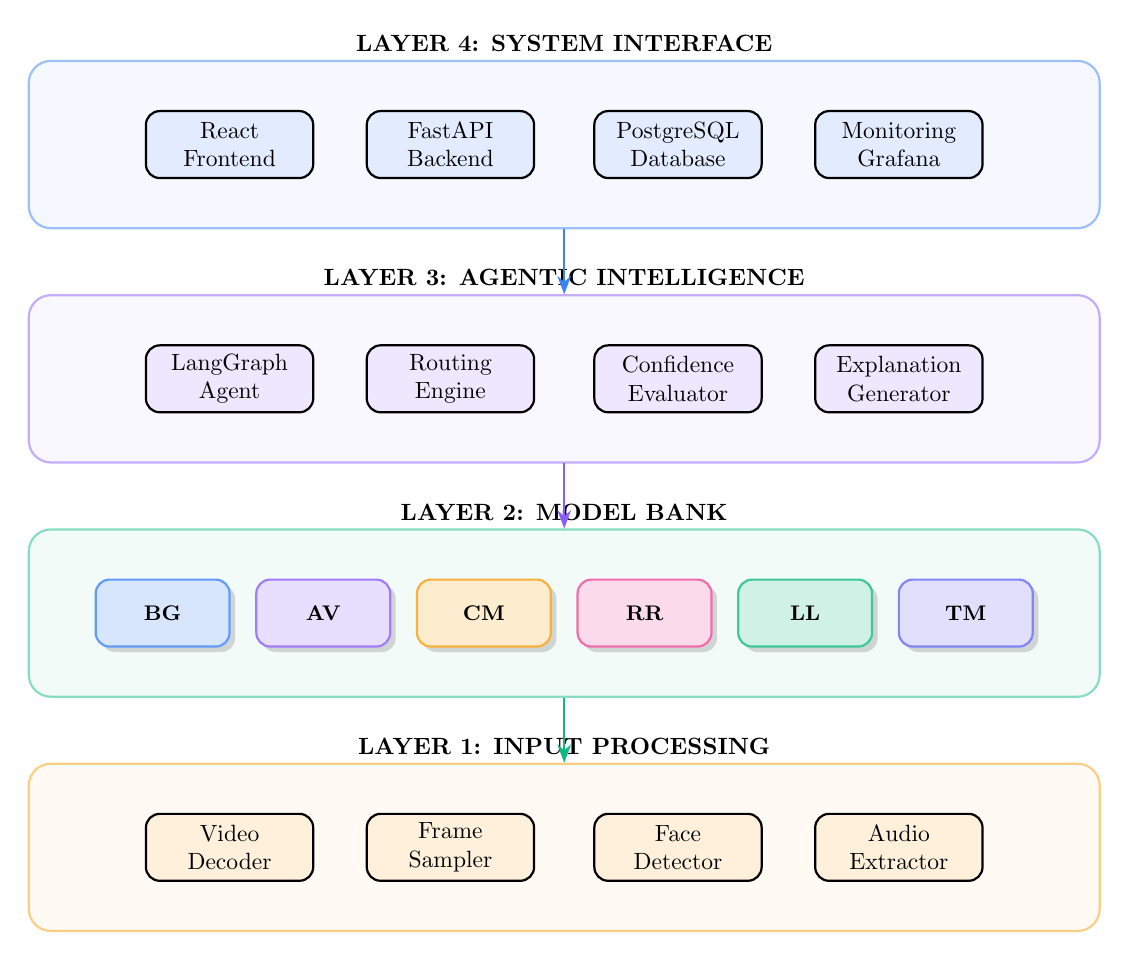
\begin{tikzpicture}[scale=0.85, transform shape]
    
    % Layer 4: System Interface
    \begin{scope}[shift={(0,9)}]
        \node[container=erakshaPrimary, minimum width=16cm, minimum height=2.5cm] (layer4) {};
        \node[above] at (layer4.north) {\textbf{LAYER 4: SYSTEM INTERFACE}};
        
        \node[agentnode, fill=erakshaPrimary!15] at (-5,0) (react) {React\\Frontend};
        \node[agentnode, fill=erakshaPrimary!15] at (-1.7,0) (fastapi) {FastAPI\\Backend};
        \node[agentnode, fill=erakshaPrimary!15] at (1.7,0) (postgres) {PostgreSQL\\Database};
        \node[agentnode, fill=erakshaPrimary!15] at (5,0) (monitor) {Monitoring\\Grafana};
    \end{scope}
    
    % Layer 3: Agentic Intelligence
    \begin{scope}[shift={(0,5.5)}]
        \node[container=erakshaSecondary, minimum width=16cm, minimum height=2.5cm] (layer3) {};
        \node[above] at (layer3.north) {\textbf{LAYER 3: AGENTIC INTELLIGENCE}};
        
        \node[agentnode, fill=erakshaSecondary!15] at (-5,0) (langgraph) {LangGraph\\Agent};
        \node[agentnode, fill=erakshaSecondary!15] at (-1.7,0) (routing) {Routing\\Engine};
        \node[agentnode, fill=erakshaSecondary!15] at (1.7,0) (confidence) {Confidence\\Evaluator};
        \node[agentnode, fill=erakshaSecondary!15] at (5,0) (explain) {Explanation\\Generator};
    \end{scope}
    
    % Layer 2: Model Bank
    \begin{scope}[shift={(0,2)}]
        \node[container=erakshaAccent, minimum width=16cm, minimum height=2.5cm] (layer2) {};
        \node[above] at (layer2.north) {\textbf{LAYER 2: MODEL BANK}};
        
        \node[bgmodel, minimum width=2cm, minimum height=1cm] at (-6,0) (bg) {BG};
        \node[avmodel, minimum width=2cm, minimum height=1cm] at (-3.6,0) (av) {AV};
        \node[cmmodel, minimum width=2cm, minimum height=1cm] at (-1.2,0) (cm) {CM};
        \node[rrmodel, minimum width=2cm, minimum height=1cm] at (1.2,0) (rr) {RR};
        \node[llmodel, minimum width=2cm, minimum height=1cm] at (3.6,0) (ll) {LL};
        \node[tmmodel, minimum width=2cm, minimum height=1cm] at (6,0) (tm) {TM};
    \end{scope}
    
    % Layer 1: Input Processing
    \begin{scope}[shift={(0,-1.5)}]
        \node[container=erakshaWarning, minimum width=16cm, minimum height=2.5cm] (layer1) {};
        \node[above] at (layer1.north) {\textbf{LAYER 1: INPUT PROCESSING}};
        
        \node[agentnode, fill=erakshaWarning!15] at (-5,0) (decoder) {Video\\Decoder};
        \node[agentnode, fill=erakshaWarning!15] at (-1.7,0) (sampler) {Frame\\Sampler};
        \node[agentnode, fill=erakshaWarning!15] at (1.7,0) (facedet) {Face\\Detector};
        \node[agentnode, fill=erakshaWarning!15] at (5,0) (audioext) {Audio\\Extractor};
    \end{scope}
    
    % Arrows between layers
    \draw[arrow, thick, erakshaPrimary] (layer4.south) -- (layer3.north);
    \draw[arrow, thick, erakshaSecondary] (layer3.south) -- (layer2.north);
    \draw[arrow, thick, erakshaAccent] (layer2.south) -- (layer1.north);
    
\end{tikzpicture}
\caption{Complete E-Raksha Four-Layer System Architecture}
\label{fig:system-architecture}
\end{figure}

\subsection{Data Flow Pipeline}

\begin{figure}[H]
\centering
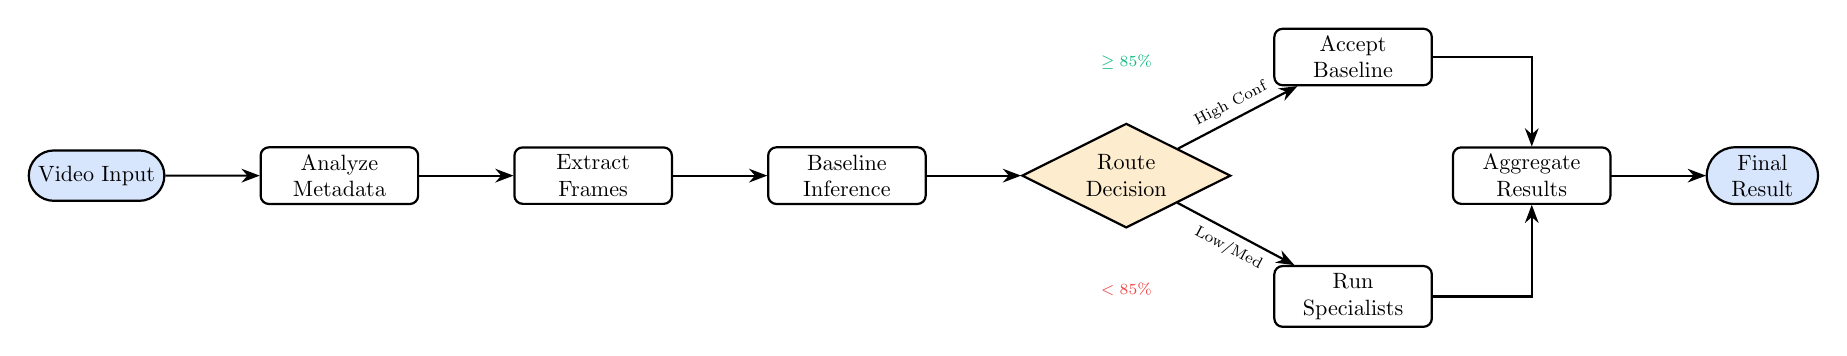
\begin{tikzpicture}[scale=0.8, transform shape, node distance=1.5cm]
    
    % Input
    \node[startstop] (input) {Video Input};
    
    % Processing chain
    \node[process, right=of input] (analyze) {Analyze\\Metadata};
    \node[process, right=of analyze] (extract) {Extract\\Frames};
    \node[process, right=of extract] (baseline) {Baseline\\Inference};
    \node[decision, right=of baseline] (route) {Route\\Decision};
    
    % High confidence path
    \node[process, above right=1cm and 1.5cm of route] (accept) {Accept\\Baseline};
    
    % Low/Medium confidence path
    \node[process, below right=1cm and 1.5cm of route] (specialists) {Run\\Specialists};
    
    % Aggregation
    \node[process, right=3.5cm of route] (aggregate) {Aggregate\\Results};
    
    % Output
    \node[startstop, right=of aggregate] (output) {Final\\Result};
    
    % Arrows
    \draw[arrow] (input) -- (analyze);
    \draw[arrow] (analyze) -- (extract);
    \draw[arrow] (extract) -- (baseline);
    \draw[arrow] (baseline) -- (route);
    
    \draw[arrow] (route) -- node[above, sloped, font=\scriptsize] {High Conf} (accept);
    \draw[arrow] (route) -- node[below, sloped, font=\scriptsize] {Low/Med} (specialists);
    
    \draw[arrow] (accept) -| (aggregate);
    \draw[arrow] (specialists) -| (aggregate);
    
    \draw[arrow] (aggregate) -- (output);
    
    % Confidence labels
    \node[font=\scriptsize, text=erakshaAccent] at ($(route)+(0,1.8)$) {$\geq 85\%$};
    \node[font=\scriptsize, text=erakshaDanger] at ($(route)+(0,-1.8)$) {$< 85\%$};
    
\end{tikzpicture}
\caption{Data Flow Pipeline with Intelligent Routing}
\label{fig:data-flow}
\end{figure}

\subsection{Component Interaction Diagram}

\begin{figure}[H]
\centering
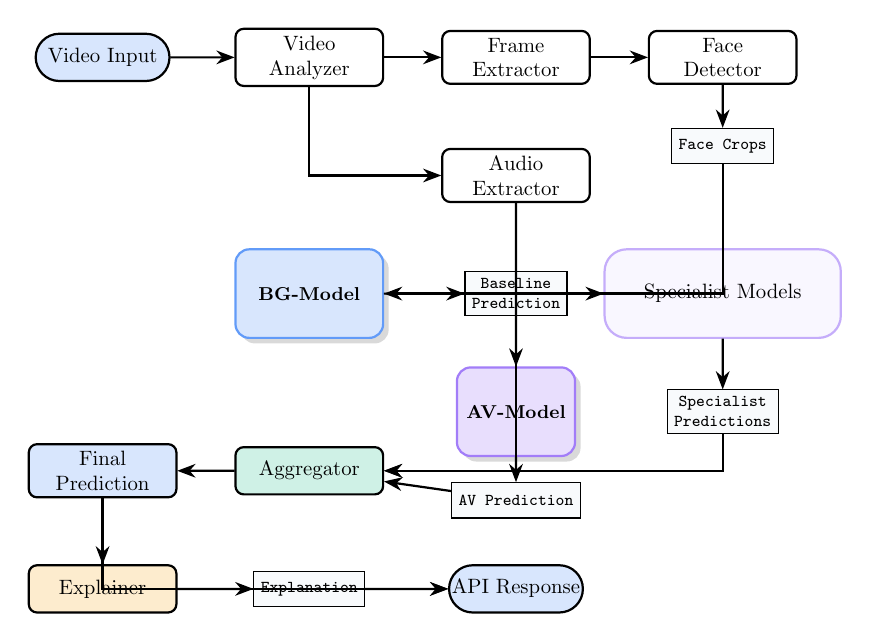
\begin{tikzpicture}[scale=0.75, transform shape]
    
    % Video Input
    \node[startstop, minimum width=2.5cm] (video) at (0,0) {Video Input};
    
    % Video Analyzer
    \node[process] (analyzer) at (3.5,0) {Video\\Analyzer};
    
    % Frame Extractor
    \node[process] (frameext) at (7,0) {Frame\\Extractor};
    
    % Audio Extractor
    \node[process] (audioext) at (7,-2) {Audio\\Extractor};
    
    % Face Detector
    \node[process] (facedet) at (10.5,0) {Face\\Detector};
    
    % Face Crops
    \node[tensor] (crops) at (10.5,-1.5) {Face Crops};
    
    % BG-Model
    \node[bgmodel, minimum width=2.5cm] (bgmodel) at (3.5,-4) {BG-Model};
    
    % Baseline Prediction
    \node[tensor] (basepred) at (7,-4) {Baseline\\Prediction};
    
    % Specialist Models
    \node[container=erakshaSecondary, minimum width=4cm, minimum height=1.5cm] (specmodels) at (10.5,-4) {};
    \node at (specmodels) {Specialist Models};
    
    % Specialist Predictions
    \node[tensor] (specpred) at (10.5,-6) {Specialist\\Predictions};
    
    % Audio to AV-Model
    \node[avmodel, minimum width=2cm] (avmodel) at (7,-6) {AV-Model};
    
    % AV Prediction
    \node[tensor] (avpred) at (7,-7.5) {AV Prediction};
    
    % Aggregator
    \node[process, fill=erakshaAccent!20] (aggregator) at (3.5,-7) {Aggregator};
    
    % Final Prediction
    \node[process, fill=erakshaPrimary!20] (finalpred) at (0,-7) {Final\\Prediction};
    
    % Explainer
    \node[process, fill=erakshaWarning!20] (explainer) at (0,-9) {Explainer};
    
    % Explanation
    \node[tensor] (explanation) at (3.5,-9) {Explanation};
    
    % API Response
    \node[startstop, minimum width=2.5cm] (response) at (7,-9) {API Response};
    
    % Arrows
    \draw[arrow] (video) -- (analyzer);
    \draw[arrow] (analyzer) -- (frameext);
    \draw[arrow] (analyzer) |- (audioext);
    \draw[arrow] (frameext) -- (facedet);
    \draw[arrow] (facedet) -- (crops);
    \draw[arrow] (crops) |- (bgmodel);
    \draw[arrow] (bgmodel) -- (basepred);
    \draw[arrow] (basepred) -- (specmodels);
    \draw[arrow] (specmodels) -- (specpred);
    \draw[arrow] (audioext) -- (avmodel);
    \draw[arrow] (avmodel) -- (avpred);
    \draw[arrow] (specpred) |- (aggregator);
    \draw[arrow] (avpred) -- (aggregator);
    \draw[arrow] (basepred) |- (aggregator);
    \draw[arrow] (aggregator) -- (finalpred);
    \draw[arrow] (finalpred) -- (explainer);
    \draw[arrow] (explainer) -- (explanation);
    \draw[arrow] (finalpred) |- (response);
    \draw[arrow] (explanation) -- (response);
    
\end{tikzpicture}
\caption{Detailed Component Interaction Diagram}
\label{fig:component-interaction}
\end{figure}

\newpage

%%%%%%%%%%%%%%%%%%%%%%%%%%%%%%%%%%%%%%%%%%%%%%%%%%%%%%%%%%%%%%%%%%%%%%%%%%%%%%%
%% SECTION 2: AGENTIC AI SYSTEM
%%%%%%%%%%%%%%%%%%%%%%%%%%%%%%%%%%%%%%%%%%%%%%%%%%%%%%%%%%%%%%%%%%%%%%%%%%%%%%%
\section{Agentic AI System Design}

\subsection{Agent State Machine}

\begin{figure}[H]
\centering
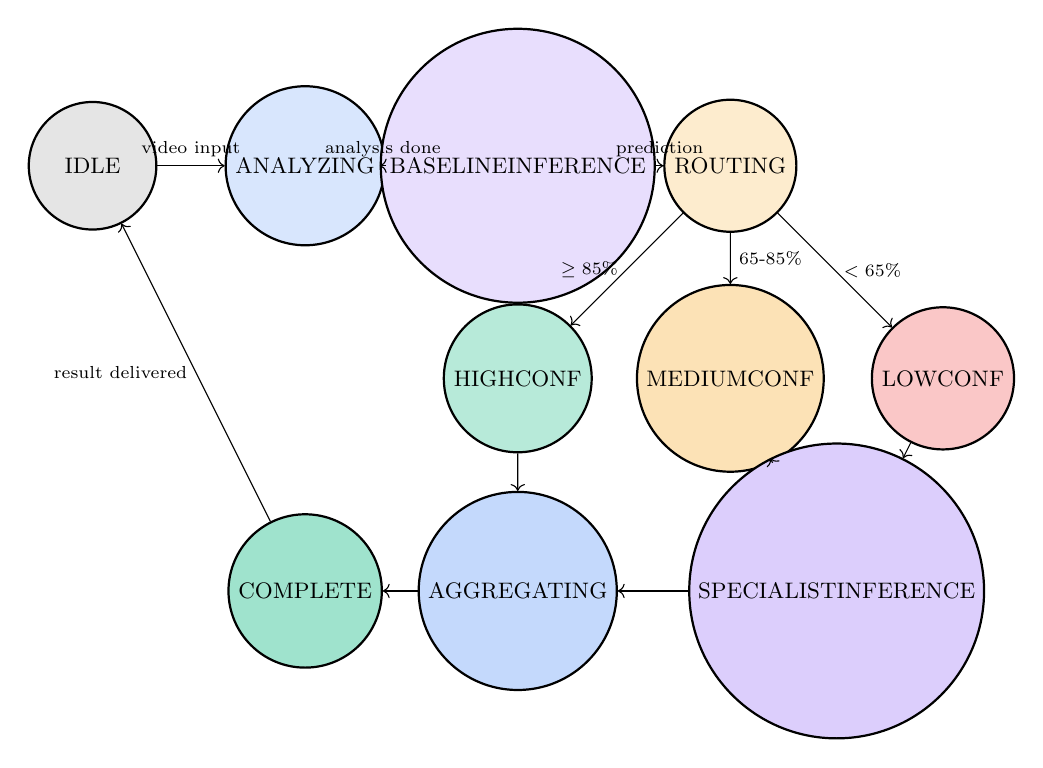
\begin{tikzpicture}[scale=0.9, transform shape, 
    state/.style={draw, circle, minimum size=1.8cm, thick, font=\small},
    every edge/.style={draw, ->, >=Stealth, thick}]
    
    % States
    \node[state, fill=gray!20] (idle) at (0,0) {IDLE};
    \node[state, fill=erakshaPrimary!20] (analyzing) at (3,0) {ANALYZING};
    \node[state, fill=erakshaSecondary!20] (baseline) at (6,0) {BASELINE\\INFERENCE};
    \node[state, fill=erakshaWarning!20] (routing) at (9,0) {ROUTING};
    
    % Confidence states
    \node[state, fill=erakshaAccent!30] (high) at (6,-3) {HIGH\\CONF};
    \node[state, fill=erakshaWarning!30] (medium) at (9,-3) {MEDIUM\\CONF};
    \node[state, fill=erakshaDanger!30] (low) at (12,-3) {LOW\\CONF};
    
    % Specialist inference
    \node[state, fill=erakshaSecondary!30] (specialist) at (10.5,-6) {SPECIALIST\\INFERENCE};
    
    % Aggregating
    \node[state, fill=erakshaPrimary!30] (aggregating) at (6,-6) {AGGREGATING};
    
    % Complete
    \node[state, fill=erakshaAccent!40] (complete) at (3,-6) {COMPLETE};
    
    % Transitions
    \draw[->] (idle) -- node[above, font=\scriptsize] {video input} (analyzing);
    \draw[->] (analyzing) -- node[above, font=\scriptsize] {analysis done} (baseline);
    \draw[->] (baseline) -- node[above, font=\scriptsize] {prediction} (routing);
    
    \draw[->] (routing) -- node[left, font=\scriptsize] {$\geq 85\%$} (high);
    \draw[->] (routing) -- node[right, font=\scriptsize] {65-85\%} (medium);
    \draw[->] (routing) -- node[right, font=\scriptsize] {$< 65\%$} (low);
    
    \draw[->] (high) -- (aggregating);
    \draw[->] (medium) -- (specialist);
    \draw[->] (low) -- (specialist);
    
    \draw[->] (specialist) -- (aggregating);
    \draw[->] (aggregating) -- (complete);
    \draw[->] (complete) -- node[left, font=\scriptsize] {result delivered} (idle);
    
\end{tikzpicture}
\caption{Agent State Machine with Confidence-Based Routing}
\label{fig:state-machine}
\end{figure}

\subsection{LangGraph Workflow}

\begin{figure}[H]
\centering
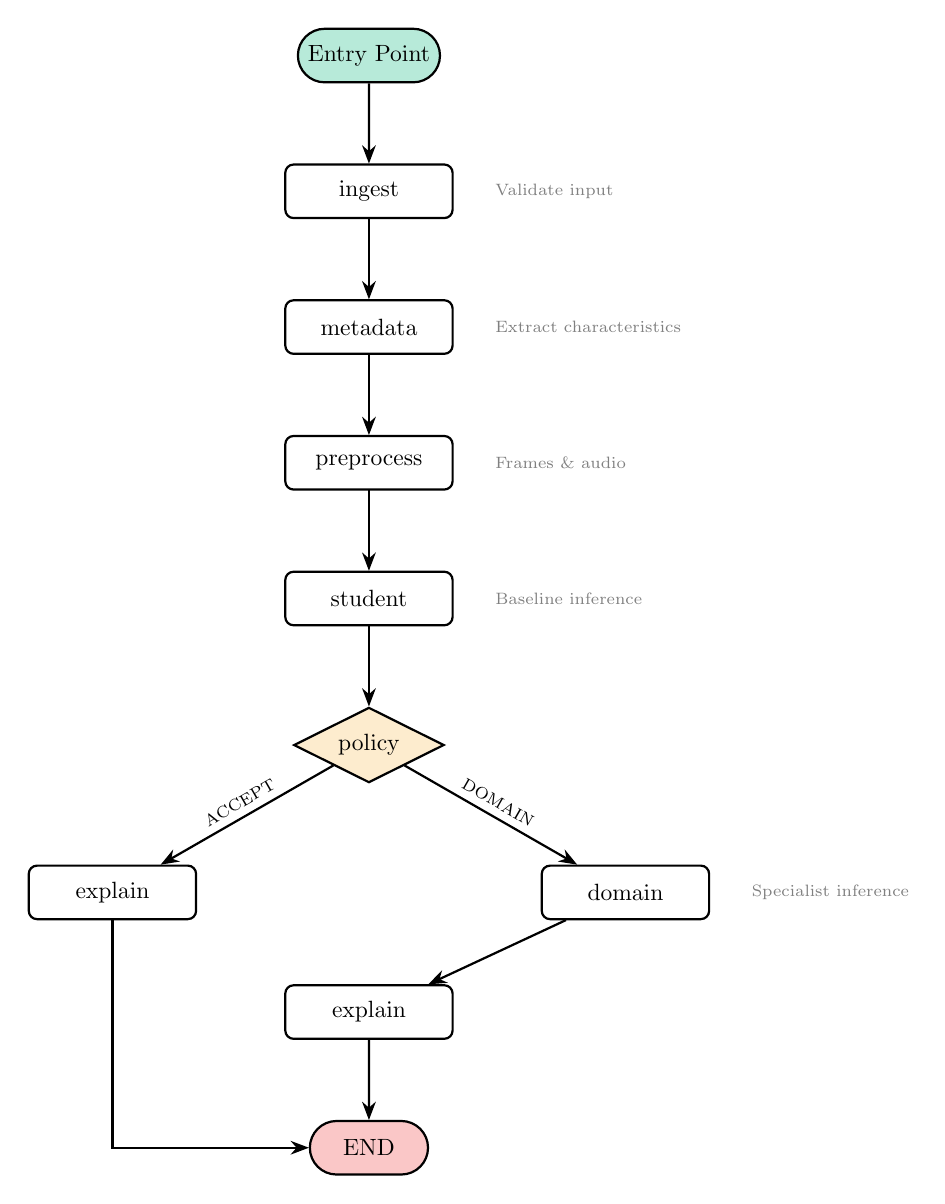
\begin{tikzpicture}[scale=0.85, transform shape, node distance=1.2cm]
    
    % Entry point
    \node[startstop, fill=erakshaAccent!30] (entry) {Entry Point};
    
    % Nodes
    \node[process, below=of entry] (ingest) {ingest};
    \node[process, below=of ingest] (metadata) {metadata};
    \node[process, below=of metadata] (preprocess) {preprocess};
    \node[process, below=of preprocess] (student) {student};
    \node[decision, below=of student] (policy) {policy};
    
    % Conditional branches
    \node[process, below left=1.5cm and 2cm of policy] (explain1) {explain};
    \node[process, below right=1.5cm and 2cm of policy] (domain) {domain};
    
    % Convergence
    \node[process, below=3cm of policy] (explain2) {explain};
    
    % End
    \node[startstop, below=of explain2, fill=erakshaDanger!30] (end) {END};
    
    % Arrows
    \draw[arrow] (entry) -- (ingest);
    \draw[arrow] (ingest) -- (metadata);
    \draw[arrow] (metadata) -- (preprocess);
    \draw[arrow] (preprocess) -- (student);
    \draw[arrow] (student) -- (policy);
    
    \draw[arrow] (policy) -- node[above, sloped, font=\scriptsize] {ACCEPT} (explain1);
    \draw[arrow] (policy) -- node[above, sloped, font=\scriptsize] {DOMAIN} (domain);
    
    \draw[arrow] (explain1) |- (end);
    \draw[arrow] (domain) -- (explain2);
    \draw[arrow] (explain2) -- (end);
    
    % Labels
    \node[right=0.5cm of ingest, font=\scriptsize, text=gray] {Validate input};
    \node[right=0.5cm of metadata, font=\scriptsize, text=gray] {Extract characteristics};
    \node[right=0.5cm of preprocess, font=\scriptsize, text=gray] {Frames \& audio};
    \node[right=0.5cm of student, font=\scriptsize, text=gray] {Baseline inference};
    \node[right=0.5cm of domain, font=\scriptsize, text=gray] {Specialist inference};
    
\end{tikzpicture}
\caption{LangGraph Workflow with Conditional Routing}
\label{fig:langgraph-workflow}
\end{figure}

\subsection{Intelligent Routing Decision Tree}

\begin{figure}[H]
\centering
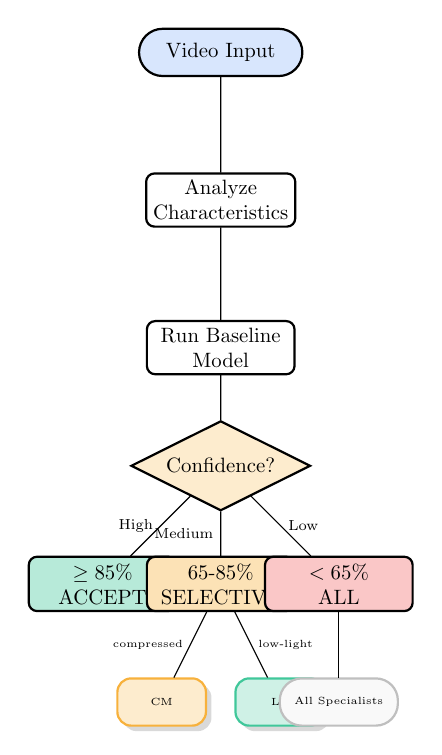
\begin{tikzpicture}[scale=0.75, transform shape,
    level 1/.style={sibling distance=6cm, level distance=2.5cm},
    level 2/.style={sibling distance=3cm, level distance=2.5cm},
    level 3/.style={sibling distance=2cm, level distance=2cm}]
    
    % Root
    \node[startstop, minimum width=3cm] {Video Input}
        child {
            node[process] {Analyze\\Characteristics}
            child {
                node[process] {Run Baseline\\Model}
                child {
                    node[decision, minimum width=2.5cm] {Confidence?}
                    child {
                        node[process, fill=erakshaAccent!30] {$\geq 85\%$\\ACCEPT}
                        edge from parent node[left, font=\scriptsize] {High}
                    }
                    child {
                        node[process, fill=erakshaWarning!30] {65-85\%\\SELECTIVE}
                        child {
                            node[cmmodel, minimum width=1.5cm, minimum height=0.8cm, font=\tiny] {CM}
                            edge from parent node[left, font=\tiny] {compressed}
                        }
                        child {
                            node[llmodel, minimum width=1.5cm, minimum height=0.8cm, font=\tiny] {LL}
                            edge from parent node[right, font=\tiny] {low-light}
                        }
                        edge from parent node[left, font=\scriptsize] {Medium}
                    }
                    child {
                        node[process, fill=erakshaDanger!30] {$< 65\%$\\ALL}
                        child {
                            node[container=gray, minimum width=2cm, minimum height=0.8cm, font=\tiny] {All Specialists}
                        }
                        edge from parent node[right, font=\scriptsize] {Low}
                    }
                }
            }
        };
    
\end{tikzpicture}
\caption{Intelligent Routing Decision Tree}
\label{fig:routing-tree}
\end{figure}

\subsection{Agent Responsibilities Diagram}

\begin{figure}[H]
\centering
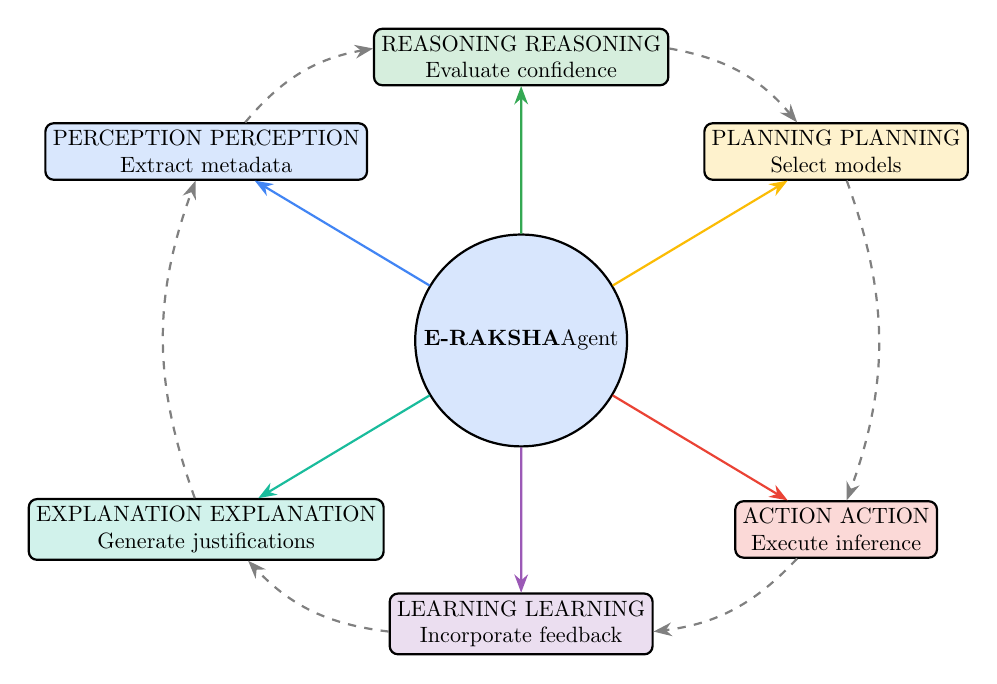
\begin{tikzpicture}[scale=0.8, transform shape]
    
    % Central agent
    \node[draw, circle, minimum size=3cm, fill=erakshaPrimary!20, thick] (agent) at (0,0) {\textbf{E-RAKSHA}\\Agent};
    
    % Responsibilities
    \node[process, fill=convColor!20] (perception) at (-5,3) {PERCEPTION PERCEPTION\\Extract metadata};
    \node[process, fill=bnColor!20] (reasoning) at (0,4.5) {REASONING REASONING\\Evaluate confidence};
    \node[process, fill=reluColor!20] (planning) at (5,3) {PLANNING PLANNING\\Select models};
    \node[process, fill=poolColor!20] (action) at (5,-3) {ACTION ACTION\\Execute inference};
    \node[process, fill=fcColor!20] (learning) at (0,-4.5) {LEARNING LEARNING\\Incorporate feedback};
    \node[process, fill=lstmColor!20] (explanation) at (-5,-3) {EXPLANATION EXPLANATION\\Generate justifications};
    
    % Arrows
    \draw[arrow, convColor] (agent) -- (perception);
    \draw[arrow, bnColor] (agent) -- (reasoning);
    \draw[arrow, reluColor] (agent) -- (planning);
    \draw[arrow, poolColor] (agent) -- (action);
    \draw[arrow, fcColor] (agent) -- (learning);
    \draw[arrow, lstmColor] (agent) -- (explanation);
    
    % Circular flow
    \draw[dashedarrow, gray] (perception) to[bend left=20] (reasoning);
    \draw[dashedarrow, gray] (reasoning) to[bend left=20] (planning);
    \draw[dashedarrow, gray] (planning) to[bend left=20] (action);
    \draw[dashedarrow, gray] (action) to[bend left=20] (learning);
    \draw[dashedarrow, gray] (learning) to[bend left=20] (explanation);
    \draw[dashedarrow, gray] (explanation) to[bend left=20] (perception);
    
\end{tikzpicture}
\caption{Agent Responsibilities and Workflow}
\label{fig:agent-responsibilities}
\end{figure}

\newpage

%%%%%%%%%%%%%%%%%%%%%%%%%%%%%%%%%%%%%%%%%%%%%%%%%%%%%%%%%%%%%%%%%%%%%%%%%%%%%%%
%% SECTION 3: NEURAL NETWORK ARCHITECTURES
%%%%%%%%%%%%%%%%%%%%%%%%%%%%%%%%%%%%%%%%%%%%%%%%%%%%%%%%%%%%%%%%%%%%%%%%%%%%%%%
\section{Neural Network Architectures}

\subsection{Model Bank Overview}

\begin{figure}[H]
\centering
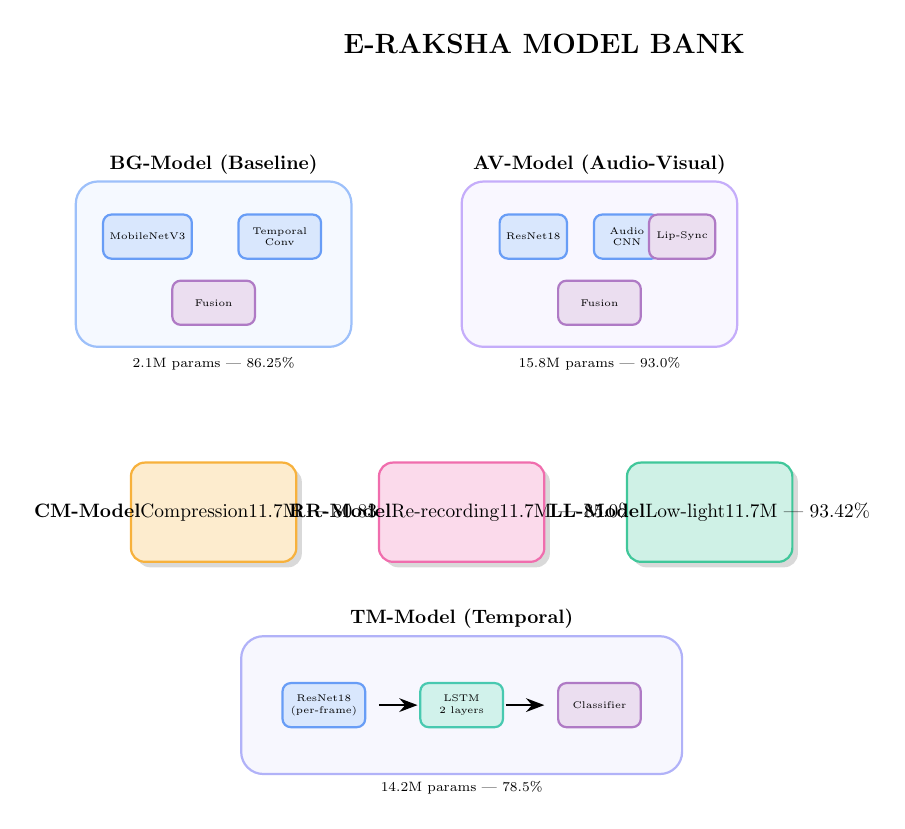
\begin{tikzpicture}[scale=0.7, transform shape]
    
    % Title
    \node[font=\Large\bfseries] at (0,8) {E-RAKSHA MODEL BANK};
    
    % BG-Model (large)
    \begin{scope}[shift={(-6,4)}]
        \node[container=bgModelColor, minimum width=5cm, minimum height=3cm] (bgbox) {};
        \node[above] at (bgbox.north) {\textbf{BG-Model (Baseline)}};
        \node[convlayer, minimum width=1.5cm, font=\tiny] at (-1.2,0.5) {MobileNetV3};
        \node[convlayer, minimum width=1.5cm, font=\tiny] at (1.2,0.5) {Temporal\\Conv};
        \node[fclayer, minimum width=1.5cm, font=\tiny] at (0,-0.7) {Fusion};
        \node[font=\scriptsize] at (0,-1.8) {2.1M params | 86.25\%};
    \end{scope}
    
    % AV-Model (large)
    \begin{scope}[shift={(1,4)}]
        \node[container=avModelColor, minimum width=5cm, minimum height=3cm] (avbox) {};
        \node[above] at (avbox.north) {\textbf{AV-Model (Audio-Visual)}};
        \node[convlayer, minimum width=1.2cm, font=\tiny] at (-1.2,0.5) {ResNet18};
        \node[convlayer, minimum width=1.2cm, font=\tiny] at (0.5,0.5) {Audio\\CNN};
        \node[fclayer, minimum width=1.2cm, font=\tiny] at (1.5,0.5) {Lip-Sync};
        \node[fclayer, minimum width=1.5cm, font=\tiny] at (0,-0.7) {Fusion};
        \node[font=\scriptsize] at (0,-1.8) {15.8M params | 93.0\%};
    \end{scope}
    
    % Specialist Models Row
    \begin{scope}[shift={(-6,-0.5)}]
        \node[cmmodel, minimum width=3cm, minimum height=1.8cm] (cmbox) {};
        \node at (cmbox) {\textbf{CM-Model}\\Compression\\11.7M | 80.83\%};
    \end{scope}
    
    \begin{scope}[shift={(-1.5,-0.5)}]
        \node[rrmodel, minimum width=3cm, minimum height=1.8cm] (rrbox) {};
        \node at (rrbox) {\textbf{RR-Model}\\Re-recording\\11.7M | 85.0\%};
    \end{scope}
    
    \begin{scope}[shift={(3,-0.5)}]
        \node[llmodel, minimum width=3cm, minimum height=1.8cm] (llbox) {};
        \node at (llbox) {\textbf{LL-Model}\\Low-light\\11.7M | 93.42\%};
    \end{scope}
    
    % TM-Model (larger)
    \begin{scope}[shift={(-1.5,-4)}]
        \node[container=tmModelColor, minimum width=8cm, minimum height=2.5cm] (tmbox) {};
        \node[above] at (tmbox.north) {\textbf{TM-Model (Temporal)}};
        \node[convlayer, minimum width=1.5cm, font=\tiny] at (-2.5,0) {ResNet18\\(per-frame)};
        \node[lstmlayer, minimum width=1.5cm, font=\tiny] at (0,0) {LSTM\\2 layers};
        \node[fclayer, minimum width=1.5cm, font=\tiny] at (2.5,0) {Classifier};
        \node[font=\scriptsize] at (0,-1.5) {14.2M params | 78.5\%};
        
        \draw[arrow] (-1.5,0) -- (-0.8,0);
        \draw[arrow] (0.8,0) -- (1.5,0);
    \end{scope}
    
\end{tikzpicture}
\caption{Complete Model Bank Overview with Parameters and Accuracy}
\label{fig:model-bank}
\end{figure}

\subsection{BG-Model (Baseline Generalist) Architecture}

\begin{figure}[H]
\centering
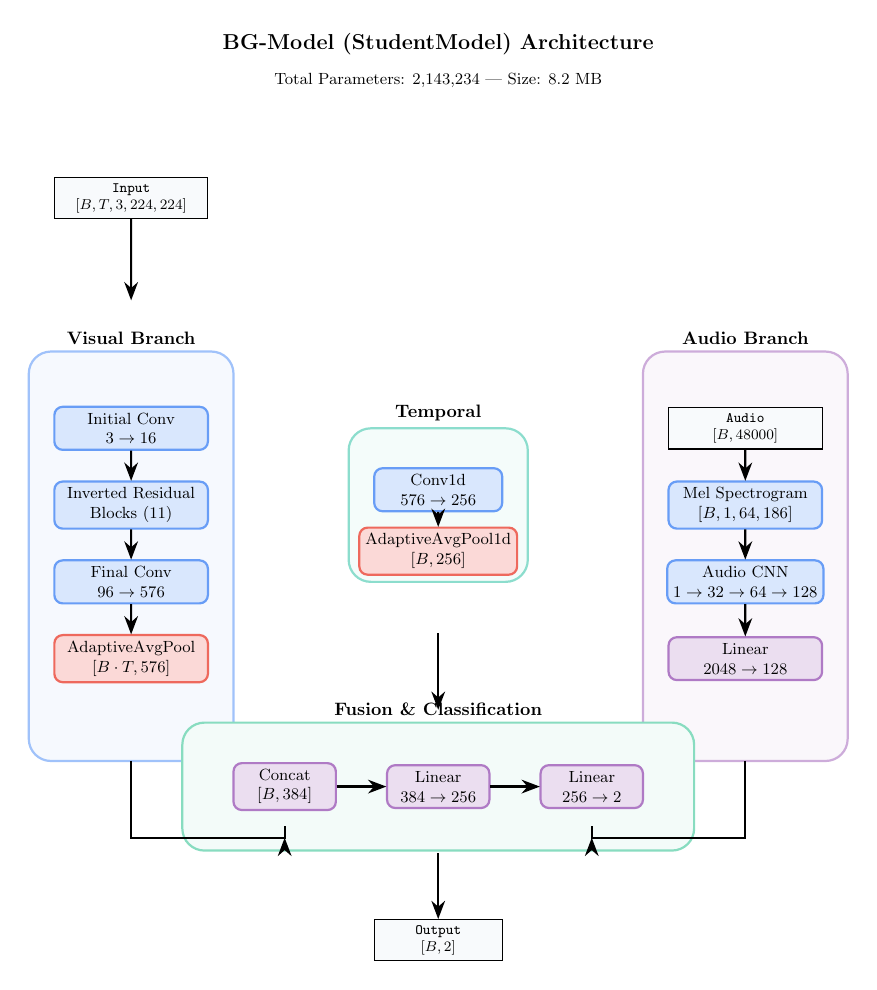
\begin{tikzpicture}[scale=0.65, transform shape, node distance=0.8cm]
    
    % Title
    \node[font=\large\bfseries] at (0,10) {BG-Model (StudentModel) Architecture};
    \node[font=\small] at (0,9.3) {Total Parameters: 2,143,234 | Size: 8.2 MB};
    
    % Input
    \node[tensor, minimum width=3cm] (input) at (-6,7) {Input\\$[B, T, 3, 224, 224]$};
    
    % Visual Branch
    \begin{scope}[shift={(-6,0)}]
        \node[container=convColor, minimum width=4cm, minimum height=8cm] (visualbox) {};
        \node[above, font=\bfseries] at (visualbox.north) {Visual Branch};
        
        % MobileNetV3
        \node[convlayer, minimum width=3cm] (conv1) at (0,2.5) {Initial Conv\\$3 \to 16$};
        \node[convlayer, minimum width=3cm] (invres) at (0,1) {Inverted Residual\\Blocks (11)};
        \node[convlayer, minimum width=3cm] (finalconv) at (0,-0.5) {Final Conv\\$96 \to 576$};
        \node[poollayer, minimum width=3cm] (avgpool) at (0,-2) {AdaptiveAvgPool\\$[B \cdot T, 576]$};
        
        \draw[arrow] (conv1) -- (invres);
        \draw[arrow] (invres) -- (finalconv);
        \draw[arrow] (finalconv) -- (avgpool);
    \end{scope}
    
    % Temporal Processing
    \begin{scope}[shift={(0,1)}]
        \node[container=lstmColor, minimum width=3.5cm, minimum height=3cm] (tempbox) {};
        \node[above, font=\bfseries] at (tempbox.north) {Temporal};
        
        \node[convlayer, minimum width=2.5cm] (tempconv) at (0,0.3) {Conv1d\\$576 \to 256$};
        \node[poollayer, minimum width=2.5cm] (temppool) at (0,-0.9) {AdaptiveAvgPool1d\\$[B, 256]$};
        
        \draw[arrow] (tempconv) -- (temppool);
    \end{scope}
    
    % Audio Branch
    \begin{scope}[shift={(6,0)}]
        \node[container=fcColor, minimum width=4cm, minimum height=8cm] (audiobox) {};
        \node[above, font=\bfseries] at (audiobox.north) {Audio Branch};
        
        \node[tensor, minimum width=3cm] (audioin) at (0,2.5) {Audio\\$[B, 48000]$};
        \node[convlayer, minimum width=3cm] (mel) at (0,1) {Mel Spectrogram\\$[B, 1, 64, 186]$};
        \node[convlayer, minimum width=3cm] (audiocnn) at (0,-0.5) {Audio CNN\\$1 \to 32 \to 64 \to 128$};
        \node[fclayer, minimum width=3cm] (audiofc) at (0,-2) {Linear\\$2048 \to 128$};
        
        \draw[arrow] (audioin) -- (mel);
        \draw[arrow] (mel) -- (audiocnn);
        \draw[arrow] (audiocnn) -- (audiofc);
    \end{scope}
    
    % Fusion
    \begin{scope}[shift={(0,-4.5)}]
        \node[container=erakshaAccent, minimum width=10cm, minimum height=2.5cm] (fusionbox) {};
        \node[above, font=\bfseries] at (fusionbox.north) {Fusion \& Classification};
        
        \node[fclayer, minimum width=2cm] (concat) at (-3,0) {Concat\\$[B, 384]$};
        \node[fclayer, minimum width=2cm] (fc1) at (0,0) {Linear\\$384 \to 256$};
        \node[fclayer, minimum width=2cm] (fc2) at (3,0) {Linear\\$256 \to 2$};
        
        \draw[arrow] (concat) -- (fc1);
        \draw[arrow] (fc1) -- (fc2);
    \end{scope}
    
    % Output
    \node[tensor, minimum width=2.5cm] (output) at (0,-7.5) {Output\\$[B, 2]$};
    
    % Connections
    \draw[arrow] (input) -- (-6,5);
    \draw[arrow] (-6,-4) -- (-6,-5.5) -| (-3,-5.5);
    \draw[arrow] (0,-1.5) -- (0,-3);
    \draw[arrow] (6,-4) -- (6,-5.5) -| (3,-5.5);
    \draw[arrow] (0,-5.8) -- (output);
    
\end{tikzpicture}
\caption{BG-Model (StudentModel) Complete Architecture}
\label{fig:bg-model}
\end{figure}

\subsection{MobileNetV3-Small Backbone Detail}

\begin{figure}[H]
\centering
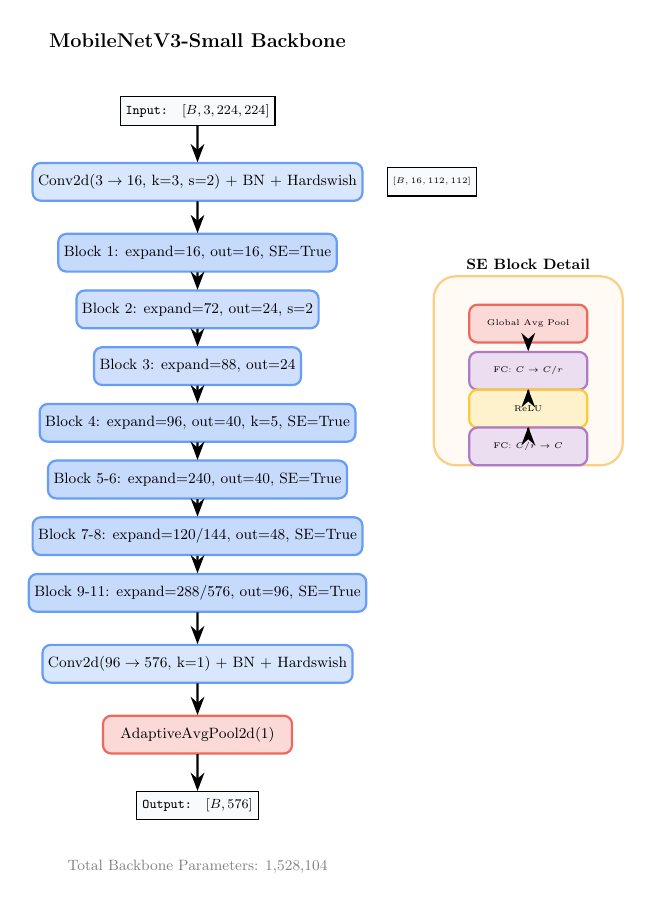
\begin{tikzpicture}[scale=0.6, transform shape, node distance=0.5cm]
    
    % Title
    \node[font=\large\bfseries] at (0,12) {MobileNetV3-Small Backbone};
    
    % Input
    \node[tensor] (input) at (0,10.5) {Input: $[B, 3, 224, 224]$};
    
    % Initial Conv
    \node[convlayer, minimum width=4cm] (conv1) at (0,9) {Conv2d($3 \to 16$, k=3, s=2) + BN + Hardswish};
    \node[tensor, right=0.5cm of conv1, font=\tiny] {$[B, 16, 112, 112]$};
    
    % Inverted Residual Blocks
    \node[convlayer, minimum width=4cm, fill=convColor!30] (block1) at (0,7.5) {Block 1: expand=16, out=16, SE=True};
    \node[convlayer, minimum width=4cm, fill=convColor!25] (block2) at (0,6.3) {Block 2: expand=72, out=24, s=2};
    \node[convlayer, minimum width=4cm, fill=convColor!25] (block3) at (0,5.1) {Block 3: expand=88, out=24};
    \node[convlayer, minimum width=4cm, fill=convColor!30] (block4) at (0,3.9) {Block 4: expand=96, out=40, k=5, SE=True};
    \node[convlayer, minimum width=4cm, fill=convColor!30] (block5) at (0,2.7) {Block 5-6: expand=240, out=40, SE=True};
    \node[convlayer, minimum width=4cm, fill=convColor!30] (block7) at (0,1.5) {Block 7-8: expand=120/144, out=48, SE=True};
    \node[convlayer, minimum width=4cm, fill=convColor!30] (block9) at (0,0.3) {Block 9-11: expand=288/576, out=96, SE=True};
    
    % Final Conv
    \node[convlayer, minimum width=4cm] (finalconv) at (0,-1.2) {Conv2d($96 \to 576$, k=1) + BN + Hardswish};
    
    % Pooling
    \node[poollayer, minimum width=4cm] (pool) at (0,-2.7) {AdaptiveAvgPool2d(1)};
    
    % Output
    \node[tensor] (output) at (0,-4.2) {Output: $[B, 576]$};
    
    % Arrows
    \draw[arrow] (input) -- (conv1);
    \draw[arrow] (conv1) -- (block1);
    \draw[arrow] (block1) -- (block2);
    \draw[arrow] (block2) -- (block3);
    \draw[arrow] (block3) -- (block4);
    \draw[arrow] (block4) -- (block5);
    \draw[arrow] (block5) -- (block7);
    \draw[arrow] (block7) -- (block9);
    \draw[arrow] (block9) -- (finalconv);
    \draw[arrow] (finalconv) -- (pool);
    \draw[arrow] (pool) -- (output);
    
    % SE Block detail
    \begin{scope}[shift={(7,5)}]
        \node[container=erakshaWarning, minimum width=4cm, minimum height=4cm] (sebox) {};
        \node[above, font=\bfseries\small] at (sebox.north) {SE Block Detail};
        
        \node[poollayer, minimum width=2.5cm, font=\tiny] (segap) at (0,1) {Global Avg Pool};
        \node[fclayer, minimum width=2.5cm, font=\tiny] (sefc1) at (0,0) {FC: $C \to C/r$};
        \node[relulayer, minimum width=2.5cm, font=\tiny] (serelu) at (0,-0.8) {ReLU};
        \node[fclayer, minimum width=2.5cm, font=\tiny] (sefc2) at (0,-1.6) {FC: $C/r \to C$};
        
        \draw[arrow, font=\tiny] (segap) -- (sefc1);
        \draw[arrow] (sefc1) -- (serelu);
        \draw[arrow] (serelu) -- (sefc2);
    \end{scope}
    
    % Parameters
    \node[font=\small, text=gray] at (0,-5.5) {Total Backbone Parameters: 1,528,104};
    
\end{tikzpicture}
\caption{MobileNetV3-Small Backbone Architecture with SE Blocks}
\label{fig:mobilenetv3}
\end{figure}

\subsection{AV-Model (Audio-Visual Specialist) Architecture}

\begin{figure}[H]
\centering
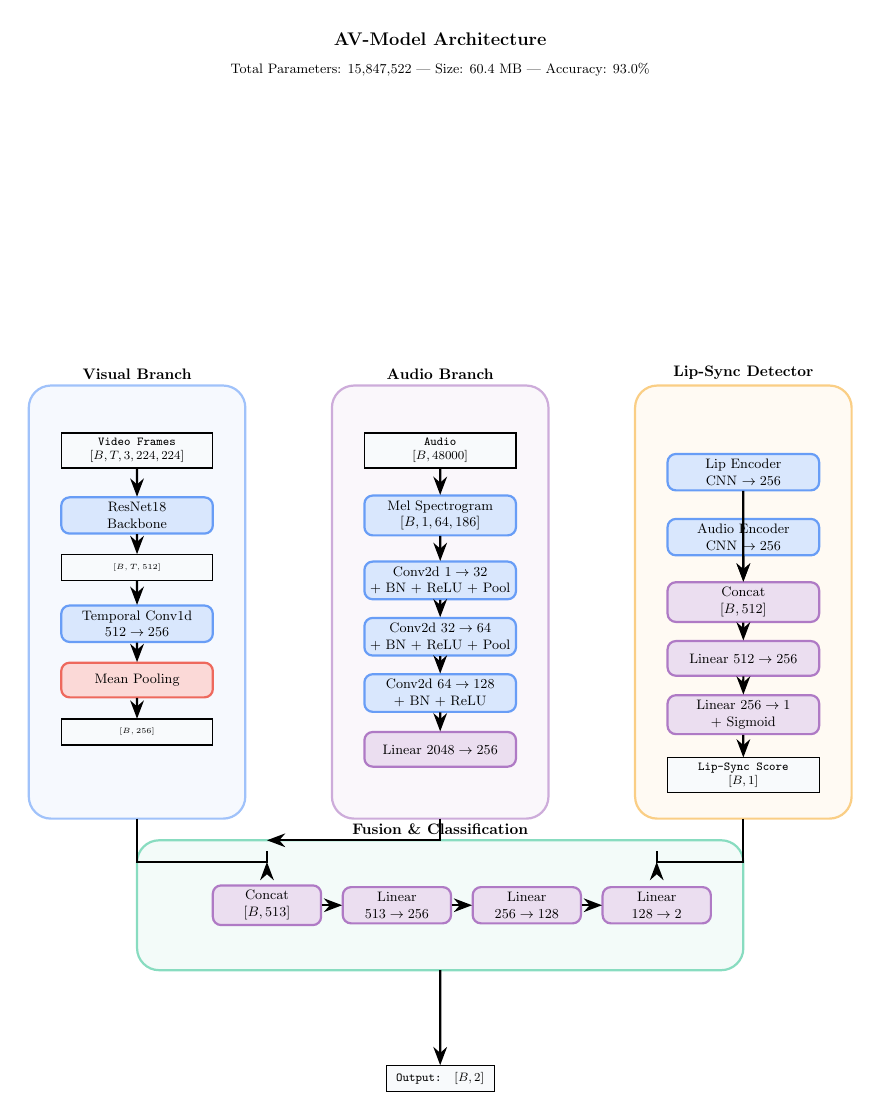
\begin{tikzpicture}[scale=0.55, transform shape, node distance=0.6cm]
    
    % Title
    \node[font=\large\bfseries] at (0,13) {AV-Model Architecture};
    \node[font=\small] at (0,12.3) {Total Parameters: 15,847,522 | Size: 60.4 MB | Accuracy: 93.0\%};
    
    % Visual Branch
    \begin{scope}[shift={(-7,0)}]
        \node[container=convColor, minimum width=5cm, minimum height=10cm] (visualbox) {};
        \node[above, font=\bfseries] at (visualbox.north) {Visual Branch};
        
        \node[tensor, minimum width=3.5cm] (vidin) at (0,3.5) {Video Frames\\$[B, T, 3, 224, 224]$};
        
        \node[convlayer, minimum width=3.5cm] (resnet) at (0,2) {ResNet18\\Backbone};
        \node[tensor, minimum width=3.5cm, font=\tiny] (resfeat) at (0,0.8) {$[B, T, 512]$};
        
        \node[convlayer, minimum width=3.5cm] (tempconv) at (0,-0.5) {Temporal Conv1d\\$512 \to 256$};
        \node[poollayer, minimum width=3.5cm] (temppool) at (0,-1.8) {Mean Pooling};
        \node[tensor, minimum width=3.5cm, font=\tiny] (vidfeat) at (0,-3) {$[B, 256]$};
        
        \draw[arrow] (vidin) -- (resnet);
        \draw[arrow] (resnet) -- (resfeat);
        \draw[arrow] (resfeat) -- (tempconv);
        \draw[arrow] (tempconv) -- (temppool);
        \draw[arrow] (temppool) -- (vidfeat);
    \end{scope}
    
    % Audio Branch
    \begin{scope}[shift={(0,0)}]
        \node[container=fcColor, minimum width=5cm, minimum height=10cm] (audiobox) {};
        \node[above, font=\bfseries] at (audiobox.north) {Audio Branch};
        
        \node[tensor, minimum width=3.5cm] (audin) at (0,3.5) {Audio\\$[B, 48000]$};
        
        \node[convlayer, minimum width=3.5cm] (mel) at (0,2) {Mel Spectrogram\\$[B, 1, 64, 186]$};
        
        \node[convlayer, minimum width=3.5cm] (audcnn1) at (0,0.5) {Conv2d $1 \to 32$\\+ BN + ReLU + Pool};
        \node[convlayer, minimum width=3.5cm] (audcnn2) at (0,-0.8) {Conv2d $32 \to 64$\\+ BN + ReLU + Pool};
        \node[convlayer, minimum width=3.5cm] (audcnn3) at (0,-2.1) {Conv2d $64 \to 128$\\+ BN + ReLU};
        \node[fclayer, minimum width=3.5cm] (audfc) at (0,-3.4) {Linear $2048 \to 256$};
        
        \draw[arrow] (audin) -- (mel);
        \draw[arrow] (mel) -- (audcnn1);
        \draw[arrow] (audcnn1) -- (audcnn2);
        \draw[arrow] (audcnn2) -- (audcnn3);
        \draw[arrow] (audcnn3) -- (audfc);
    \end{scope}
    
    % Lip-Sync Detector
    \begin{scope}[shift={(7,0)}]
        \node[container=erakshaWarning, minimum width=5cm, minimum height=10cm] (lipsyncbox) {};
        \node[above, font=\bfseries] at (lipsyncbox.north) {Lip-Sync Detector};
        
        \node[convlayer, minimum width=3.5cm] (lipenc) at (0,3) {Lip Encoder\\CNN $\to 256$};
        \node[convlayer, minimum width=3.5cm] (audenc) at (0,1.5) {Audio Encoder\\CNN $\to 256$};
        
        \node[fclayer, minimum width=3.5cm] (concat) at (0,0) {Concat\\$[B, 512]$};
        \node[fclayer, minimum width=3.5cm] (syncfc1) at (0,-1.3) {Linear $512 \to 256$};
        \node[fclayer, minimum width=3.5cm] (syncfc2) at (0,-2.6) {Linear $256 \to 1$\\+ Sigmoid};
        \node[tensor, minimum width=3.5cm] (syncscore) at (0,-4) {Lip-Sync Score\\$[B, 1]$};
        
        \draw[arrow] (lipenc) -- (concat);
        \draw[arrow] (audenc) -- (concat);
        \draw[arrow] (concat) -- (syncfc1);
        \draw[arrow] (syncfc1) -- (syncfc2);
        \draw[arrow] (syncfc2) -- (syncscore);
    \end{scope}
    
    % Fusion
    \begin{scope}[shift={(0,-7)}]
        \node[container=erakshaAccent, minimum width=14cm, minimum height=3cm] (fusionbox) {};
        \node[above, font=\bfseries] at (fusionbox.north) {Fusion \& Classification};
        
        \node[fclayer, minimum width=2.5cm] (fconcat) at (-4,0) {Concat\\$[B, 513]$};
        \node[fclayer, minimum width=2.5cm] (ffc1) at (-1,0) {Linear\\$513 \to 256$};
        \node[fclayer, minimum width=2.5cm] (ffc2) at (2,0) {Linear\\$256 \to 128$};
        \node[fclayer, minimum width=2.5cm] (ffc3) at (5,0) {Linear\\$128 \to 2$};
        
        \draw[arrow] (fconcat) -- (ffc1);
        \draw[arrow] (ffc1) -- (ffc2);
        \draw[arrow] (ffc2) -- (ffc3);
    \end{scope}
    
    % Output
    \node[tensor, minimum width=2.5cm] (output) at (0,-11) {Output: $[B, 2]$};
    
    % Connections to fusion
    \draw[arrow] (-7,-5) -- (-7,-6) -| (-4,-6);
    \draw[arrow] (0,-5) -- (0,-5.5) -- (-4,-5.5);
    \draw[arrow] (7,-5) -- (7,-6) -| (5,-6);
    \draw[arrow] (0,-8.5) -- (output);
    
\end{tikzpicture}
\caption{AV-Model Complete Architecture with Lip-Sync Detection}
\label{fig:av-model}
\end{figure}

\newpage

\subsection{ResNet18 Backbone Architecture}

\begin{figure}[H]
\centering
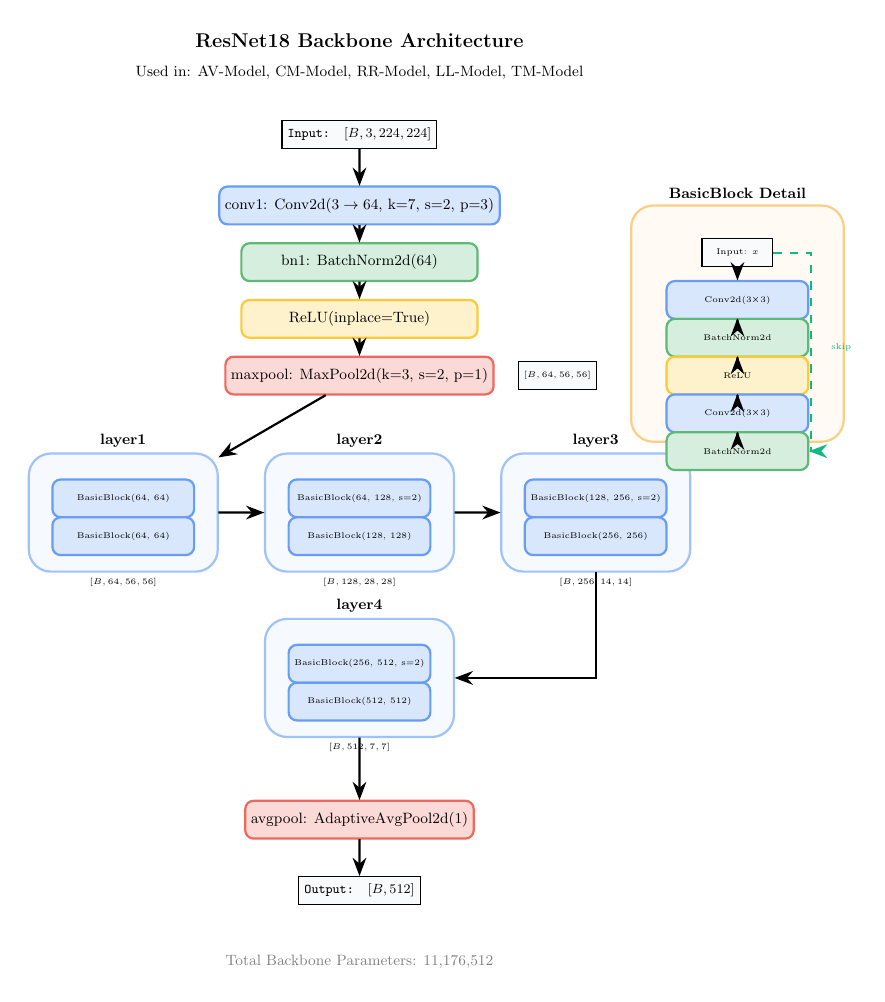
\begin{tikzpicture}[scale=0.6, transform shape, node distance=0.5cm]
    
    % Title
    \node[font=\large\bfseries] at (0,14) {ResNet18 Backbone Architecture};
    \node[font=\small] at (0,13.3) {Used in: AV-Model, CM-Model, RR-Model, LL-Model, TM-Model};
    
    % Input
    \node[tensor] (input) at (0,12) {Input: $[B, 3, 224, 224]$};
    
    % Initial layers
    \node[convlayer, minimum width=5cm] (conv1) at (0,10.5) {conv1: Conv2d($3 \to 64$, k=7, s=2, p=3)};
    \node[bnlayer, minimum width=5cm] (bn1) at (0,9.3) {bn1: BatchNorm2d(64)};
    \node[relulayer, minimum width=5cm] (relu) at (0,8.1) {ReLU(inplace=True)};
    \node[poollayer, minimum width=5cm] (maxpool) at (0,6.9) {maxpool: MaxPool2d(k=3, s=2, p=1)};
    
    \node[tensor, right=0.5cm of maxpool, font=\tiny] {$[B, 64, 56, 56]$};
    
    % Layer 1
    \begin{scope}[shift={(-5,4)}]
        \node[container=convColor, minimum width=4cm, minimum height=2.5cm] (layer1) {};
        \node[above, font=\bfseries\small] at (layer1.north) {layer1};
        \node[convlayer, minimum width=3cm, font=\tiny] at (0,0.3) {BasicBlock(64, 64)};
        \node[convlayer, minimum width=3cm, font=\tiny] at (0,-0.5) {BasicBlock(64, 64)};
        \node[below, font=\tiny] at (layer1.south) {$[B, 64, 56, 56]$};
    \end{scope}
    
    % Layer 2
    \begin{scope}[shift={(0,4)}]
        \node[container=convColor, minimum width=4cm, minimum height=2.5cm] (layer2) {};
        \node[above, font=\bfseries\small] at (layer2.north) {layer2};
        \node[convlayer, minimum width=3cm, font=\tiny] at (0,0.3) {BasicBlock(64, 128, s=2)};
        \node[convlayer, minimum width=3cm, font=\tiny] at (0,-0.5) {BasicBlock(128, 128)};
        \node[below, font=\tiny] at (layer2.south) {$[B, 128, 28, 28]$};
    \end{scope}
    
    % Layer 3
    \begin{scope}[shift={(5,4)}]
        \node[container=convColor, minimum width=4cm, minimum height=2.5cm] (layer3) {};
        \node[above, font=\bfseries\small] at (layer3.north) {layer3};
        \node[convlayer, minimum width=3cm, font=\tiny] at (0,0.3) {BasicBlock(128, 256, s=2)};
        \node[convlayer, minimum width=3cm, font=\tiny] at (0,-0.5) {BasicBlock(256, 256)};
        \node[below, font=\tiny] at (layer3.south) {$[B, 256, 14, 14]$};
    \end{scope}
    
    % Layer 4
    \begin{scope}[shift={(0,0.5)}]
        \node[container=convColor, minimum width=4cm, minimum height=2.5cm] (layer4) {};
        \node[above, font=\bfseries\small] at (layer4.north) {layer4};
        \node[convlayer, minimum width=3cm, font=\tiny] at (0,0.3) {BasicBlock(256, 512, s=2)};
        \node[convlayer, minimum width=3cm, font=\tiny] at (0,-0.5) {BasicBlock(512, 512)};
        \node[below, font=\tiny] at (layer4.south) {$[B, 512, 7, 7]$};
    \end{scope}
    
    % Average Pool
    \node[poollayer, minimum width=4cm] (avgpool) at (0,-2.5) {avgpool: AdaptiveAvgPool2d(1)};
    
    % Output
    \node[tensor] (output) at (0,-4) {Output: $[B, 512]$};
    
    % Arrows
    \draw[arrow] (input) -- (conv1);
    \draw[arrow] (conv1) -- (bn1);
    \draw[arrow] (bn1) -- (relu);
    \draw[arrow] (relu) -- (maxpool);
    \draw[arrow] (maxpool) -- (layer1);
    \draw[arrow] (layer1) -- (layer2);
    \draw[arrow] (layer2) -- (layer3);
    \draw[arrow] (layer3) |- (layer4);
    \draw[arrow] (layer4) -- (avgpool);
    \draw[arrow] (avgpool) -- (output);
    
    % BasicBlock detail
    \begin{scope}[shift={(8,8)}]
        \node[container=erakshaWarning, minimum width=4.5cm, minimum height=5cm] (bbbox) {};
        \node[above, font=\bfseries\small] at (bbbox.north) {BasicBlock Detail};
        
        \node[tensor, font=\tiny] (bbin) at (0,1.5) {Input: $x$};
        \node[convlayer, minimum width=3cm, font=\tiny] (bbconv1) at (0,0.5) {Conv2d(3×3)};
        \node[bnlayer, minimum width=3cm, font=\tiny] (bbbn1) at (0,-0.3) {BatchNorm2d};
        \node[relulayer, minimum width=3cm, font=\tiny] (bbrelu1) at (0,-1.1) {ReLU};
        \node[convlayer, minimum width=3cm, font=\tiny] (bbconv2) at (0,-1.9) {Conv2d(3×3)};
        \node[bnlayer, minimum width=3cm, font=\tiny] (bbbn2) at (0,-2.7) {BatchNorm2d};
        
        \draw[arrow] (bbin) -- (bbconv1);
        \draw[arrow] (bbconv1) -- (bbbn1);
        \draw[arrow] (bbbn1) -- (bbrelu1);
        \draw[arrow] (bbrelu1) -- (bbconv2);
        \draw[arrow] (bbconv2) -- (bbbn2);
        
        % Skip connection
        \draw[arrow, dashed, erakshaAccent] (bbin.east) -- ++(0.8,0) |- (bbbn2.east);
        \node[font=\tiny, text=erakshaAccent] at (2.2,-0.5) {skip};
    \end{scope}
    
    % Parameters
    \node[font=\small, text=gray] at (0,-5.5) {Total Backbone Parameters: 11,176,512};
    
\end{tikzpicture}
\caption{ResNet18 Backbone with BasicBlock Detail}
\label{fig:resnet18}
\end{figure}

\subsection{Specialist Model Architecture (CM, RR, LL)}

\begin{figure}[H]
\centering
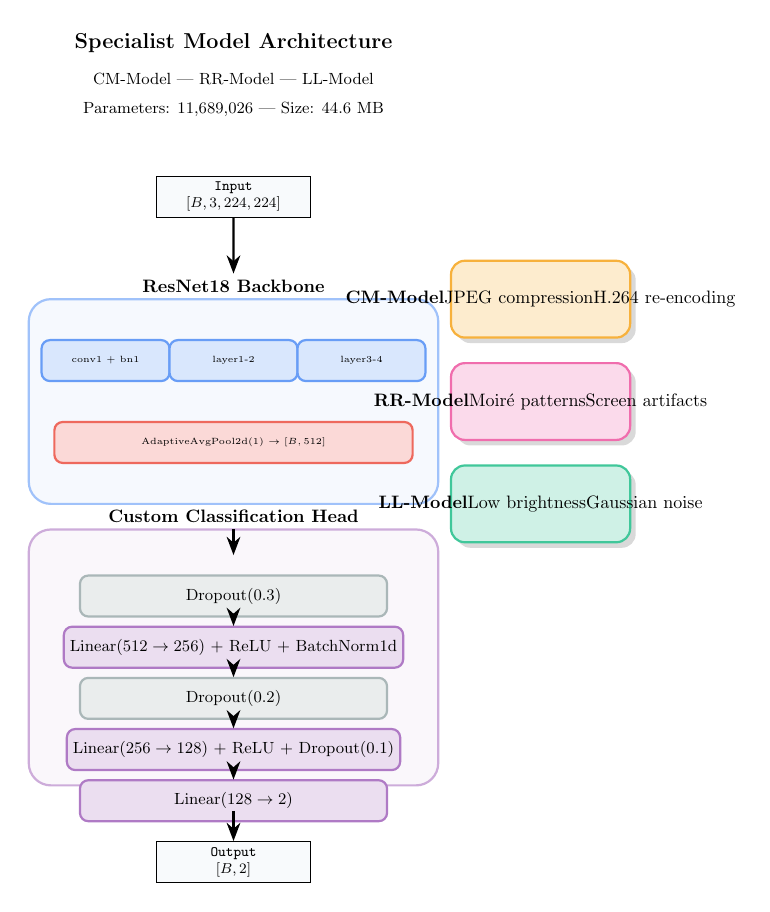
\begin{tikzpicture}[scale=0.65, transform shape, node distance=0.6cm]
    
    % Title
    \node[font=\large\bfseries] at (0,10) {Specialist Model Architecture};
    \node[font=\small] at (0,9.3) {CM-Model | RR-Model | LL-Model};
    \node[font=\small] at (0,8.7) {Parameters: 11,689,026 | Size: 44.6 MB};
    
    % Input
    \node[tensor, minimum width=3cm] (input) at (0,7) {Input\\$[B, 3, 224, 224]$};
    
    % ResNet18 Backbone
    \begin{scope}[shift={(0,3)}]
        \node[container=convColor, minimum width=8cm, minimum height=4cm] (backbone) {};
        \node[above, font=\bfseries] at (backbone.north) {ResNet18 Backbone};
        
        \node[convlayer, minimum width=2.5cm, font=\tiny] at (-2.5,0.8) {conv1 + bn1};
        \node[convlayer, minimum width=2.5cm, font=\tiny] at (0,0.8) {layer1-2};
        \node[convlayer, minimum width=2.5cm, font=\tiny] at (2.5,0.8) {layer3-4};
        \node[poollayer, minimum width=7cm, font=\tiny] at (0,-0.8) {AdaptiveAvgPool2d(1) $\to [B, 512]$};
    \end{scope}
    
    % Classification Head
    \begin{scope}[shift={(0,-2)}]
        \node[container=fcColor, minimum width=8cm, minimum height=5cm] (head) {};
        \node[above, font=\bfseries] at (head.north) {Custom Classification Head};
        
        \node[dropoutlayer, minimum width=6cm] (drop1) at (0,1.2) {Dropout(0.3)};
        \node[fclayer, minimum width=6cm] (fc1) at (0,0.2) {Linear($512 \to 256$) + ReLU + BatchNorm1d};
        \node[dropoutlayer, minimum width=6cm] (drop2) at (0,-0.8) {Dropout(0.2)};
        \node[fclayer, minimum width=6cm] (fc2) at (0,-1.8) {Linear($256 \to 128$) + ReLU + Dropout(0.1)};
        \node[fclayer, minimum width=6cm] (fc3) at (0,-2.8) {Linear($128 \to 2$)};
        
        \draw[arrow] (drop1) -- (fc1);
        \draw[arrow] (fc1) -- (drop2);
        \draw[arrow] (drop2) -- (fc2);
        \draw[arrow] (fc2) -- (fc3);
    \end{scope}
    
    % Output
    \node[tensor, minimum width=3cm] (output) at (0,-6) {Output\\$[B, 2]$};
    
    % Arrows
    \draw[arrow] (input) -- (0,5.5);
    \draw[arrow] (0,0.5) -- (0,0);
    \draw[arrow] (0,-5) -- (output);
    
    % Training specialization boxes
    \begin{scope}[shift={(6,3)}]
        \node[cmmodel, minimum width=3.5cm, minimum height=1.5cm] (cmspec) at (0,2) {};
        \node at (cmspec) {\textbf{CM-Model}\\JPEG compression\\H.264 re-encoding};
        
        \node[rrmodel, minimum width=3.5cm, minimum height=1.5cm] (rrspec) at (0,0) {};
        \node at (rrspec) {\textbf{RR-Model}\\Moiré patterns\\Screen artifacts};
        
        \node[llmodel, minimum width=3.5cm, minimum height=1.5cm] (llspec) at (0,-2) {};
        \node at (llspec) {\textbf{LL-Model}\\Low brightness\\Gaussian noise};
    \end{scope}
    
\end{tikzpicture}
\caption{Specialist Model Architecture with Training Specializations}
\label{fig:specialist-model}
\end{figure}

\subsection{TM-Model (Temporal Specialist) Architecture}

\begin{figure}[H]
\centering
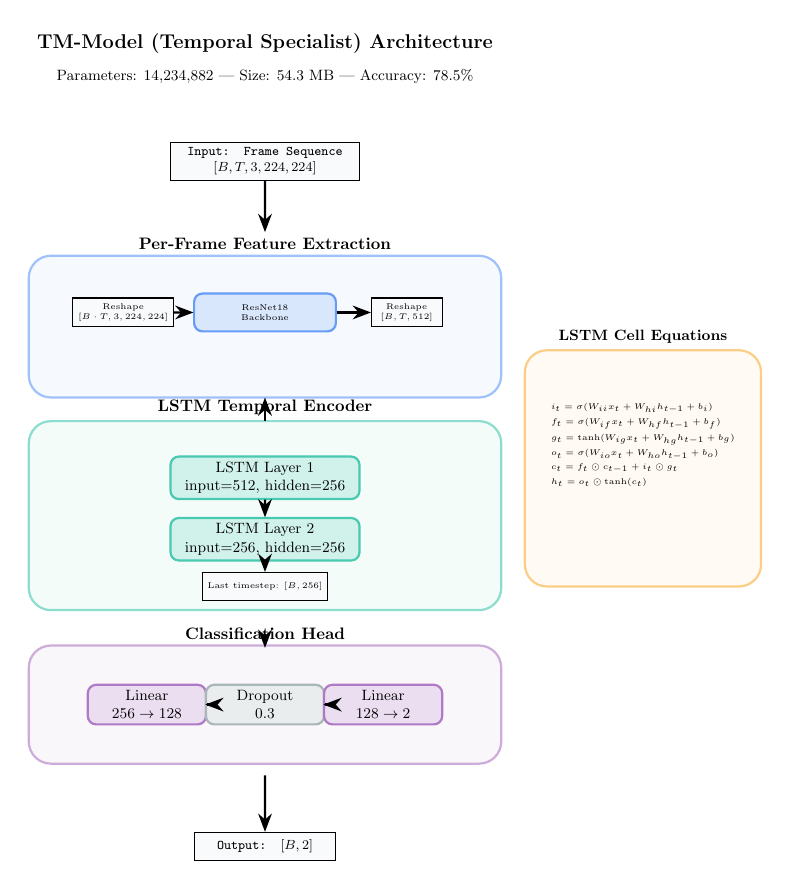
\begin{tikzpicture}[scale=0.6, transform shape, node distance=0.6cm]
    
    % Title
    \node[font=\large\bfseries] at (0,11) {TM-Model (Temporal Specialist) Architecture};
    \node[font=\small] at (0,10.3) {Parameters: 14,234,882 | Size: 54.3 MB | Accuracy: 78.5\%};
    
    % Input
    \node[tensor, minimum width=4cm] (input) at (0,8.5) {Input: Frame Sequence\\$[B, T, 3, 224, 224]$};
    
    % Per-frame processing
    \begin{scope}[shift={(0,5)}]
        \node[container=convColor, minimum width=10cm, minimum height=3cm] (perframe) {};
        \node[above, font=\bfseries] at (perframe.north) {Per-Frame Feature Extraction};
        
        \node[tensor, font=\tiny] (reshape1) at (-3,0.3) {Reshape\\$[B \cdot T, 3, 224, 224]$};
        \node[convlayer, minimum width=3cm, font=\tiny] (resnet) at (0,0.3) {ResNet18\\Backbone};
        \node[tensor, font=\tiny] (reshape2) at (3,0.3) {Reshape\\$[B, T, 512]$};
        
        \draw[arrow] (reshape1) -- (resnet);
        \draw[arrow] (resnet) -- (reshape2);
    \end{scope}
    
    % LSTM Processing
    \begin{scope}[shift={(0,1)}]
        \node[container=lstmColor, minimum width=10cm, minimum height=4cm] (lstmbox) {};
        \node[above, font=\bfseries] at (lstmbox.north) {LSTM Temporal Encoder};
        
        \node[lstmlayer, minimum width=4cm] (lstm1) at (0,0.8) {LSTM Layer 1\\input=512, hidden=256};
        \node[lstmlayer, minimum width=4cm] (lstm2) at (0,-0.5) {LSTM Layer 2\\input=256, hidden=256};
        \node[tensor, font=\tiny] (lstmout) at (0,-1.5) {Last timestep: $[B, 256]$};
        
        \draw[arrow] (lstm1) -- (lstm2);
        \draw[arrow] (lstm2) -- (lstmout);
    \end{scope}
    
    % Classification Head
    \begin{scope}[shift={(0,-3)}]
        \node[container=fcColor, minimum width=10cm, minimum height=2.5cm] (classhead) {};
        \node[above, font=\bfseries] at (classhead.north) {Classification Head};
        
        \node[fclayer, minimum width=2.5cm] (fc1) at (-2.5,0) {Linear\\$256 \to 128$};
        \node[dropoutlayer, minimum width=2.5cm] (drop) at (0,0) {Dropout\\0.3};
        \node[fclayer, minimum width=2.5cm] (fc2) at (2.5,0) {Linear\\$128 \to 2$};
        
        \draw[arrow] (fc1) -- (drop);
        \draw[arrow] (drop) -- (fc2);
    \end{scope}
    
    % Output
    \node[tensor, minimum width=3cm] (output) at (0,-6) {Output: $[B, 2]$};
    
    % Arrows
    \draw[arrow] (input) -- (0,7);
    \draw[arrow] (0,3) -- (0,3.5);
    \draw[arrow] (0,-1.5) -- (0,-1.8);
    \draw[arrow] (0,-4.5) -- (output);
    
    % LSTM Cell detail
    \begin{scope}[shift={(8,2)}]
        \node[container=erakshaWarning, minimum width=5cm, minimum height=5cm] (lstmcell) {};
        \node[above, font=\bfseries\small] at (lstmcell.north) {LSTM Cell Equations};
        
        \node[font=\tiny, align=left] at (0,0.5) {
            $i_t = \sigma(W_{ii}x_t + W_{hi}h_{t-1} + b_i)$\\[2pt]
            $f_t = \sigma(W_{if}x_t + W_{hf}h_{t-1} + b_f)$\\[2pt]
            $g_t = \tanh(W_{ig}x_t + W_{hg}h_{t-1} + b_g)$\\[2pt]
            $o_t = \sigma(W_{io}x_t + W_{ho}h_{t-1} + b_o)$\\[2pt]
            $c_t = f_t \odot c_{t-1} + i_t \odot g_t$\\[2pt]
            $h_t = o_t \odot \tanh(c_t)$
        };
    \end{scope}
    
\end{tikzpicture}
\caption{TM-Model Architecture with LSTM Temporal Encoder}
\label{fig:tm-model}
\end{figure}

\newpage

%%%%%%%%%%%%%%%%%%%%%%%%%%%%%%%%%%%%%%%%%%%%%%%%%%%%%%%%%%%%%%%%%%%%%%%%%%%%%%%
%% SECTION 4: ENSEMBLE AND AGGREGATION
%%%%%%%%%%%%%%%%%%%%%%%%%%%%%%%%%%%%%%%%%%%%%%%%%%%%%%%%%%%%%%%%%%%%%%%%%%%%%%%
\section{Ensemble Architecture and Aggregation}

\subsection{Dynamic Ensemble Architecture}

\begin{figure}[H]
\centering
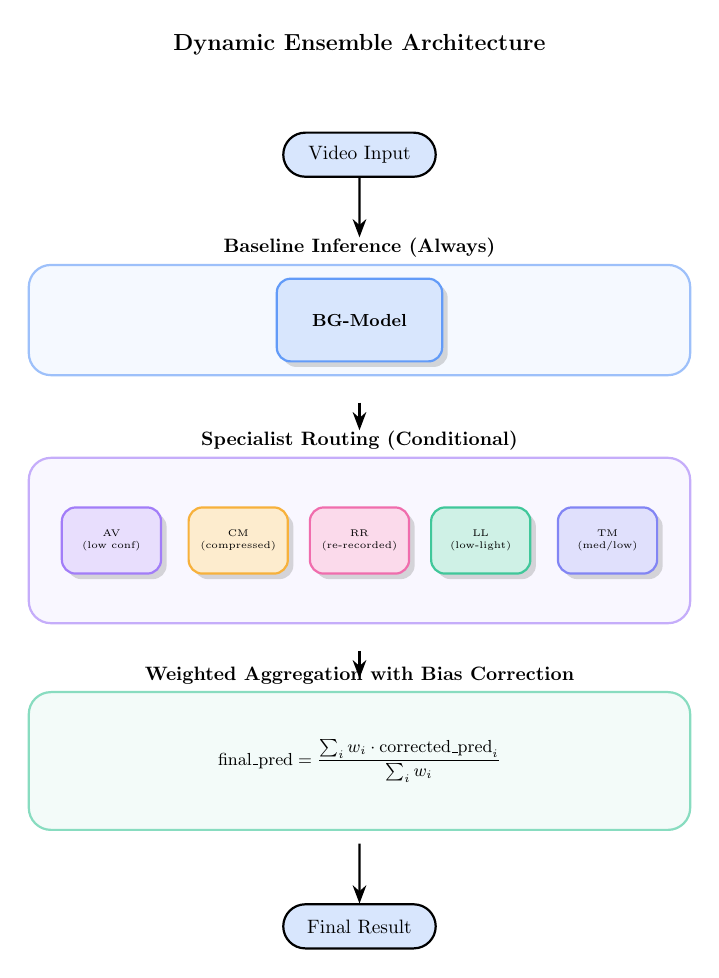
\begin{tikzpicture}[scale=0.7, transform shape]
    
    % Title
    \node[font=\large\bfseries] at (0,10) {Dynamic Ensemble Architecture};
    
    % Video Input
    \node[startstop, minimum width=3cm] (input) at (0,8) {Video Input};
    
    % Baseline Inference
    \begin{scope}[shift={(0,5)}]
        \node[container=bgModelColor, minimum width=12cm, minimum height=2cm] (basebox) {};
        \node[above, font=\bfseries] at (basebox.north) {Baseline Inference (Always)};
        \node[bgmodel, minimum width=3cm] at (0,0) {BG-Model};
    \end{scope}
    
    % Specialist Routing
    \begin{scope}[shift={(0,1)}]
        \node[container=erakshaSecondary, minimum width=12cm, minimum height=3cm] (specbox) {};
        \node[above, font=\bfseries] at (specbox.north) {Specialist Routing (Conditional)};
        
        \node[avmodel, minimum width=1.8cm, minimum height=1.2cm, font=\tiny] at (-4.5,0) {AV\\(low conf)};
        \node[cmmodel, minimum width=1.8cm, minimum height=1.2cm, font=\tiny] at (-2.2,0) {CM\\(compressed)};
        \node[rrmodel, minimum width=1.8cm, minimum height=1.2cm, font=\tiny] at (0,0) {RR\\(re-recorded)};
        \node[llmodel, minimum width=1.8cm, minimum height=1.2cm, font=\tiny] at (2.2,0) {LL\\(low-light)};
        \node[tmmodel, minimum width=1.8cm, minimum height=1.2cm, font=\tiny] at (4.5,0) {TM\\(med/low)};
    \end{scope}
    
    % Weighted Aggregation
    \begin{scope}[shift={(0,-3)}]
        \node[container=erakshaAccent, minimum width=12cm, minimum height=2.5cm] (aggbox) {};
        \node[above, font=\bfseries] at (aggbox.north) {Weighted Aggregation with Bias Correction};
        
        \node[font=\small] at (0,0) {$\displaystyle \text{final\_pred} = \frac{\sum_{i} w_i \cdot \text{corrected\_pred}_i}{\sum_{i} w_i}$};
    \end{scope}
    
    % Output
    \node[startstop, minimum width=3cm] (output) at (0,-6) {Final Result};
    
    % Arrows
    \draw[arrow] (input) -- (0,6.5);
    \draw[arrow] (0,3.5) -- (0,3);
    \draw[arrow] (0,-1) -- (0,-1.5);
    \draw[arrow] (0,-4.5) -- (output);
    
\end{tikzpicture}
\caption{Dynamic Ensemble with Conditional Specialist Routing}
\label{fig:ensemble}
\end{figure}

\subsection{Model Weight Configuration}

\begin{figure}[H]
\centering
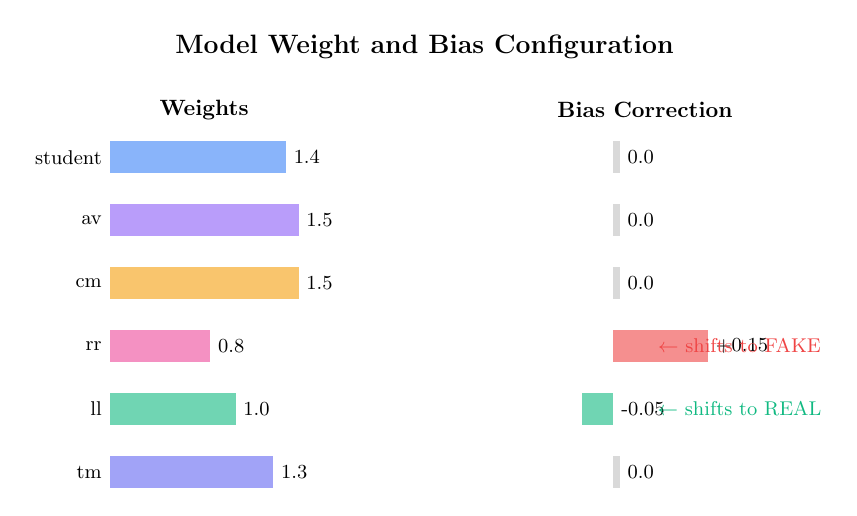
\begin{tikzpicture}[scale=0.8, transform shape]
    
    % Title
    \node[font=\large\bfseries] at (0,6) {Model Weight and Bias Configuration};
    
    % Weight bars
    \begin{scope}[shift={(-5,0)}]
        % Student
        \fill[bgModelColor!60] (0,4) rectangle (2.8,4.5);
        \node[left] at (0,4.25) {\small student};
        \node[right] at (2.8,4.25) {\small 1.4};
        
        % AV
        \fill[avModelColor!60] (0,3) rectangle (3,3.5);
        \node[left] at (0,3.25) {\small av};
        \node[right] at (3,3.25) {\small 1.5};
        
        % CM
        \fill[cmModelColor!60] (0,2) rectangle (3,2.5);
        \node[left] at (0,2.25) {\small cm};
        \node[right] at (3,2.25) {\small 1.5};
        
        % RR
        \fill[rrModelColor!60] (0,1) rectangle (1.6,1.5);
        \node[left] at (0,1.25) {\small rr};
        \node[right] at (1.6,1.25) {\small 0.8};
        
        % LL
        \fill[llModelColor!60] (0,0) rectangle (2,0.5);
        \node[left] at (0,0.25) {\small ll};
        \node[right] at (2,0.25) {\small 1.0};
        
        % TM
        \fill[tmModelColor!60] (0,-1) rectangle (2.6,-0.5);
        \node[left] at (0,-0.75) {\small tm};
        \node[right] at (2.6,-0.75) {\small 1.3};
        
        \node[font=\bfseries] at (1.5,5) {Weights};
    \end{scope}
    
    % Bias correction bars
    \begin{scope}[shift={(3,0)}]
        % Student
        \fill[gray!30] (0,4) rectangle (0.1,4.5);
        \node[right] at (0.1,4.25) {\small 0.0};
        
        % AV
        \fill[gray!30] (0,3) rectangle (0.1,3.5);
        \node[right] at (0.1,3.25) {\small 0.0};
        
        % CM
        \fill[gray!30] (0,2) rectangle (0.1,2.5);
        \node[right] at (0.1,2.25) {\small 0.0};
        
        % RR (positive)
        \fill[erakshaDanger!60] (0,1) rectangle (1.5,1.5);
        \node[right] at (1.5,1.25) {\small +0.15};
        
        % LL (negative)
        \fill[erakshaAccent!60] (-0.5,0) rectangle (0,0.5);
        \node[right] at (0,0.25) {\small -0.05};
        
        % TM
        \fill[gray!30] (0,-1) rectangle (0.1,-0.5);
        \node[right] at (0.1,-0.75) {\small 0.0};
        
        \node[font=\bfseries] at (0.5,5) {Bias Correction};
    \end{scope}
    
    % Legend
    \node[font=\small, text=erakshaDanger] at (5,1.25) {$\leftarrow$ shifts to FAKE};
    \node[font=\small, text=erakshaAccent] at (5,0.25) {$\leftarrow$ shifts to REAL};
    
\end{tikzpicture}
\caption{Model Weight and Bias Correction Configuration}
\label{fig:weights}
\end{figure}

\subsection{Bias Correction Visualization}

\begin{figure}[H]
\centering
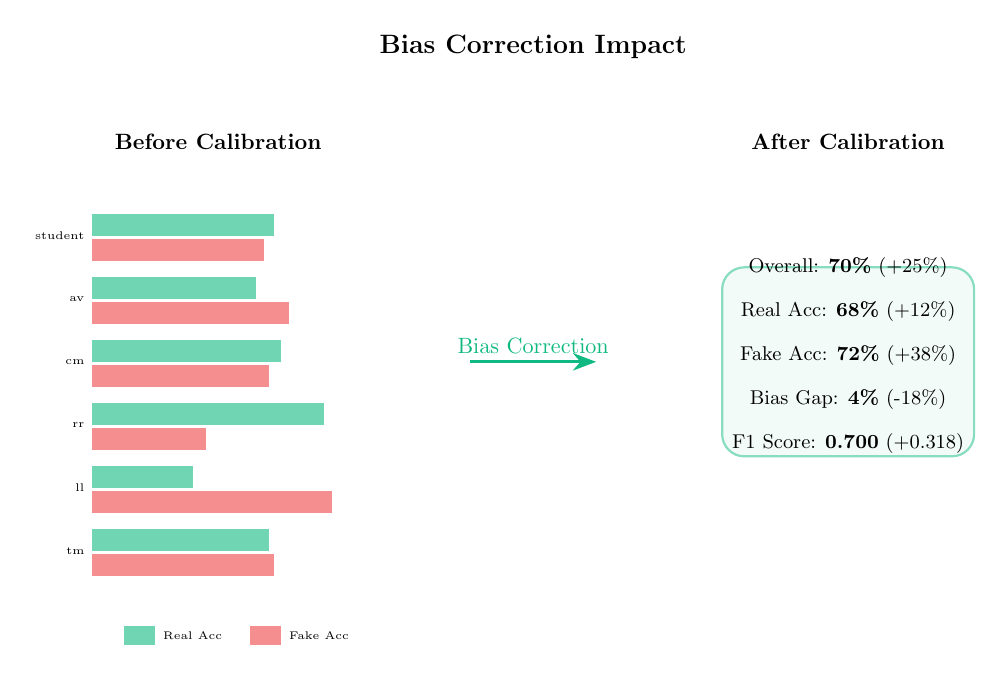
\begin{tikzpicture}[scale=0.8, transform shape]
    
    % Title
    \node[font=\large\bfseries] at (0,7) {Bias Correction Impact};
    
    % Before calibration
    \begin{scope}[shift={(-5,0)}]
        \node[font=\bfseries] at (0,5.5) {Before Calibration};
        
        % Accuracy bars
        \foreach \model/\real/\fake/\y in {
            student/72/68/4,
            av/65/78/3,
            cm/75/70/2,
            rr/92/45/1,
            ll/40/95/0,
            tm/70/72/-1
        } {
            % Real accuracy (green)
            \pgfmathsetmacro{\realwidth}{\real/25}
            \fill[erakshaAccent!60] (-2,\y) rectangle (-2+\realwidth,\y+0.35);
            
            % Fake accuracy (red)
            \pgfmathsetmacro{\fakewidth}{\fake/25}
            \fill[erakshaDanger!60] (-2,\y-0.4) rectangle (-2+\fakewidth,\y-0.05);
            
            \node[left, font=\tiny] at (-2,\y) {\model};
        }
        
        % Legend
        \fill[erakshaAccent!60] (-1.5,-2.5) rectangle (-1,-2.2);
        \node[right, font=\tiny] at (-1,-2.35) {Real Acc};
        \fill[erakshaDanger!60] (0.5,-2.5) rectangle (1,-2.2);
        \node[right, font=\tiny] at (1,-2.35) {Fake Acc};
    \end{scope}
    
    % After calibration
    \begin{scope}[shift={(5,0)}]
        \node[font=\bfseries] at (0,5.5) {After Calibration};
        
        % Improved metrics
        \node[container=erakshaAccent, minimum width=4cm, minimum height=3cm] at (0,2) {};
        
        \node[font=\small] at (0,3.5) {Overall: \textbf{70\%} (+25\%)};
        \node[font=\small] at (0,2.8) {Real Acc: \textbf{68\%} (+12\%)};
        \node[font=\small] at (0,2.1) {Fake Acc: \textbf{72\%} (+38\%)};
        \node[font=\small] at (0,1.4) {Bias Gap: \textbf{4\%} (-18\%)};
        \node[font=\small] at (0,0.7) {F1 Score: \textbf{0.700} (+0.318)};
    \end{scope}
    
    % Arrow
    \draw[arrow, very thick, erakshaAccent] (-1,2) -- node[above] {Bias Correction} (1,2);
    
\end{tikzpicture}
\caption{Bias Correction Impact on Model Performance}
\label{fig:bias-correction}
\end{figure}

\subsection{Decision Boundaries}

\begin{figure}[H]
\centering
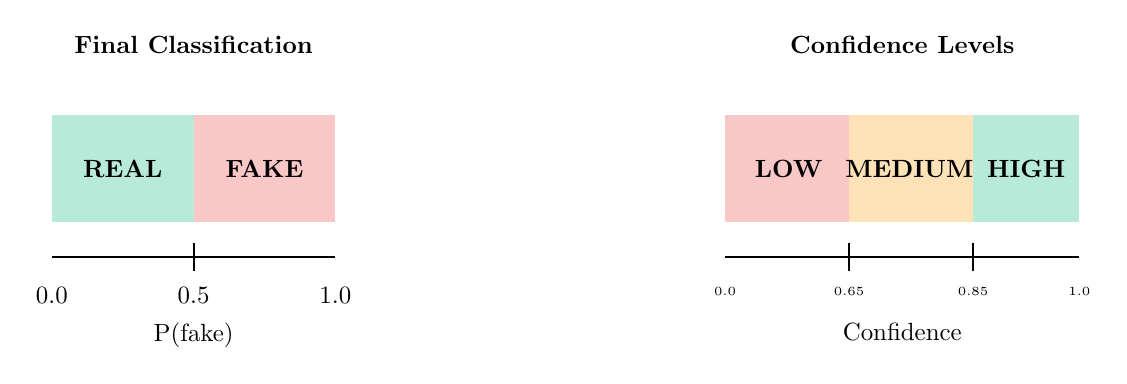
\begin{tikzpicture}[scale=0.9, transform shape]
    
    % Classification boundary
    \begin{scope}[shift={(-5,0)}]
        \node[font=\bfseries] at (0,3) {Final Classification};
        
        \draw[thick] (-2,0) -- (2,0);
        \draw[thick] (0,-0.2) -- (0,0.2);
        
        \fill[erakshaDanger!30] (0,0.5) rectangle (2,2);
        \fill[erakshaAccent!30] (-2,0.5) rectangle (0,2);
        
        \node at (1,1.25) {\textbf{FAKE}};
        \node at (-1,1.25) {\textbf{REAL}};
        
        \node[below] at (0,-0.3) {0.5};
        \node[below] at (-2,-0.3) {0.0};
        \node[below] at (2,-0.3) {1.0};
        \node[below] at (0,-0.8) {P(fake)};
    \end{scope}
    
    % Confidence levels
    \begin{scope}[shift={(5,0)}]
        \node[font=\bfseries] at (0,3) {Confidence Levels};
        
        \draw[thick] (-2.5,0) -- (2.5,0);
        
        \fill[erakshaDanger!30] (-2.5,0.5) rectangle (-0.75,2);
        \fill[erakshaWarning!30] (-0.75,0.5) rectangle (1,2);
        \fill[erakshaAccent!30] (1,0.5) rectangle (2.5,2);
        
        \node at (-1.6,1.25) {\textbf{LOW}};
        \node at (0.1,1.25) {\textbf{MEDIUM}};
        \node at (1.75,1.25) {\textbf{HIGH}};
        
        \draw[thick] (-0.75,-0.2) -- (-0.75,0.2);
        \draw[thick] (1,-0.2) -- (1,0.2);
        
        \node[below, font=\tiny] at (-0.75,-0.3) {0.65};
        \node[below, font=\tiny] at (1,-0.3) {0.85};
        \node[below, font=\tiny] at (-2.5,-0.3) {0.0};
        \node[below, font=\tiny] at (2.5,-0.3) {1.0};
        \node[below] at (0,-0.8) {Confidence};
    \end{scope}
    
\end{tikzpicture}
\caption{Classification and Confidence Decision Boundaries}
\label{fig:decision-boundaries}
\end{figure}

\newpage

%%%%%%%%%%%%%%%%%%%%%%%%%%%%%%%%%%%%%%%%%%%%%%%%%%%%%%%%%%%%%%%%%%%%%%%%%%%%%%%
%% SECTION 5: PREPROCESSING PIPELINE
%%%%%%%%%%%%%%%%%%%%%%%%%%%%%%%%%%%%%%%%%%%%%%%%%%%%%%%%%%%%%%%%%%%%%%%%%%%%%%%
\section{Preprocessing Pipeline}

\subsection{Complete Preprocessing Flow}

\begin{figure}[H]
\centering
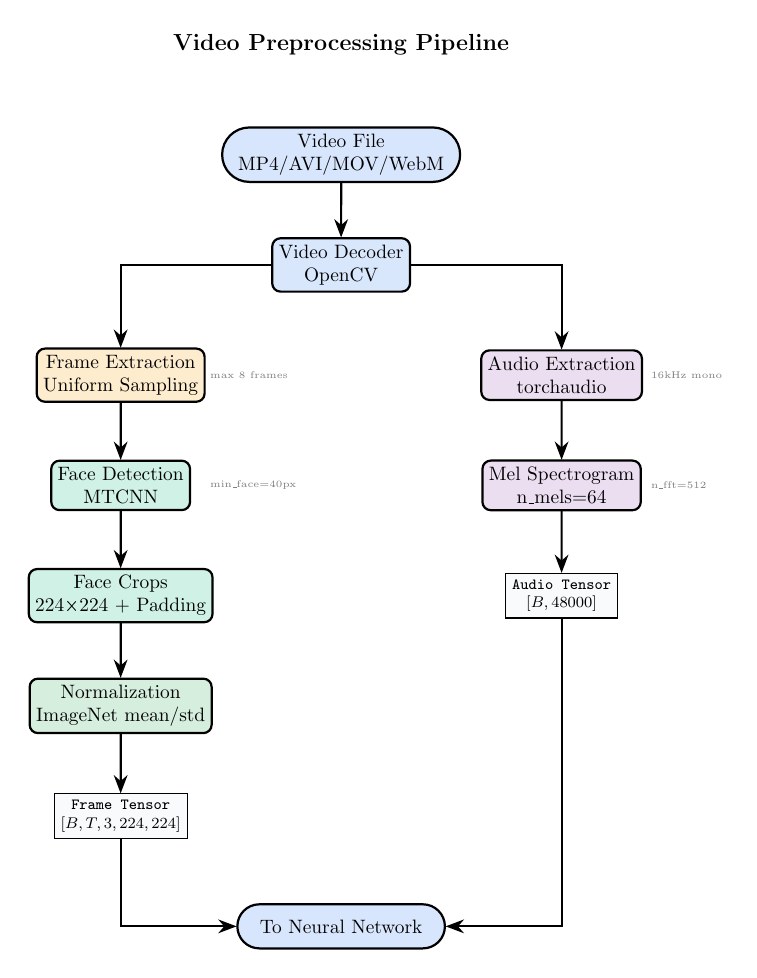
\begin{tikzpicture}[scale=0.7, transform shape, node distance=1cm]
    
    % Title
    \node[font=\large\bfseries] at (0,9) {Video Preprocessing Pipeline};
    
    % Video Input
    \node[startstop, minimum width=3cm] (input) at (0,7) {Video File\\MP4/AVI/MOV/WebM};
    
    % Video Decoder
    \node[process, fill=convColor!20] (decoder) at (0,5) {Video Decoder\\OpenCV};
    
    % Parallel branches
    \node[process, fill=erakshaWarning!20] (frameext) at (-4,3) {Frame Extraction\\Uniform Sampling};
    \node[process, fill=fcColor!20] (audioext) at (4,3) {Audio Extraction\\torchaudio};
    
    % Face Detection
    \node[process, fill=erakshaAccent!20] (facedet) at (-4,1) {Face Detection\\MTCNN};
    
    % Mel Spectrogram
    \node[process, fill=fcColor!20] (mel) at (4,1) {Mel Spectrogram\\n\_mels=64};
    
    % Face Crops
    \node[process, fill=erakshaAccent!20] (crops) at (-4,-1) {Face Crops\\224×224 + Padding};
    
    % Audio Features
    \node[tensor] (audiofeat) at (4,-1) {Audio Tensor\\$[B, 48000]$};
    
    % Normalization
    \node[process, fill=bnColor!20] (norm) at (-4,-3) {Normalization\\ImageNet mean/std};
    
    % Frame Tensor
    \node[tensor] (frametensor) at (-4,-5) {Frame Tensor\\$[B, T, 3, 224, 224]$};
    
    % To Model
    \node[startstop, minimum width=4cm] (tomodel) at (0,-7) {To Neural Network};
    
    % Arrows
    \draw[arrow] (input) -- (decoder);
    \draw[arrow] (decoder) -| (frameext);
    \draw[arrow] (decoder) -| (audioext);
    \draw[arrow] (frameext) -- (facedet);
    \draw[arrow] (audioext) -- (mel);
    \draw[arrow] (facedet) -- (crops);
    \draw[arrow] (mel) -- (audiofeat);
    \draw[arrow] (crops) -- (norm);
    \draw[arrow] (norm) -- (frametensor);
    \draw[arrow] (frametensor) |- (tomodel);
    \draw[arrow] (audiofeat) |- (tomodel);
    
    % Annotations
    \node[font=\tiny, text=gray, right] at (-2.5,3) {max 8 frames};
    \node[font=\tiny, text=gray, right] at (5.5,3) {16kHz mono};
    \node[font=\tiny, text=gray, right] at (-2.5,1) {min\_face=40px};
    \node[font=\tiny, text=gray, right] at (5.5,1) {n\_fft=512};
    
\end{tikzpicture}
\caption{Complete Video Preprocessing Pipeline}
\label{fig:preprocessing}
\end{figure}

\subsection{MTCNN Face Detection Pipeline}

\begin{figure}[H]
\centering
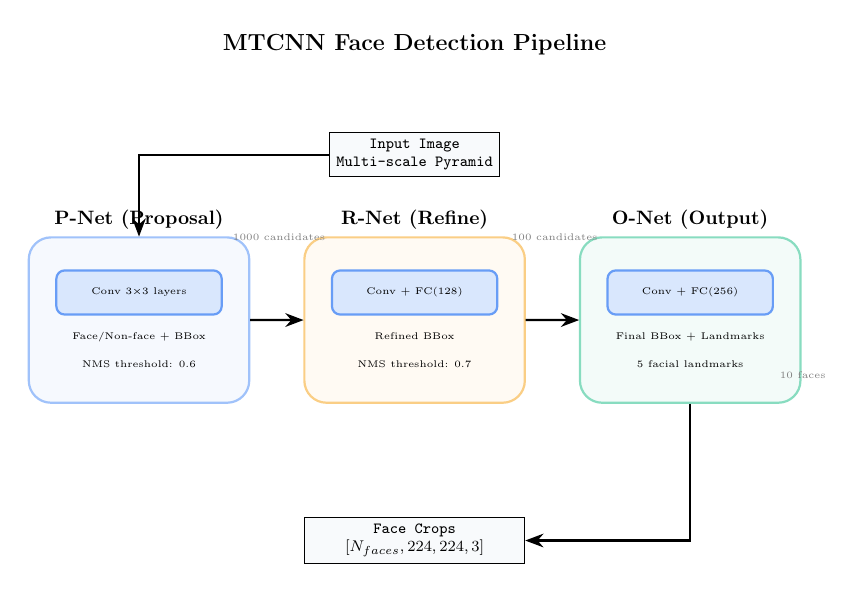
\begin{tikzpicture}[scale=0.7, transform shape, node distance=1cm]
    
    % Title
    \node[font=\large\bfseries] at (0,9) {MTCNN Face Detection Pipeline};
    
    % Input
    \node[tensor, minimum width=3cm] (input) at (0,7) {Input Image\\Multi-scale Pyramid};
    
    % P-Net
    \begin{scope}[shift={(-5,4)}]
        \node[container=convColor, minimum width=4cm, minimum height=3cm] (pnet) {};
        \node[above, font=\bfseries] at (pnet.north) {P-Net (Proposal)};
        \node[convlayer, minimum width=3cm, font=\tiny] at (0,0.5) {Conv 3×3 layers};
        \node[font=\tiny] at (0,-0.3) {Face/Non-face + BBox};
        \node[font=\tiny] at (0,-0.8) {NMS threshold: 0.6};
    \end{scope}
    
    % R-Net
    \begin{scope}[shift={(0,4)}]
        \node[container=erakshaWarning, minimum width=4cm, minimum height=3cm] (rnet) {};
        \node[above, font=\bfseries] at (rnet.north) {R-Net (Refine)};
        \node[convlayer, minimum width=3cm, font=\tiny] at (0,0.5) {Conv + FC(128)};
        \node[font=\tiny] at (0,-0.3) {Refined BBox};
        \node[font=\tiny] at (0,-0.8) {NMS threshold: 0.7};
    \end{scope}
    
    % O-Net
    \begin{scope}[shift={(5,4)}]
        \node[container=erakshaAccent, minimum width=4cm, minimum height=3cm] (onet) {};
        \node[above, font=\bfseries] at (onet.north) {O-Net (Output)};
        \node[convlayer, minimum width=3cm, font=\tiny] at (0,0.5) {Conv + FC(256)};
        \node[font=\tiny] at (0,-0.3) {Final BBox + Landmarks};
        \node[font=\tiny] at (0,-0.8) {5 facial landmarks};
    \end{scope}
    
    % Output
    \node[tensor, minimum width=4cm] (output) at (0,0) {Face Crops\\$[N_{faces}, 224, 224, 3]$};
    
    % Arrows
    \draw[arrow] (input) -| (pnet);
    \draw[arrow] (pnet) -- (rnet);
    \draw[arrow] (rnet) -- (onet);
    \draw[arrow] (onet) |- (output);
    
    % Candidate counts
    \node[font=\tiny, text=gray] at (-2.5,5.5) {~1000 candidates};
    \node[font=\tiny, text=gray] at (2.5,5.5) {~100 candidates};
    \node[font=\tiny, text=gray] at (7,3) {~10 faces};
    
\end{tikzpicture}
\caption{MTCNN Three-Stage Face Detection Pipeline}
\label{fig:mtcnn}
\end{figure}

\subsection{Mel Spectrogram Computation}

\begin{figure}[H]
\centering
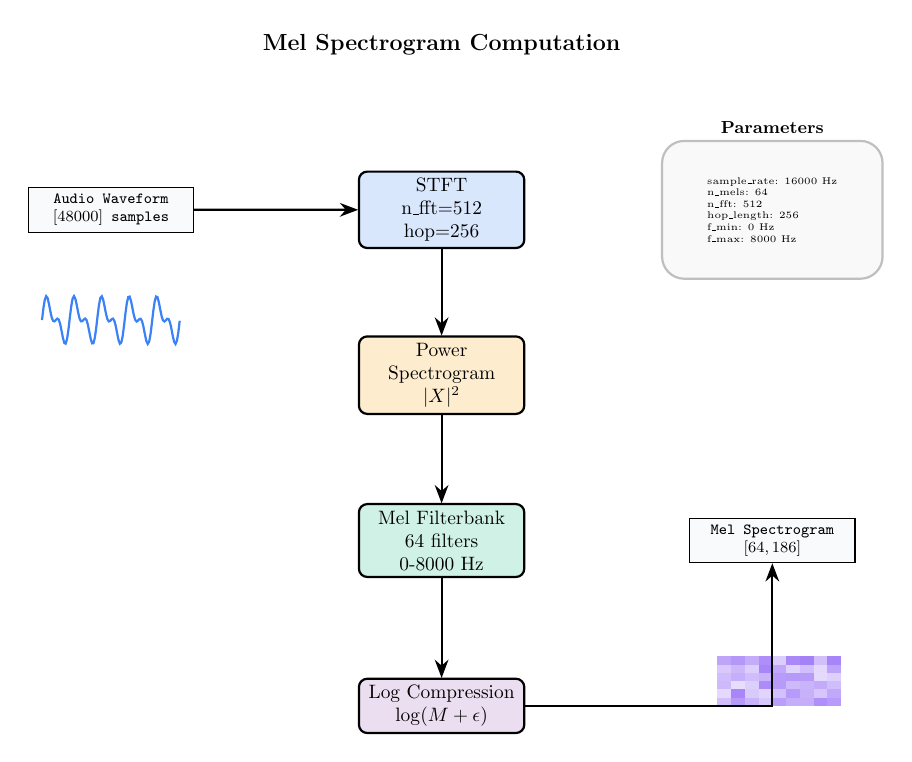
\begin{tikzpicture}[scale=0.7, transform shape]
    
    % Title
    \node[font=\large\bfseries] at (0,7) {Mel Spectrogram Computation};
    
    % Audio waveform
    \begin{scope}[shift={(-6,4)}]
        \node[tensor, minimum width=3cm] (audio) {Audio Waveform\\$[48000]$ samples};
        
        % Waveform visualization
        \draw[thick, erakshaPrimary] plot[domain=0:2.5, samples=100] 
            (\x-1.25, {0.3*sin(720*\x) + 0.2*sin(1440*\x) - 2});
    \end{scope}
    
    % STFT
    \begin{scope}[shift={(0,4)}]
        \node[process, fill=convColor!20, minimum width=3cm] (stft) {STFT\\n\_fft=512\\hop=256};
    \end{scope}
    
    % Power Spectrogram
    \begin{scope}[shift={(0,1)}]
        \node[process, fill=erakshaWarning!20, minimum width=3cm] (power) {Power\\Spectrogram\\$|X|^2$};
    \end{scope}
    
    % Mel Filterbank
    \begin{scope}[shift={(0,-2)}]
        \node[process, fill=erakshaAccent!20, minimum width=3cm] (mel) {Mel Filterbank\\64 filters\\0-8000 Hz};
    \end{scope}
    
    % Log compression
    \begin{scope}[shift={(0,-5)}]
        \node[process, fill=fcColor!20, minimum width=3cm] (log) {Log Compression\\$\log(M + \epsilon)$};
    \end{scope}
    
    % Output
    \begin{scope}[shift={(6,-2)}]
        \node[tensor, minimum width=3cm] (output) {Mel Spectrogram\\$[64, 186]$};
        
        % Spectrogram visualization
        \foreach \y in {0,...,5} {
            \foreach \x in {0,...,8} {
                \pgfmathsetmacro{\intensity}{rnd*60+20}
                \fill[erakshaSecondary!\intensity] (\x*0.25-1, \y*0.15-3) rectangle (\x*0.25-0.75, \y*0.15-2.85);
            }
        }
    \end{scope}
    
    % Arrows
    \draw[arrow] (audio) -- (stft);
    \draw[arrow] (stft) -- (power);
    \draw[arrow] (power) -- (mel);
    \draw[arrow] (mel) -- (log);
    \draw[arrow] (log) -| (output);
    
    % Parameters box
    \begin{scope}[shift={(6,4)}]
        \node[container=gray, minimum width=4cm, minimum height=2.5cm] (params) {};
        \node[above, font=\bfseries\small] at (params.north) {Parameters};
        \node[font=\tiny, align=left] at (0,0) {
            sample\_rate: 16000 Hz\\
            n\_mels: 64\\
            n\_fft: 512\\
            hop\_length: 256\\
            f\_min: 0 Hz\\
            f\_max: 8000 Hz
        };
    \end{scope}
    
\end{tikzpicture}
\caption{Mel Spectrogram Computation Pipeline}
\label{fig:mel-spectrogram}
\end{figure}

\newpage

%%%%%%%%%%%%%%%%%%%%%%%%%%%%%%%%%%%%%%%%%%%%%%%%%%%%%%%%%%%%%%%%%%%%%%%%%%%%%%%
%% SECTION 6: INFERENCE ENGINE
%%%%%%%%%%%%%%%%%%%%%%%%%%%%%%%%%%%%%%%%%%%%%%%%%%%%%%%%%%%%%%%%%%%%%%%%%%%%%%%
\section{Inference Engine}

\subsection{Complete Inference Pipeline}

\begin{figure}[H]
\centering
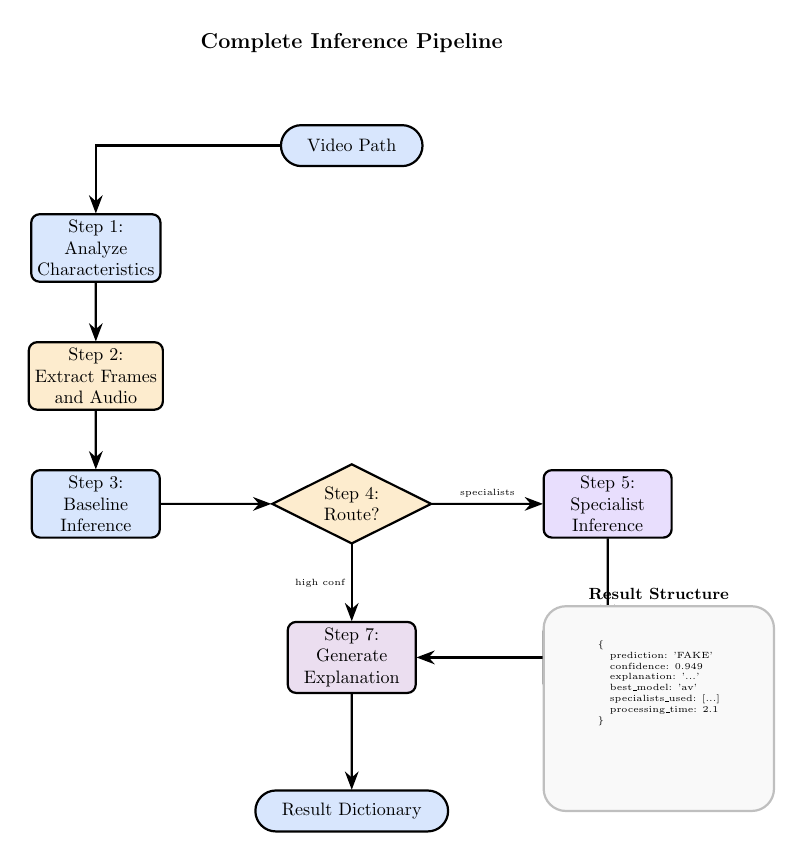
\begin{tikzpicture}[scale=0.65, transform shape, node distance=0.8cm]
    
    % Title
    \node[font=\large\bfseries] at (0,12) {Complete Inference Pipeline};
    
    % Steps
    \node[startstop, minimum width=3cm] (start) at (0,10) {Video Path};
    
    \node[process, fill=convColor!20] (step1) at (-5,8) {Step 1:\\Analyze\\Characteristics};
    
    \node[process, fill=erakshaWarning!20] (step2) at (-5,5.5) {Step 2:\\Extract Frames\\and Audio};
    
    \node[process, fill=bgModelColor!20] (step3) at (-5,3) {Step 3:\\Baseline\\Inference};
    
    \node[decision] (step4) at (0,3) {Step 4:\\Route?};
    
    \node[process, fill=erakshaSecondary!20] (step5) at (5,3) {Step 5:\\Specialist\\Inference};
    
    \node[process, fill=erakshaAccent!20] (step6) at (5,0) {Step 6:\\Aggregate\\Predictions};
    
    \node[process, fill=fcColor!20] (step7) at (0,0) {Step 7:\\Generate\\Explanation};
    
    \node[startstop, minimum width=4cm] (end) at (0,-3) {Result Dictionary};
    
    % Arrows
    \draw[arrow] (start) -| (step1);
    \draw[arrow] (step1) -- (step2);
    \draw[arrow] (step2) -- (step3);
    \draw[arrow] (step3) -- (step4);
    \draw[arrow] (step4) -- node[above, font=\tiny] {specialists} (step5);
    \draw[arrow] (step4) -- node[left, font=\tiny] {high conf} (step7);
    \draw[arrow] (step5) -- (step6);
    \draw[arrow] (step6) -- (step7);
    \draw[arrow] (step7) -- (end);
    
    % Result structure
    \begin{scope}[shift={(6,-1)}]
        \node[container=gray, minimum width=4.5cm, minimum height=4cm] (result) {};
        \node[above, font=\bfseries\small] at (result.north) {Result Structure};
        \node[font=\tiny, align=left] at (0,0.5) {
            \texttt{\{}\\
            \quad prediction: 'FAKE'\\
            \quad confidence: 0.949\\
            \quad explanation: '...'\\
            \quad best\_model: 'av'\\
            \quad specialists\_used: [...]\\
            \quad processing\_time: 2.1\\
            \texttt{\}}
        };
    \end{scope}
    
\end{tikzpicture}
\caption{Complete Inference Pipeline with 7 Steps}
\label{fig:inference-pipeline}
\end{figure}

\subsection{Streaming Inference Architecture}

\begin{figure}[H]
\centering
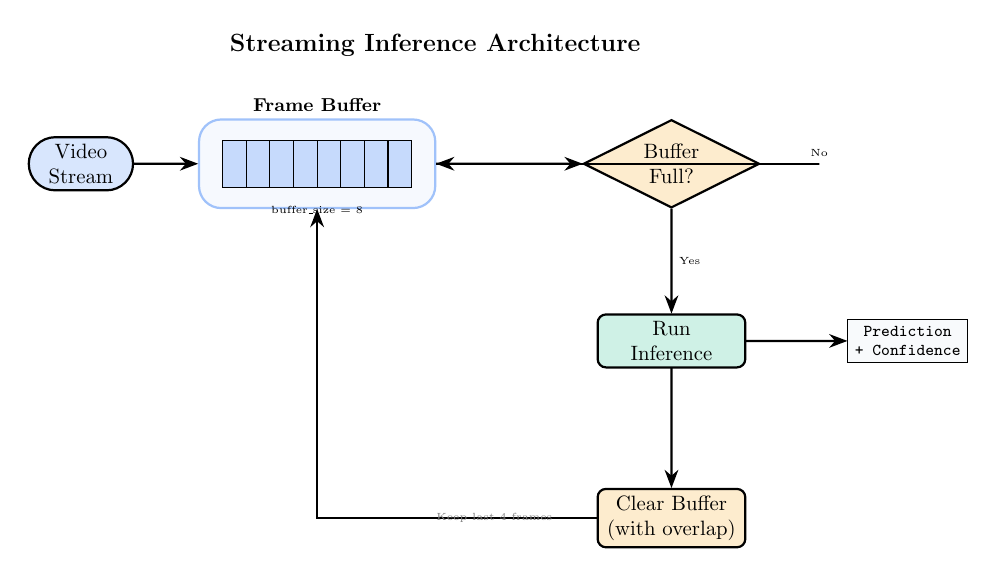
\begin{tikzpicture}[scale=0.75, transform shape]
    
    % Title
    \node[font=\large\bfseries] at (0,7) {Streaming Inference Architecture};
    
    % Video Stream
    \node[startstop] (stream) at (-6,5) {Video\\Stream};
    
    % Frame Buffer
    \begin{scope}[shift={(-2,5)}]
        \node[container=convColor, minimum width=4cm, minimum height=1.5cm] (buffer) {};
        \node[above, font=\bfseries\small] at (buffer.north) {Frame Buffer};
        
        % Buffer slots
        \foreach \i in {0,...,7} {
            \node[draw, minimum width=0.4cm, minimum height=0.8cm, fill=convColor!30] at (-1.4+\i*0.4,0) {};
        }
        \node[below, font=\tiny] at (0,-0.6) {buffer\_size = 8};
    \end{scope}
    
    % Check buffer
    \node[decision, minimum width=2cm] (check) at (4,5) {Buffer\\Full?};
    
    % Process
    \node[process, fill=erakshaAccent!20] (process) at (4,2) {Run\\Inference};
    
    % Clear buffer
    \node[process, fill=erakshaWarning!20] (clear) at (4,-1) {Clear Buffer\\(with overlap)};
    
    % Output
    \node[tensor] (output) at (8,2) {Prediction\\+ Confidence};
    
    % Arrows
    \draw[arrow] (stream) -- (buffer);
    \draw[arrow] (buffer) -- (check);
    \draw[arrow] (check) -- node[right, font=\tiny] {Yes} (process);
    \draw[arrow] (check.east) -- ++(1,0) |- node[above, font=\tiny, pos=0.25] {No} (buffer.east);
    \draw[arrow] (process) -- (output);
    \draw[arrow] (process) -- (clear);
    \draw[arrow] (clear) -| (buffer);
    
    % Overlap annotation
    \node[font=\tiny, text=gray] at (1,-1) {Keep last 4 frames};
    
\end{tikzpicture}
\caption{Streaming Inference with Frame Buffer}
\label{fig:streaming}
\end{figure}

\subsection{Memory Optimization Strategies}

\begin{figure}[H]
\centering
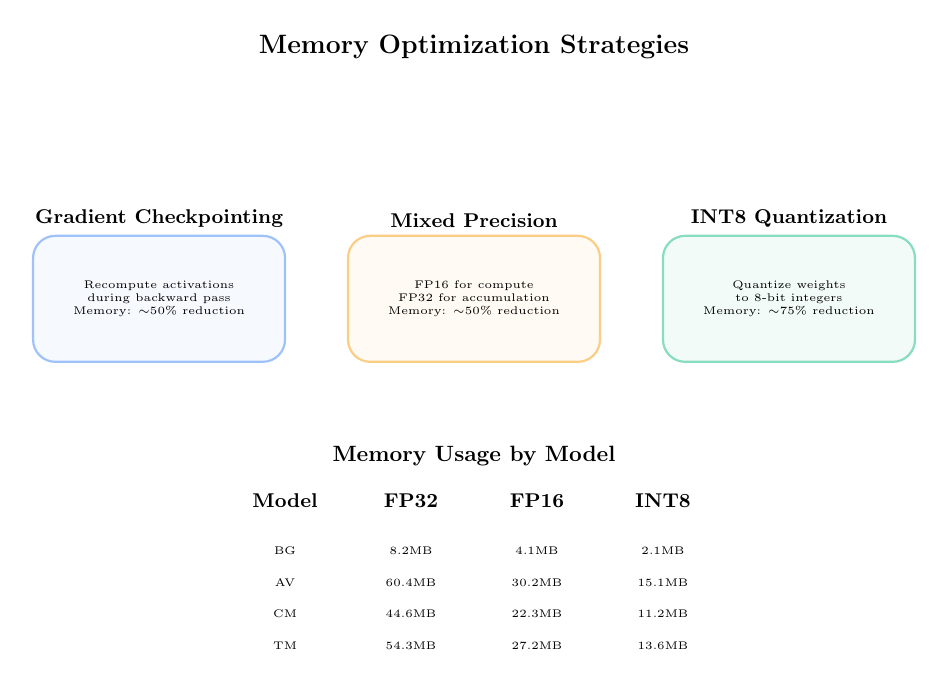
\begin{tikzpicture}[scale=0.8, transform shape]
    
    % Title
    \node[font=\large\bfseries] at (0,6) {Memory Optimization Strategies};
    
    % Strategies
    \begin{scope}[shift={(-5,2)}]
        \node[container=convColor, minimum width=4cm, minimum height=2cm] (gc) {};
        \node[above, font=\bfseries\small] at (gc.north) {Gradient Checkpointing};
        \node[font=\tiny, align=center] at (0,0) {Recompute activations\\during backward pass\\Memory: $\sim$50\% reduction};
    \end{scope}
    
    \begin{scope}[shift={(0,2)}]
        \node[container=erakshaWarning, minimum width=4cm, minimum height=2cm] (mp) {};
        \node[above, font=\bfseries\small] at (mp.north) {Mixed Precision};
        \node[font=\tiny, align=center] at (0,0) {FP16 for compute\\FP32 for accumulation\\Memory: $\sim$50\% reduction};
    \end{scope}
    
    \begin{scope}[shift={(5,2)}]
        \node[container=erakshaAccent, minimum width=4cm, minimum height=2cm] (quant) {};
        \node[above, font=\bfseries\small] at (quant.north) {INT8 Quantization};
        \node[font=\tiny, align=center] at (0,0) {Quantize weights\\to 8-bit integers\\Memory: $\sim$75\% reduction};
    \end{scope}
    
    % Memory comparison
    \begin{scope}[shift={(0,-2)}]
        \node[font=\bfseries] at (0,1.5) {Memory Usage by Model};
        
        % Table header
        \node[font=\small\bfseries] at (-3,0.8) {Model};
        \node[font=\small\bfseries] at (-1,0.8) {FP32};
        \node[font=\small\bfseries] at (1,0.8) {FP16};
        \node[font=\small\bfseries] at (3,0.8) {INT8};
        
        % Data rows
        \foreach \model/\fp/\fph/\int/\y in {
            BG/8.2/4.1/2.1/0,
            AV/60.4/30.2/15.1/-0.5,
            CM/44.6/22.3/11.2/-1,
            TM/54.3/27.2/13.6/-1.5
        } {
            \node[font=\tiny] at (-3,\y) {\model};
            \node[font=\tiny] at (-1,\y) {\fp MB};
            \node[font=\tiny] at (1,\y) {\fph MB};
            \node[font=\tiny] at (3,\y) {\int MB};
        }
    \end{scope}
    
\end{tikzpicture}
\caption{Memory Optimization Strategies and Comparison}
\label{fig:memory-optimization}
\end{figure}

\subsection{Latency Breakdown}

\begin{figure}[H]
\centering
\begin{tikzpicture}[scale=0.9, transform shape]
    
    % Title
    \node[font=\large\bfseries] at (0,5) {Latency Breakdown (per video)};
    
    % Pie chart style breakdown
    \begin{scope}[shift={(-4,0)}]
        % Bars
        \fill[convColor!60] (0,3) rectangle (1.5,3.4);
        \node[right, font=\tiny] at (1.6,3.2) {Video Loading: 150ms (7\%)};
        
        \fill[erakshaWarning!60] (0,2.4) rectangle (2,2.8);
        \node[right, font=\tiny] at (2.1,2.6) {Frame Extraction: 200ms (10\%)};
        
        \fill[erakshaDanger!60] (0,1.8) rectangle (3,2.2);
        \node[right, font=\tiny] at (3.1,2) {Face Detection: 300ms (14\%)};
        
        \fill[fcColor!60] (0,1.2) rectangle (1,1.6);
        \node[right, font=\tiny] at (1.1,1.4) {Audio Extraction: 100ms (5\%)};
        
        \fill[bgModelColor!60] (0,0.6) rectangle (1.5,1);
        \node[right, font=\tiny] at (1.6,0.8) {Baseline Inference: 150ms (7\%)};
        
        \fill[erakshaSecondary!60] (0,0) rectangle (4,0.4);
        \node[right, font=\tiny] at (4.1,0.2) {Specialist Inference: 400ms (19\%)};
        
        \fill[erakshaAccent!60] (0,-0.6) rectangle (0.1,-0.2);
        \node[right, font=\tiny] at (0.2,-0.4) {Aggregation: 10ms (<1\%)};
        
        \fill[gray!60] (0,-1.2) rectangle (0.2,-0.8);
        \node[right, font=\tiny] at (0.3,-1) {Explanation: 20ms (1\%)};
    \end{scope}
    
    % Total
    \node[container=erakshaPrimary, minimum width=4cm, minimum height=1.5cm] at (4,1) {};
    \node[font=\bfseries] at (4,1.3) {Total: 1330ms};
    \node[font=\small] at (4,0.7) {Target: $<$2000ms ✓};
    
\end{tikzpicture}
\caption{Latency Breakdown by Processing Stage}
\label{fig:latency}
\end{figure}

\newpage

%%%%%%%%%%%%%%%%%%%%%%%%%%%%%%%%%%%%%%%%%%%%%%%%%%%%%%%%%%%%%%%%%%%%%%%%%%%%%%%
%% SECTION 7: EXPLAINABILITY AND TRUST
%%%%%%%%%%%%%%%%%%%%%%%%%%%%%%%%%%%%%%%%%%%%%%%%%%%%%%%%%%%%%%%%%%%%%%%%%%%%%%%
\section{Explainability and Trust Mechanisms}

\subsection{Grad-CAM Visualization Pipeline}

\begin{figure}[H]
\centering
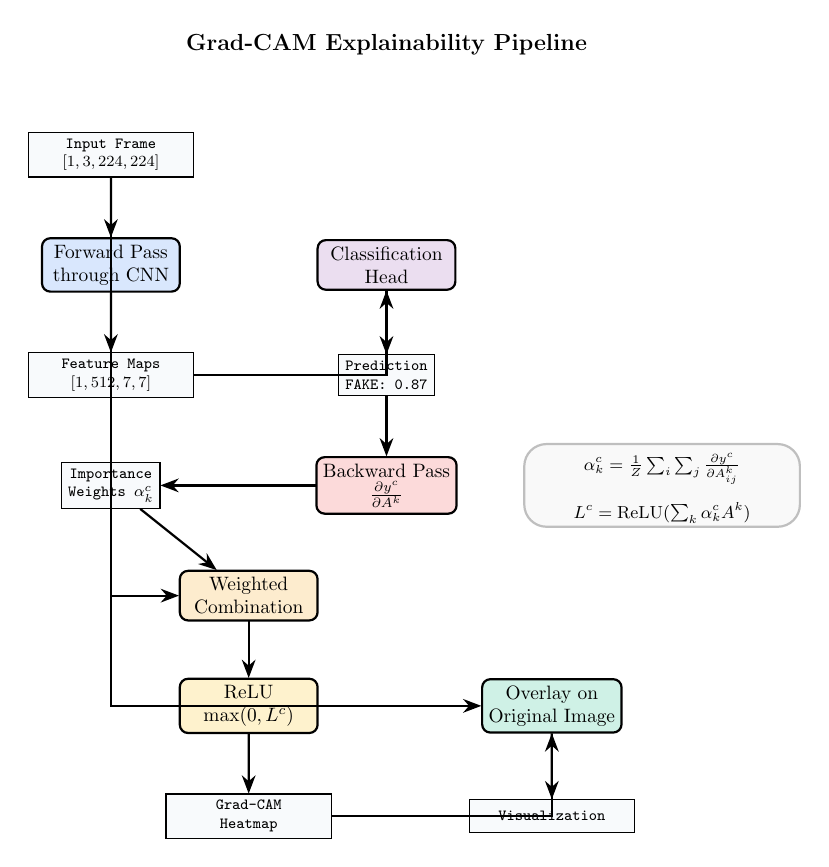
\begin{tikzpicture}[scale=0.7, transform shape, node distance=1cm]
    
    % Title
    \node[font=\large\bfseries] at (0,9) {Grad-CAM Explainability Pipeline};
    
    % Input
    \node[tensor, minimum width=3cm] (input) at (-5,7) {Input Frame\\$[1, 3, 224, 224]$};
    
    % Forward pass
    \node[process, fill=convColor!20] (forward) at (-5,5) {Forward Pass\\through CNN};
    
    % Feature maps
    \node[tensor, minimum width=3cm] (features) at (-5,3) {Feature Maps\\$[1, 512, 7, 7]$};
    
    % Classification
    \node[process, fill=fcColor!20] (classify) at (0,5) {Classification\\Head};
    
    % Prediction
    \node[tensor] (pred) at (0,3) {Prediction\\FAKE: 0.87};
    
    % Backward pass
    \node[process, fill=erakshaDanger!20] (backward) at (0,1) {Backward Pass\\$\frac{\partial y^c}{\partial A^k}$};
    
    % Weights
    \node[tensor] (weights) at (-5,1) {Importance\\Weights $\alpha_k^c$};
    
    % Weighted combination
    \node[process, fill=erakshaWarning!20] (combine) at (-2.5,-1) {Weighted\\Combination};
    
    % ReLU
    \node[process, fill=reluColor!20] (relu) at (-2.5,-3) {ReLU\\$\max(0, L^c)$};
    
    % Heatmap
    \node[tensor, minimum width=3cm] (heatmap) at (-2.5,-5) {Grad-CAM\\Heatmap};
    
    % Overlay
    \node[process, fill=erakshaAccent!20] (overlay) at (3,-3) {Overlay on\\Original Image};
    
    % Output
    \node[tensor, minimum width=3cm] (output) at (3,-5) {Visualization};
    
    % Arrows
    \draw[arrow] (input) -- (forward);
    \draw[arrow] (forward) -- (features);
    \draw[arrow] (features) -| (classify);
    \draw[arrow] (classify) -- (pred);
    \draw[arrow] (pred) -- (backward);
    \draw[arrow] (backward) -- (weights);
    \draw[arrow] (features) |- (combine);
    \draw[arrow] (weights) -- (combine);
    \draw[arrow] (combine) -- (relu);
    \draw[arrow] (relu) -- (heatmap);
    \draw[arrow] (heatmap) -| (overlay);
    \draw[arrow] (input) |- (overlay);
    \draw[arrow] (overlay) -- (output);
    
    % Formula
    \node[container=gray, minimum width=5cm, minimum height=1.5cm] at (5,1) {};
    \node[font=\small] at (5,1.3) {$\alpha_k^c = \frac{1}{Z}\sum_i\sum_j \frac{\partial y^c}{\partial A_{ij}^k}$};
    \node[font=\small] at (5,0.5) {$L^c = \text{ReLU}(\sum_k \alpha_k^c A^k)$};
    
\end{tikzpicture}
\caption{Grad-CAM Visualization Pipeline}
\label{fig:gradcam}
\end{figure}

\subsection{Facial Region Analysis}

\begin{figure}[H]
\centering
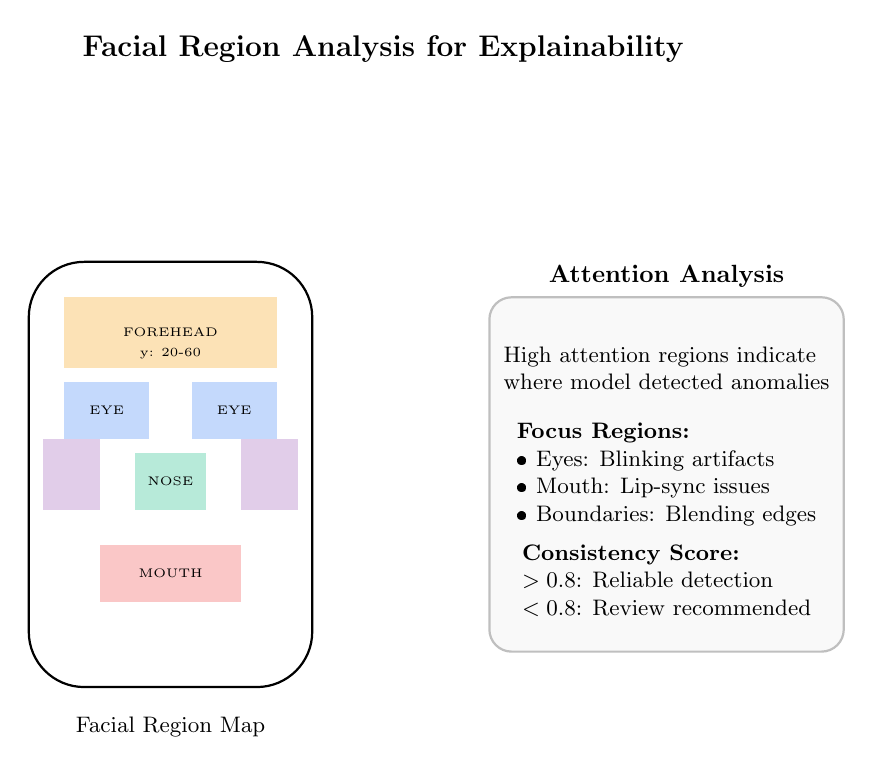
\begin{tikzpicture}[scale=0.9, transform shape]
    
    % Title
    \node[font=\large\bfseries] at (0,6) {Facial Region Analysis for Explainability};
    
    % Face outline
    \begin{scope}[shift={(-3,0)}]
        \draw[thick, rounded corners=20pt] (-2,-3) rectangle (2,3);
        
        % Forehead
        \fill[erakshaWarning!30] (-1.5,1.5) rectangle (1.5,2.5);
        \node[font=\tiny] at (0,2) {FOREHEAD};
        \node[font=\tiny] at (0,1.7) {y: 20-60};
        
        % Eyes
        \fill[erakshaPrimary!30] (-1.5,0.5) rectangle (-0.3,1.3);
        \fill[erakshaPrimary!30] (0.3,0.5) rectangle (1.5,1.3);
        \node[font=\tiny] at (-0.9,0.9) {EYE};
        \node[font=\tiny] at (0.9,0.9) {EYE};
        
        % Nose
        \fill[erakshaAccent!30] (-0.5,-0.5) rectangle (0.5,0.3);
        \node[font=\tiny] at (0,-0.1) {NOSE};
        
        % Mouth
        \fill[erakshaDanger!30] (-1,-1.8) rectangle (1,-1);
        \node[font=\tiny] at (0,-1.4) {MOUTH};
        
        % Cheeks
        \fill[fcColor!30] (-1.8,-0.5) rectangle (-1,0.5);
        \fill[fcColor!30] (1,-0.5) rectangle (1.8,0.5);
        
        \node[below, font=\small] at (0,-3.3) {Facial Region Map};
    \end{scope}
    
    % Attention analysis
    \begin{scope}[shift={(4,0)}]
        \node[container=gray, minimum width=5cm, minimum height=5cm] (analysis) {};
        \node[above, font=\bfseries] at (analysis.north) {Attention Analysis};
        
        \node[font=\small, align=left] at (0,1.5) {
            High attention regions indicate\\
            where model detected anomalies
        };
        
        \node[font=\small, align=left] at (0,0) {
            \textbf{Focus Regions:}\\
            • Eyes: Blinking artifacts\\
            • Mouth: Lip-sync issues\\
            • Boundaries: Blending edges
        };
        
        \node[font=\small, align=left] at (0,-1.5) {
            \textbf{Consistency Score:}\\
            $> 0.8$: Reliable detection\\
            $< 0.8$: Review recommended
        };
    \end{scope}
    
\end{tikzpicture}
\caption{Facial Region Analysis for Model Explainability}
\label{fig:facial-regions}
\end{figure}

\newpage

%%%%%%%%%%%%%%%%%%%%%%%%%%%%%%%%%%%%%%%%%%%%%%%%%%%%%%%%%%%%%%%%%%%%%%%%%%%%%%%
%% SECTION 8: API AND BACKEND ARCHITECTURE
%%%%%%%%%%%%%%%%%%%%%%%%%%%%%%%%%%%%%%%%%%%%%%%%%%%%%%%%%%%%%%%%%%%%%%%%%%%%%%%
\section{API and Backend Architecture}

\subsection{FastAPI Backend Architecture}

\begin{figure}[H]
\centering
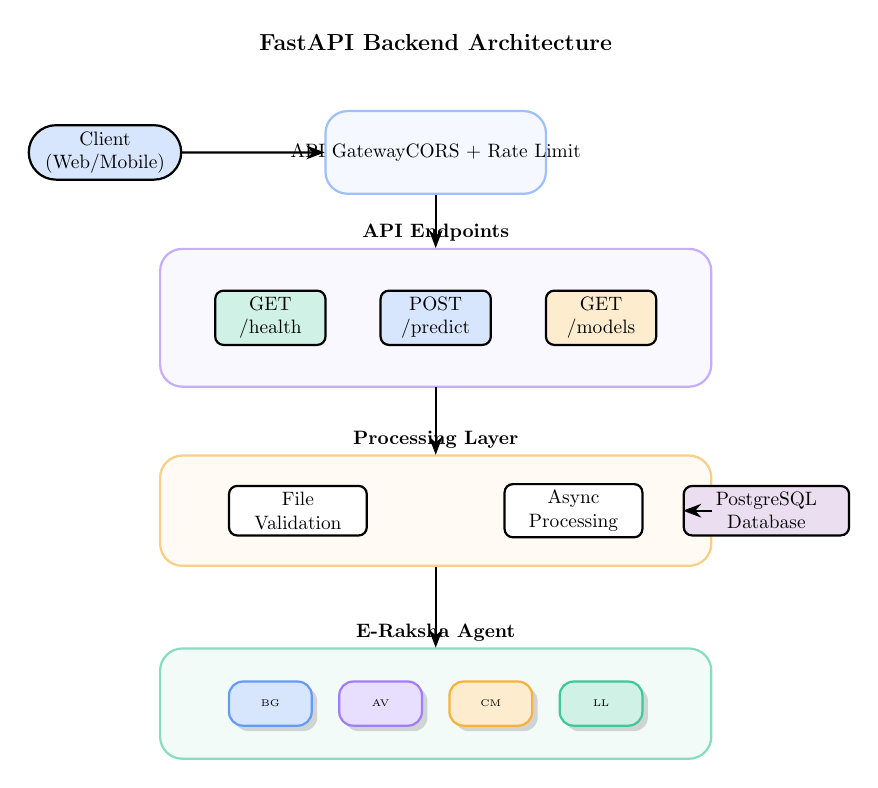
\begin{tikzpicture}[scale=0.7, transform shape]
    
    % Title
    \node[font=\large\bfseries] at (0,9) {FastAPI Backend Architecture};
    
    % Client
    \node[startstop, minimum width=3cm] (client) at (-6,7) {Client\\(Web/Mobile)};
    
    % API Gateway
    \begin{scope}[shift={(0,7)}]
        \node[container=erakshaPrimary, minimum width=4cm, minimum height=1.5cm] (gateway) {};
        \node at (gateway) {API Gateway\\CORS + Rate Limit};
    \end{scope}
    
    % Endpoints
    \begin{scope}[shift={(0,4)}]
        \node[container=erakshaSecondary, minimum width=10cm, minimum height=2.5cm] (endpoints) {};
        \node[above, font=\bfseries] at (endpoints.north) {API Endpoints};
        
        \node[process, fill=erakshaAccent!20, minimum width=2cm] at (-3,0) {GET\\/health};
        \node[process, fill=erakshaPrimary!20, minimum width=2cm] at (0,0) {POST\\/predict};
        \node[process, fill=erakshaWarning!20, minimum width=2cm] at (3,0) {GET\\/models};
    \end{scope}
    
    % Processing Layer
    \begin{scope}[shift={(0,0.5)}]
        \node[container=erakshaWarning, minimum width=10cm, minimum height=2cm] (processing) {};
        \node[above, font=\bfseries] at (processing.north) {Processing Layer};
        
        \node[process, minimum width=2.5cm] at (-2.5,0) {File\\Validation};
        \node[process, minimum width=2.5cm] at (2.5,0) {Async\\Processing};
    \end{scope}
    
    % Agent
    \begin{scope}[shift={(0,-3)}]
        \node[container=erakshaAccent, minimum width=10cm, minimum height=2cm] (agent) {};
        \node[above, font=\bfseries] at (agent.north) {E-Raksha Agent};
        
        \node[bgmodel, minimum width=1.5cm, minimum height=0.8cm, font=\tiny] at (-3,0) {BG};
        \node[avmodel, minimum width=1.5cm, minimum height=0.8cm, font=\tiny] at (-1,0) {AV};
        \node[cmmodel, minimum width=1.5cm, minimum height=0.8cm, font=\tiny] at (1,0) {CM};
        \node[llmodel, minimum width=1.5cm, minimum height=0.8cm, font=\tiny] at (3,0) {LL};
    \end{scope}
    
    % Database
    \node[process, fill=fcColor!20, minimum width=3cm] (db) at (6,0.5) {PostgreSQL\\Database};
    
    % Arrows
    \draw[arrow] (client) -- (gateway);
    \draw[arrow] (gateway) -- (endpoints);
    \draw[arrow] (endpoints) -- (processing);
    \draw[arrow] (processing) -- (agent);
    \draw[arrow] (processing) -- (db);
    
\end{tikzpicture}
\caption{FastAPI Backend Architecture}
\label{fig:backend}
\end{figure}

\subsection{API Request/Response Flow}

\begin{figure}[H]
\centering
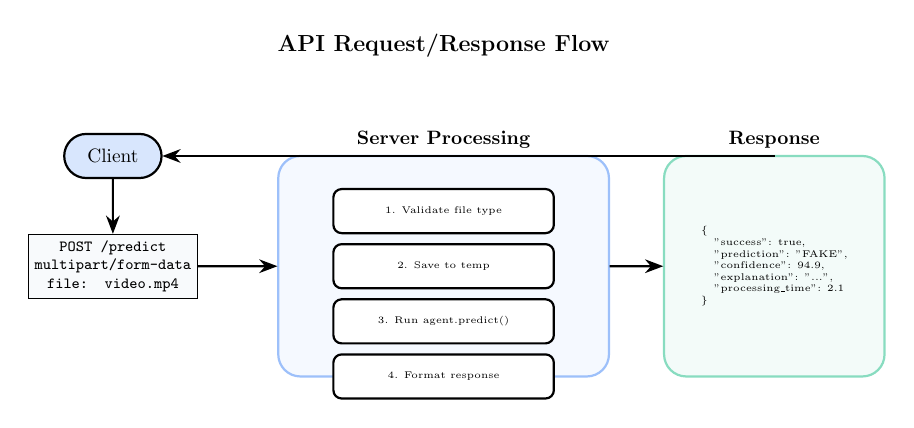
\begin{tikzpicture}[scale=0.7, transform shape]
    
    % Title
    \node[font=\large\bfseries] at (0,8) {API Request/Response Flow};
    
    % Client
    \node[startstop] (client) at (-6,6) {Client};
    
    % Request
    \node[tensor, minimum width=3cm] (request) at (-6,4) {POST /predict\\multipart/form-data\\file: video.mp4};
    
    % Server processing
    \begin{scope}[shift={(0,4)}]
        \node[container=erakshaPrimary, minimum width=6cm, minimum height=4cm] (server) {};
        \node[above, font=\bfseries] at (server.north) {Server Processing};
        
        \node[process, minimum width=4cm, font=\tiny] at (0,1) {1. Validate file type};
        \node[process, minimum width=4cm, font=\tiny] at (0,0) {2. Save to temp};
        \node[process, minimum width=4cm, font=\tiny] at (0,-1) {3. Run agent.predict()};
        \node[process, minimum width=4cm, font=\tiny] at (0,-2) {4. Format response};
    \end{scope}
    
    % Response
    \begin{scope}[shift={(6,4)}]
        \node[container=erakshaAccent, minimum width=4cm, minimum height=4cm] (response) {};
        \node[above, font=\bfseries] at (response.north) {Response};
        
        \node[font=\tiny, align=left] at (0,0) {
            \texttt{\{}\\
            \quad "success": true,\\
            \quad "prediction": "FAKE",\\
            \quad "confidence": 94.9,\\
            \quad "explanation": "...",\\
            \quad "processing\_time": 2.1\\
            \texttt{\}}
        };
    \end{scope}
    
    % Arrows
    \draw[arrow] (client) -- (request);
    \draw[arrow] (request) -- (server);
    \draw[arrow] (server) -- (response);
    \draw[arrow] (response) |- (client);
    
\end{tikzpicture}
\caption{API Request/Response Flow}
\label{fig:api-flow}
\end{figure}

\subsection{Database Schema}

\begin{figure}[H]
\centering
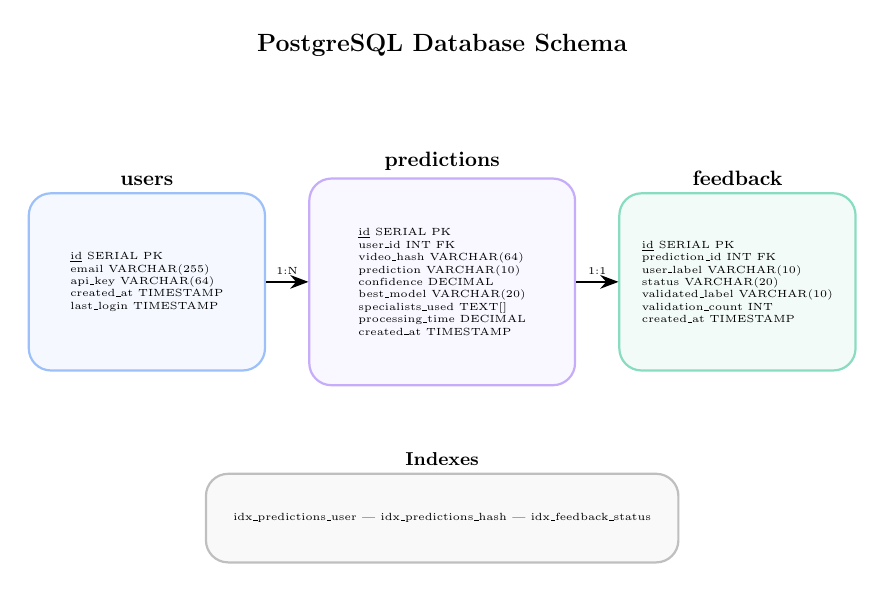
\begin{tikzpicture}[scale=0.75, transform shape]
    
    % Title
    \node[font=\large\bfseries] at (0,8) {PostgreSQL Database Schema};
    
    % Users table
    \begin{scope}[shift={(-5,4)}]
        \node[container=erakshaPrimary, minimum width=4cm, minimum height=3cm] (users) {};
        \node[above, font=\bfseries] at (users.north) {users};
        \node[font=\tiny, align=left] at (0,0) {
            \underline{id} SERIAL PK\\
            email VARCHAR(255)\\
            api\_key VARCHAR(64)\\
            created\_at TIMESTAMP\\
            last\_login TIMESTAMP
        };
    \end{scope}
    
    % Predictions table
    \begin{scope}[shift={(0,4)}]
        \node[container=erakshaSecondary, minimum width=4.5cm, minimum height=3.5cm] (predictions) {};
        \node[above, font=\bfseries] at (predictions.north) {predictions};
        \node[font=\tiny, align=left] at (0,0) {
            \underline{id} SERIAL PK\\
            user\_id INT FK\\
            video\_hash VARCHAR(64)\\
            prediction VARCHAR(10)\\
            confidence DECIMAL\\
            best\_model VARCHAR(20)\\
            specialists\_used TEXT[]\\
            processing\_time DECIMAL\\
            created\_at TIMESTAMP
        };
    \end{scope}
    
    % Feedback table
    \begin{scope}[shift={(5,4)}]
        \node[container=erakshaAccent, minimum width=4cm, minimum height=3cm] (feedback) {};
        \node[above, font=\bfseries] at (feedback.north) {feedback};
        \node[font=\tiny, align=left] at (0,0) {
            \underline{id} SERIAL PK\\
            prediction\_id INT FK\\
            user\_label VARCHAR(10)\\
            status VARCHAR(20)\\
            validated\_label VARCHAR(10)\\
            validation\_count INT\\
            created\_at TIMESTAMP
        };
    \end{scope}
    
    % Relationships
    \draw[arrow, thick] (users.east) -- node[above, font=\tiny] {1:N} (predictions.west);
    \draw[arrow, thick] (predictions.east) -- node[above, font=\tiny] {1:1} (feedback.west);
    
    % Indexes
    \begin{scope}[shift={(0,0)}]
        \node[container=gray, minimum width=8cm, minimum height=1.5cm] (indexes) {};
        \node[above, font=\bfseries\small] at (indexes.north) {Indexes};
        \node[font=\tiny] at (0,0) {
            idx\_predictions\_user | idx\_predictions\_hash | idx\_feedback\_status
        };
    \end{scope}
    
\end{tikzpicture}
\caption{PostgreSQL Database Schema}
\label{fig:database}
\end{figure}

\newpage

%%%%%%%%%%%%%%%%%%%%%%%%%%%%%%%%%%%%%%%%%%%%%%%%%%%%%%%%%%%%%%%%%%%%%%%%%%%%%%%
%% SECTION 9: DEPLOYMENT ARCHITECTURE
%%%%%%%%%%%%%%%%%%%%%%%%%%%%%%%%%%%%%%%%%%%%%%%%%%%%%%%%%%%%%%%%%%%%%%%%%%%%%%%
\section{Deployment Architecture}

\subsection{Multi-Platform Deployment}

\begin{figure}[H]
\centering
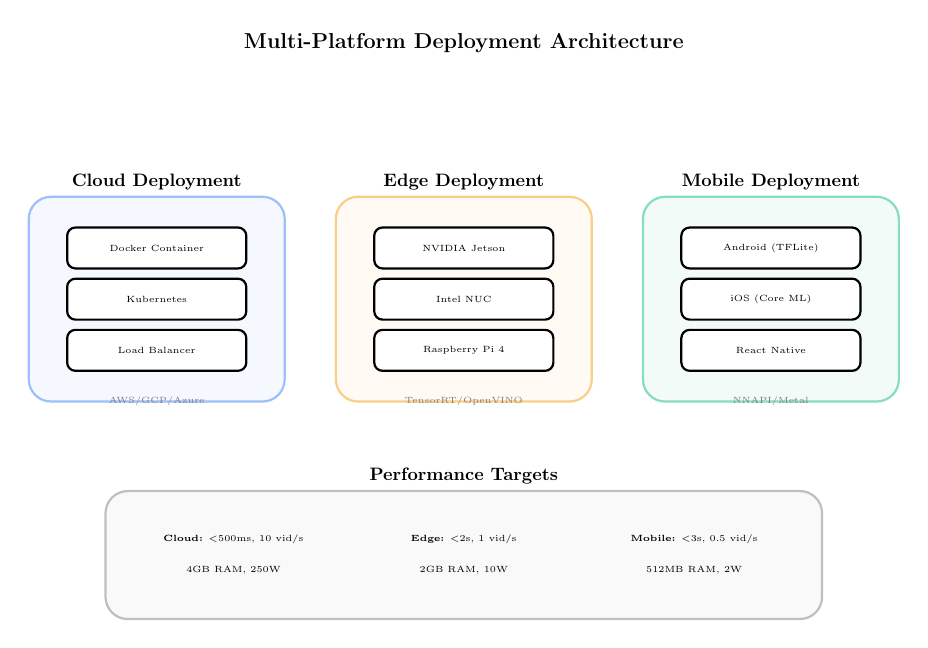
\begin{tikzpicture}[scale=0.65, transform shape]
    
    % Title
    \node[font=\large\bfseries] at (0,10) {Multi-Platform Deployment Architecture};
    
    % Cloud
    \begin{scope}[shift={(-6,5)}]
        \node[container=erakshaPrimary, minimum width=5cm, minimum height=4cm] (cloud) {};
        \node[above, font=\bfseries] at (cloud.north) {Cloud Deployment};
        
        \node[process, minimum width=3.5cm, font=\tiny] at (0,1) {Docker Container};
        \node[process, minimum width=3.5cm, font=\tiny] at (0,0) {Kubernetes};
        \node[process, minimum width=3.5cm, font=\tiny] at (0,-1) {Load Balancer};
        
        \node[font=\tiny, text=gray] at (0,-2) {AWS/GCP/Azure};
    \end{scope}
    
    % Edge
    \begin{scope}[shift={(0,5)}]
        \node[container=erakshaWarning, minimum width=5cm, minimum height=4cm] (edge) {};
        \node[above, font=\bfseries] at (edge.north) {Edge Deployment};
        
        \node[process, minimum width=3.5cm, font=\tiny] at (0,1) {NVIDIA Jetson};
        \node[process, minimum width=3.5cm, font=\tiny] at (0,0) {Intel NUC};
        \node[process, minimum width=3.5cm, font=\tiny] at (0,-1) {Raspberry Pi 4};
        
        \node[font=\tiny, text=gray] at (0,-2) {TensorRT/OpenVINO};
    \end{scope}
    
    % Mobile
    \begin{scope}[shift={(6,5)}]
        \node[container=erakshaAccent, minimum width=5cm, minimum height=4cm] (mobile) {};
        \node[above, font=\bfseries] at (mobile.north) {Mobile Deployment};
        
        \node[process, minimum width=3.5cm, font=\tiny] at (0,1) {Android (TFLite)};
        \node[process, minimum width=3.5cm, font=\tiny] at (0,0) {iOS (Core ML)};
        \node[process, minimum width=3.5cm, font=\tiny] at (0,-1) {React Native};
        
        \node[font=\tiny, text=gray] at (0,-2) {NNAPI/Metal};
    \end{scope}
    
    % Performance targets
    \begin{scope}[shift={(0,0)}]
        \node[container=gray, minimum width=14cm, minimum height=2.5cm] (perf) {};
        \node[above, font=\bfseries] at (perf.north) {Performance Targets};
        
        \node[font=\tiny] at (-4.5,0.3) {\textbf{Cloud:} $<$500ms, 10 vid/s};
        \node[font=\tiny] at (-4.5,-0.3) {4GB RAM, 250W};
        
        \node[font=\tiny] at (0,0.3) {\textbf{Edge:} $<$2s, 1 vid/s};
        \node[font=\tiny] at (0,-0.3) {2GB RAM, 10W};
        
        \node[font=\tiny] at (4.5,0.3) {\textbf{Mobile:} $<$3s, 0.5 vid/s};
        \node[font=\tiny] at (4.5,-0.3) {512MB RAM, 2W};
    \end{scope}
    
\end{tikzpicture}
\caption{Multi-Platform Deployment Architecture}
\label{fig:deployment}
\end{figure}

\subsection{Docker Deployment Stack}

\begin{figure}[H]
\centering
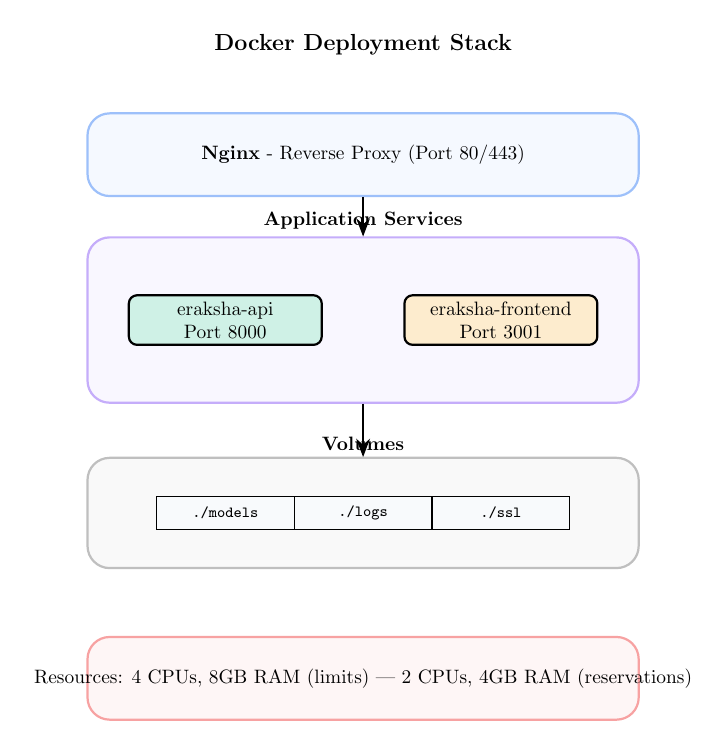
\begin{tikzpicture}[scale=0.7, transform shape]
    
    % Title
    \node[font=\large\bfseries] at (0,8) {Docker Deployment Stack};
    
    % Nginx
    \begin{scope}[shift={(0,6)}]
        \node[container=erakshaPrimary, minimum width=10cm, minimum height=1.5cm] (nginx) {};
        \node at (nginx) {\textbf{Nginx} - Reverse Proxy (Port 80/443)};
    \end{scope}
    
    % Services
    \begin{scope}[shift={(0,3)}]
        \node[container=erakshaSecondary, minimum width=10cm, minimum height=3cm] (services) {};
        \node[above, font=\bfseries] at (services.north) {Application Services};
        
        \node[process, fill=erakshaAccent!20, minimum width=3.5cm] at (-2.5,0) {eraksha-api\\Port 8000};
        \node[process, fill=erakshaWarning!20, minimum width=3.5cm] at (2.5,0) {eraksha-frontend\\Port 3001};
    \end{scope}
    
    % Volumes
    \begin{scope}[shift={(0,-0.5)}]
        \node[container=gray, minimum width=10cm, minimum height=2cm] (volumes) {};
        \node[above, font=\bfseries] at (volumes.north) {Volumes};
        
        \node[tensor, minimum width=2.5cm] at (-2.5,0) {./models};
        \node[tensor, minimum width=2.5cm] at (0,0) {./logs};
        \node[tensor, minimum width=2.5cm] at (2.5,0) {./ssl};
    \end{scope}
    
    % Resources
    \begin{scope}[shift={(0,-3.5)}]
        \node[container=erakshaDanger, minimum width=10cm, minimum height=1.5cm] (resources) {};
        \node at (resources) {Resources: 4 CPUs, 8GB RAM (limits) | 2 CPUs, 4GB RAM (reservations)};
    \end{scope}
    
    % Arrows
    \draw[arrow] (nginx) -- (services);
    \draw[arrow] (services) -- (volumes);
    
\end{tikzpicture}
\caption{Docker Compose Deployment Stack}
\label{fig:docker}
\end{figure}

\subsection{Kubernetes Deployment}

\begin{figure}[H]
\centering
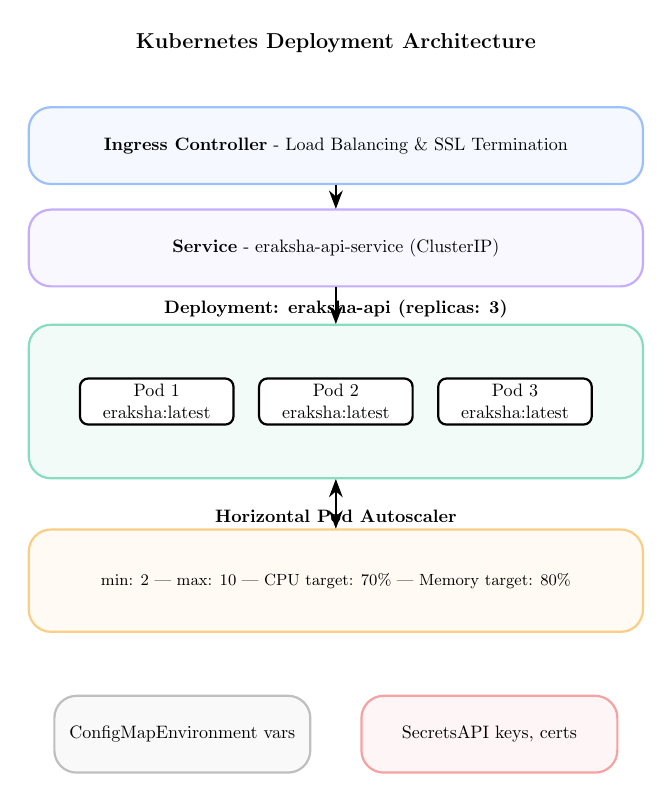
\begin{tikzpicture}[scale=0.65, transform shape]
    
    % Title
    \node[font=\large\bfseries] at (0,9) {Kubernetes Deployment Architecture};
    
    % Ingress
    \node[container=erakshaPrimary, minimum width=12cm, minimum height=1.5cm] (ingress) at (0,7) {};
    \node at (ingress) {\textbf{Ingress Controller} - Load Balancing \& SSL Termination};
    
    % Service
    \node[container=erakshaSecondary, minimum width=12cm, minimum height=1.5cm] (service) at (0,5) {};
    \node at (service) {\textbf{Service} - eraksha-api-service (ClusterIP)};
    
    % Deployment
    \begin{scope}[shift={(0,2)}]
        \node[container=erakshaAccent, minimum width=12cm, minimum height=3cm] (deployment) {};
        \node[above, font=\bfseries] at (deployment.north) {Deployment: eraksha-api (replicas: 3)};
        
        \node[process, fill=white, minimum width=3cm] at (-3.5,0) {Pod 1\\eraksha:latest};
        \node[process, fill=white, minimum width=3cm] at (0,0) {Pod 2\\eraksha:latest};
        \node[process, fill=white, minimum width=3cm] at (3.5,0) {Pod 3\\eraksha:latest};
    \end{scope}
    
    % HPA
    \begin{scope}[shift={(0,-1.5)}]
        \node[container=erakshaWarning, minimum width=12cm, minimum height=2cm] (hpa) {};
        \node[above, font=\bfseries] at (hpa.north) {Horizontal Pod Autoscaler};
        
        \node[font=\small] at (0,0) {min: 2 | max: 10 | CPU target: 70\% | Memory target: 80\%};
    \end{scope}
    
    % ConfigMap & Secrets
    \begin{scope}[shift={(0,-4.5)}]
        \node[container=gray, minimum width=5cm, minimum height=1.5cm] at (-3,0) {};
        \node at (-3,0) {ConfigMap\\Environment vars};
        
        \node[container=erakshaDanger, minimum width=5cm, minimum height=1.5cm] at (3,0) {};
        \node at (3,0) {Secrets\\API keys, certs};
    \end{scope}
    
    % Arrows
    \draw[arrow] (ingress) -- (service);
    \draw[arrow] (service) -- (deployment);
    \draw[doublearrow] (hpa) -- (deployment);
    
\end{tikzpicture}
\caption{Kubernetes Deployment with HPA}
\label{fig:kubernetes}
\end{figure}

\subsection{Model Optimization Pipeline}

\begin{figure}[H]
\centering
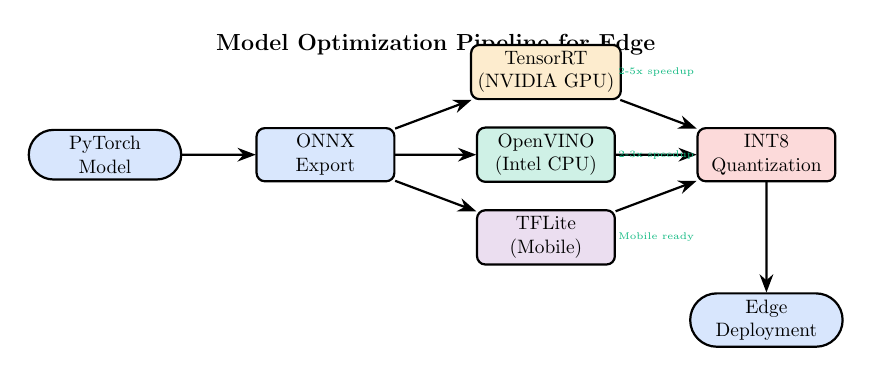
\begin{tikzpicture}[scale=0.7, transform shape]
    
    % Title
    \node[font=\large\bfseries] at (0,7) {Model Optimization Pipeline for Edge};
    
    % PyTorch Model
    \node[startstop, minimum width=3cm] (pytorch) at (-6,5) {PyTorch\\Model};
    
    % ONNX Export
    \node[process, fill=convColor!20] (onnx) at (-2,5) {ONNX\\Export};
    
    % Optimization branches
    \node[process, fill=erakshaWarning!20] (tensorrt) at (2,6.5) {TensorRT\\(NVIDIA GPU)};
    \node[process, fill=erakshaAccent!20] (openvino) at (2,5) {OpenVINO\\(Intel CPU)};
    \node[process, fill=fcColor!20] (tflite) at (2,3.5) {TFLite\\(Mobile)};
    
    % Quantization
    \node[process, fill=erakshaDanger!20] (quant) at (6,5) {INT8\\Quantization};
    
    % Deployment
    \node[startstop, minimum width=3cm] (deploy) at (6,2) {Edge\\Deployment};
    
    % Arrows
    \draw[arrow] (pytorch) -- (onnx);
    \draw[arrow] (onnx) -- (tensorrt);
    \draw[arrow] (onnx) -- (openvino);
    \draw[arrow] (onnx) -- (tflite);
    \draw[arrow] (tensorrt) -- (quant);
    \draw[arrow] (openvino) -- (quant);
    \draw[arrow] (tflite) -- (quant);
    \draw[arrow] (quant) -- (deploy);
    
    % Speedup annotations
    \node[font=\tiny, text=erakshaAccent] at (4,6.5) {2-5x speedup};
    \node[font=\tiny, text=erakshaAccent] at (4,5) {2-3x speedup};
    \node[font=\tiny, text=erakshaAccent] at (4,3.5) {Mobile ready};
    
\end{tikzpicture}
\caption{Model Optimization Pipeline for Edge Deployment}
\label{fig:optimization}
\end{figure}

\newpage

%%%%%%%%%%%%%%%%%%%%%%%%%%%%%%%%%%%%%%%%%%%%%%%%%%%%%%%%%%%%%%%%%%%%%%%%%%%%%%%
%% SECTION 10: SAFE LEARNING AND SECURITY
%%%%%%%%%%%%%%%%%%%%%%%%%%%%%%%%%%%%%%%%%%%%%%%%%%%%%%%%%%%%%%%%%%%%%%%%%%%%%%%
\section{Safe Learning and Security}

\subsection{Safe Learning Pipeline}

\begin{figure}[H]
\centering
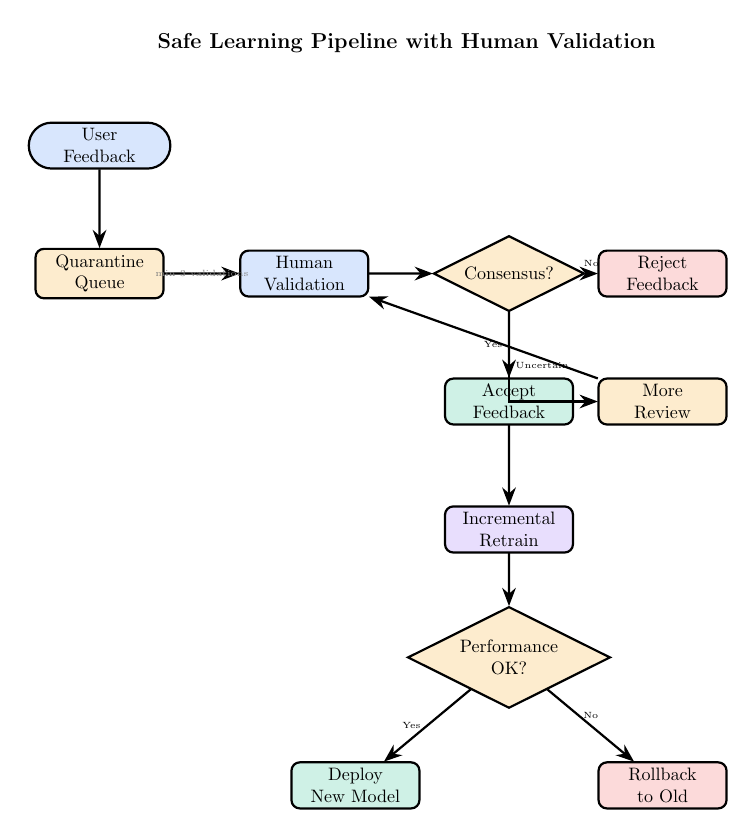
\begin{tikzpicture}[scale=0.65, transform shape]
    
    % Title
    \node[font=\large\bfseries] at (0,11) {Safe Learning Pipeline with Human Validation};
    
    % User Feedback
    \node[startstop, minimum width=3cm] (feedback) at (-6,9) {User\\Feedback};
    
    % Quarantine
    \node[process, fill=erakshaWarning!20] (quarantine) at (-6,6.5) {Quarantine\\Queue};
    
    % Human Validation
    \node[process, fill=erakshaPrimary!20] (validation) at (-2,6.5) {Human\\Validation};
    
    % Consensus Check
    \node[decision] (consensus) at (2,6.5) {Consensus?};
    
    % Accept/Reject
    \node[process, fill=erakshaAccent!20] (accept) at (2,4) {Accept\\Feedback};
    \node[process, fill=erakshaDanger!20] (reject) at (5,6.5) {Reject\\Feedback};
    \node[process, fill=erakshaWarning!20] (more) at (5,4) {More\\Review};
    
    % Incremental Retrain
    \node[process, fill=erakshaSecondary!20] (retrain) at (2,1.5) {Incremental\\Retrain};
    
    % Validate Performance
    \node[decision] (validate) at (2,-1) {Performance\\OK?};
    
    % Deploy/Rollback
    \node[process, fill=erakshaAccent!20] (deploy) at (-1,-3.5) {Deploy\\New Model};
    \node[process, fill=erakshaDanger!20] (rollback) at (5,-3.5) {Rollback\\to Old};
    
    % Arrows
    \draw[arrow] (feedback) -- (quarantine);
    \draw[arrow] (quarantine) -- (validation);
    \draw[arrow] (validation) -- (consensus);
    \draw[arrow] (consensus) -- node[left, font=\tiny] {Yes} (accept);
    \draw[arrow] (consensus) -- node[above, font=\tiny] {No} (reject);
    \draw[arrow] (consensus) |- node[right, font=\tiny, pos=0.3] {Uncertain} (more);
    \draw[arrow] (more) -- (validation);
    \draw[arrow] (accept) -- (retrain);
    \draw[arrow] (retrain) -- (validate);
    \draw[arrow] (validate) -- node[left, font=\tiny] {Yes} (deploy);
    \draw[arrow] (validate) -- node[above, font=\tiny] {No} (rollback);
    
    % Min validations annotation
    \node[font=\tiny, text=gray] at (-4,6.5) {min 3 validations};
    
\end{tikzpicture}
\caption{Safe Learning Pipeline with Human-in-the-Loop}
\label{fig:safe-learning}
\end{figure}

\subsection{Model Security Architecture}

\begin{figure}[H]
\centering
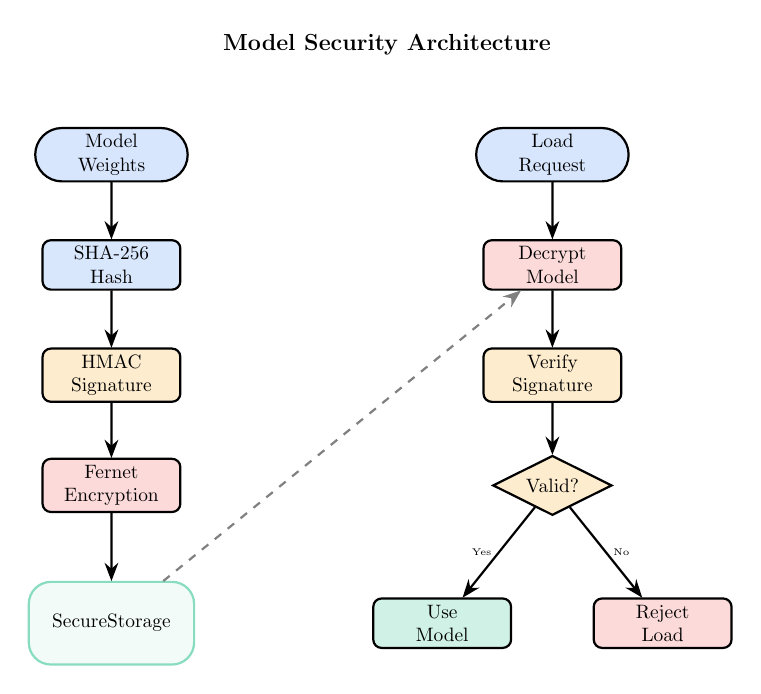
\begin{tikzpicture}[scale=0.7, transform shape]
    
    % Title
    \node[font=\large\bfseries] at (0,7) {Model Security Architecture};
    
    % Model File
    \node[startstop, minimum width=3cm] (model) at (-5,5) {Model\\Weights};
    
    % Hash
    \node[process, fill=convColor!20] (hash) at (-5,3) {SHA-256\\Hash};
    
    % Sign
    \node[process, fill=erakshaWarning!20] (sign) at (-5,1) {HMAC\\Signature};
    
    % Encrypt
    \node[process, fill=erakshaDanger!20] (encrypt) at (-5,-1) {Fernet\\Encryption};
    
    % Secure Storage
    \node[container=erakshaAccent, minimum width=3cm, minimum height=1.5cm] (storage) at (-5,-3.5) {};
    \node at (storage) {Secure\\Storage};
    
    % Verification flow
    \begin{scope}[shift={(3,0)}]
        \node[startstop, minimum width=3cm] (load) at (0,5) {Load\\Request};
        
        \node[process, fill=erakshaDanger!20] (decrypt) at (0,3) {Decrypt\\Model};
        
        \node[process, fill=erakshaWarning!20] (verify) at (0,1) {Verify\\Signature};
        
        \node[decision] (check) at (0,-1) {Valid?};
        
        \node[process, fill=erakshaAccent!20] (use) at (-2,-3.5) {Use\\Model};
        \node[process, fill=erakshaDanger!20] (reject) at (2,-3.5) {Reject\\Load};
    \end{scope}
    
    % Arrows
    \draw[arrow] (model) -- (hash);
    \draw[arrow] (hash) -- (sign);
    \draw[arrow] (sign) -- (encrypt);
    \draw[arrow] (encrypt) -- (storage);
    
    \draw[arrow] (load) -- (decrypt);
    \draw[arrow] (decrypt) -- (verify);
    \draw[arrow] (verify) -- (check);
    \draw[arrow] (check) -- node[left, font=\tiny] {Yes} (use);
    \draw[arrow] (check) -- node[right, font=\tiny] {No} (reject);
    
    \draw[dashedarrow, gray] (storage) -- (decrypt);
    
\end{tikzpicture}
\caption{Model Security with Encryption and Verification}
\label{fig:security}
\end{figure}

\subsection{Model Version Management}

\begin{figure}[H]
\centering
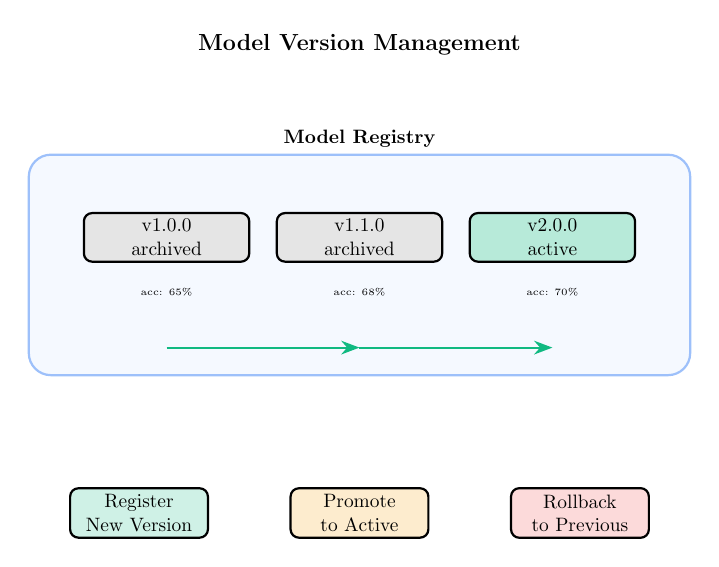
\begin{tikzpicture}[scale=0.7, transform shape]
    
    % Title
    \node[font=\large\bfseries] at (0,7) {Model Version Management};
    
    % Registry
    \begin{scope}[shift={(0,3)}]
        \node[container=erakshaPrimary, minimum width=12cm, minimum height=4cm] (registry) {};
        \node[above, font=\bfseries] at (registry.north) {Model Registry};
        
        % Versions
        \node[process, fill=gray!20, minimum width=3cm] at (-3.5,0.5) {v1.0.0\\archived};
        \node[process, fill=gray!20, minimum width=3cm] at (0,0.5) {v1.1.0\\archived};
        \node[process, fill=erakshaAccent!30, minimum width=3cm] at (3.5,0.5) {v2.0.0\\active};
        
        % Metadata
        \node[font=\tiny] at (-3.5,-0.5) {acc: 65\%};
        \node[font=\tiny] at (0,-0.5) {acc: 68\%};
        \node[font=\tiny] at (3.5,-0.5) {acc: 70\%};
    \end{scope}
    
    % Operations
    \begin{scope}[shift={(0,-1.5)}]
        \node[process, fill=erakshaAccent!20] at (-4,0) {Register\\New Version};
        \node[process, fill=erakshaWarning!20] at (0,0) {Promote\\to Active};
        \node[process, fill=erakshaDanger!20] at (4,0) {Rollback\\to Previous};
    \end{scope}
    
    % Arrows showing flow
    \draw[arrow, thick, erakshaAccent] (-3.5,1.5) -- (0,1.5);
    \draw[arrow, thick, erakshaAccent] (0,1.5) -- (3.5,1.5);
    
\end{tikzpicture}
\caption{Model Version Management with Registry}
\label{fig:versioning}
\end{figure}

\subsection{API Security}

\begin{figure}[H]
\centering
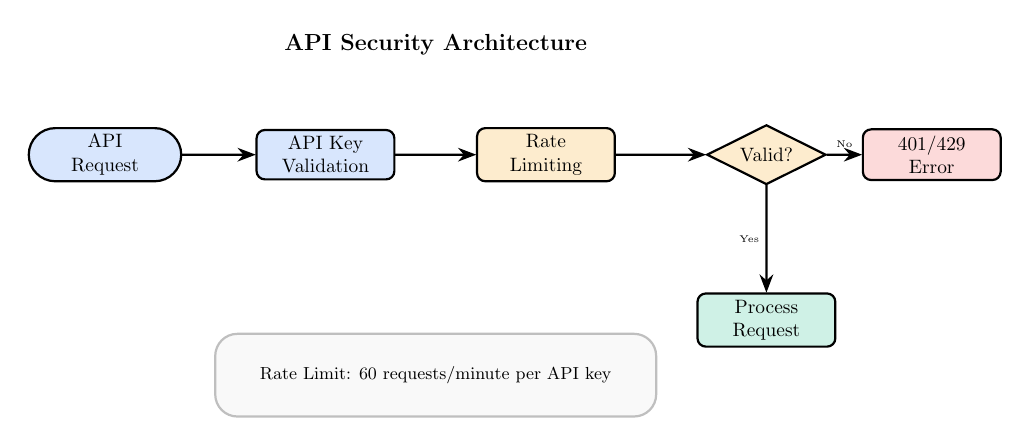
\begin{tikzpicture}[scale=0.7, transform shape]
    
    % Title
    \node[font=\large\bfseries] at (0,7) {API Security Architecture};
    
    % Request
    \node[startstop, minimum width=3cm] (request) at (-6,5) {API\\Request};
    
    % API Key Validation
    \node[process, fill=erakshaPrimary!20] (apikey) at (-2,5) {API Key\\Validation};
    
    % Rate Limiting
    \node[process, fill=erakshaWarning!20] (ratelimit) at (2,5) {Rate\\Limiting};
    
    % Decision
    \node[decision] (check) at (6,5) {Valid?};
    
    % Process or Reject
    \node[process, fill=erakshaAccent!20] (process) at (6,2) {Process\\Request};
    \node[process, fill=erakshaDanger!20] (reject) at (9,5) {401/429\\Error};
    
    % Arrows
    \draw[arrow] (request) -- (apikey);
    \draw[arrow] (apikey) -- (ratelimit);
    \draw[arrow] (ratelimit) -- (check);
    \draw[arrow] (check) -- node[left, font=\tiny] {Yes} (process);
    \draw[arrow] (check) -- node[above, font=\tiny] {No} (reject);
    
    % Rate limit details
    \begin{scope}[shift={(0,1)}]
        \node[container=gray, minimum width=8cm, minimum height=1.5cm] (details) {};
        \node[font=\small] at (0,0) {Rate Limit: 60 requests/minute per API key};
    \end{scope}
    
\end{tikzpicture}
\caption{API Security with Key Validation and Rate Limiting}
\label{fig:api-security}
\end{figure}

\newpage

%%%%%%%%%%%%%%%%%%%%%%%%%%%%%%%%%%%%%%%%%%%%%%%%%%%%%%%%%%%%%%%%%%%%%%%%%%%%%%%
%% SECTION 11: TENSOR FLOW DIAGRAMS
%%%%%%%%%%%%%%%%%%%%%%%%%%%%%%%%%%%%%%%%%%%%%%%%%%%%%%%%%%%%%%%%%%%%%%%%%%%%%%%
\section{Tensor Flow Diagrams}

\subsection{BG-Model Tensor Flow}

\begin{figure}[H]
\centering
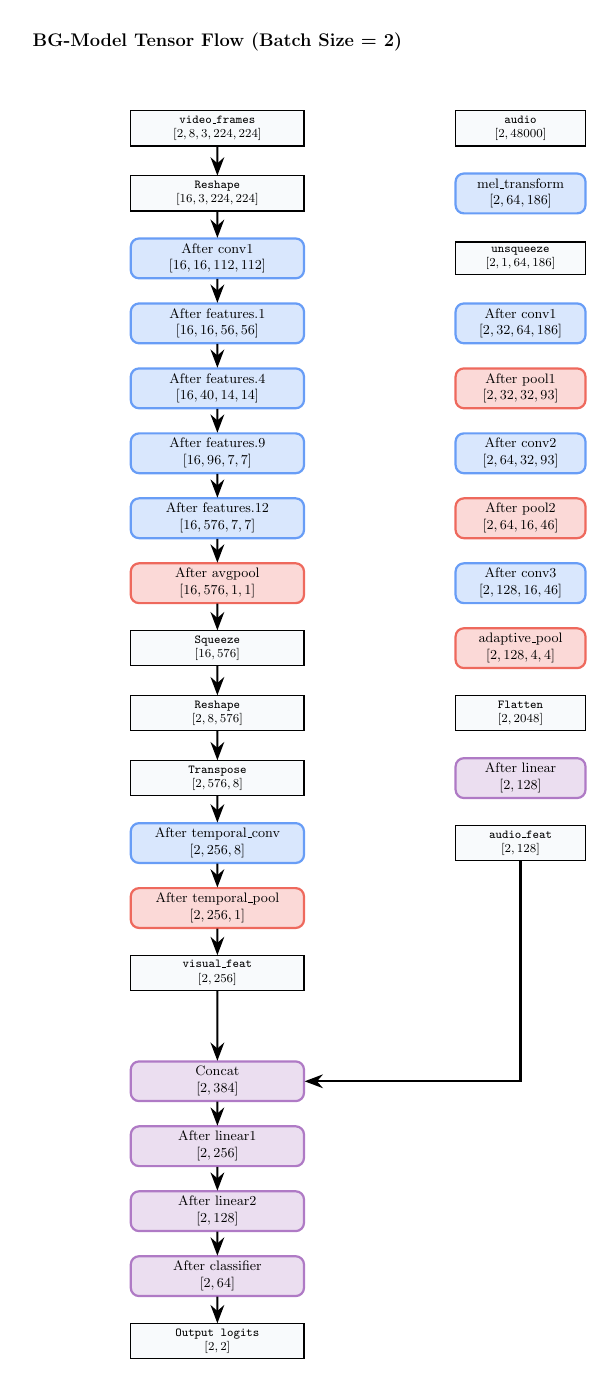
\begin{tikzpicture}[scale=0.55, transform shape, node distance=0.4cm]
    
    % Title
    \node[font=\large\bfseries] at (0,14) {BG-Model Tensor Flow (Batch Size = 2)};
    
    % Input
    \node[tensor, minimum width=4cm] (input) at (0,12) {video\_frames\\$[2, 8, 3, 224, 224]$};
    
    % Reshape for backbone
    \node[tensor, minimum width=4cm] (reshape1) at (0,10.5) {Reshape\\$[16, 3, 224, 224]$};
    
    % MobileNetV3 stages
    \node[convlayer, minimum width=4cm] (conv1) at (0,9) {After conv1\\$[16, 16, 112, 112]$};
    \node[convlayer, minimum width=4cm] (feat1) at (0,7.5) {After features.1\\$[16, 16, 56, 56]$};
    \node[convlayer, minimum width=4cm] (feat4) at (0,6) {After features.4\\$[16, 40, 14, 14]$};
    \node[convlayer, minimum width=4cm] (feat9) at (0,4.5) {After features.9\\$[16, 96, 7, 7]$};
    \node[convlayer, minimum width=4cm] (feat12) at (0,3) {After features.12\\$[16, 576, 7, 7]$};
    \node[poollayer, minimum width=4cm] (avgpool) at (0,1.5) {After avgpool\\$[16, 576, 1, 1]$};
    \node[tensor, minimum width=4cm] (squeeze) at (0,0) {Squeeze\\$[16, 576]$};
    
    % Reshape back
    \node[tensor, minimum width=4cm] (reshape2) at (0,-1.5) {Reshape\\$[2, 8, 576]$};
    
    % Temporal
    \node[tensor, minimum width=4cm] (transpose) at (0,-3) {Transpose\\$[2, 576, 8]$};
    \node[convlayer, minimum width=4cm] (tempconv) at (0,-4.5) {After temporal\_conv\\$[2, 256, 8]$};
    \node[poollayer, minimum width=4cm] (temppool) at (0,-6) {After temporal\_pool\\$[2, 256, 1]$};
    \node[tensor, minimum width=4cm] (visualfeat) at (0,-7.5) {visual\_feat\\$[2, 256]$};
    
    % Audio branch (side)
    \begin{scope}[shift={(7,6)}]
        \node[tensor, minimum width=3cm] (audio) at (0,6) {audio\\$[2, 48000]$};
        \node[convlayer, minimum width=3cm] (mel) at (0,4.5) {mel\_transform\\$[2, 64, 186]$};
        \node[tensor, minimum width=3cm] (unsqueeze) at (0,3) {unsqueeze\\$[2, 1, 64, 186]$};
        \node[convlayer, minimum width=3cm] (audconv1) at (0,1.5) {After conv1\\$[2, 32, 64, 186]$};
        \node[poollayer, minimum width=3cm] (audpool1) at (0,0) {After pool1\\$[2, 32, 32, 93]$};
        \node[convlayer, minimum width=3cm] (audconv2) at (0,-1.5) {After conv2\\$[2, 64, 32, 93]$};
        \node[poollayer, minimum width=3cm] (audpool2) at (0,-3) {After pool2\\$[2, 64, 16, 46]$};
        \node[convlayer, minimum width=3cm] (audconv3) at (0,-4.5) {After conv3\\$[2, 128, 16, 46]$};
        \node[poollayer, minimum width=3cm] (audadapt) at (0,-6) {adaptive\_pool\\$[2, 128, 4, 4]$};
        \node[tensor, minimum width=3cm] (flatten) at (0,-7.5) {Flatten\\$[2, 2048]$};
        \node[fclayer, minimum width=3cm] (audfc) at (0,-9) {After linear\\$[2, 128]$};
        \node[tensor, minimum width=3cm] (audiofeat) at (0,-10.5) {audio\_feat\\$[2, 128]$};
    \end{scope}
    
    % Fusion
    \begin{scope}[shift={(0,-10)}]
        \node[fclayer, minimum width=4cm] (concat) at (0,0) {Concat\\$[2, 384]$};
        \node[fclayer, minimum width=4cm] (fc1) at (0,-1.5) {After linear1\\$[2, 256]$};
        \node[fclayer, minimum width=4cm] (fc2) at (0,-3) {After linear2\\$[2, 128]$};
        \node[fclayer, minimum width=4cm] (fc3) at (0,-4.5) {After classifier\\$[2, 64]$};
        \node[tensor, minimum width=4cm] (output) at (0,-6) {Output logits\\$[2, 2]$};
    \end{scope}
    
    % Arrows
    \draw[arrow] (input) -- (reshape1);
    \draw[arrow] (reshape1) -- (conv1);
    \draw[arrow] (conv1) -- (feat1);
    \draw[arrow] (feat1) -- (feat4);
    \draw[arrow] (feat4) -- (feat9);
    \draw[arrow] (feat9) -- (feat12);
    \draw[arrow] (feat12) -- (avgpool);
    \draw[arrow] (avgpool) -- (squeeze);
    \draw[arrow] (squeeze) -- (reshape2);
    \draw[arrow] (reshape2) -- (transpose);
    \draw[arrow] (transpose) -- (tempconv);
    \draw[arrow] (tempconv) -- (temppool);
    \draw[arrow] (temppool) -- (visualfeat);
    
    \draw[arrow] (visualfeat) -- (concat);
    \draw[arrow] (audiofeat) |- (concat);
    \draw[arrow] (concat) -- (fc1);
    \draw[arrow] (fc1) -- (fc2);
    \draw[arrow] (fc2) -- (fc3);
    \draw[arrow] (fc3) -- (output);
    
\end{tikzpicture}
\caption{Complete Tensor Flow Through BG-Model}
\label{fig:tensor-flow-bg}
\end{figure}

\newpage

\subsection{TM-Model Tensor Flow}

\begin{figure}[H]
\centering
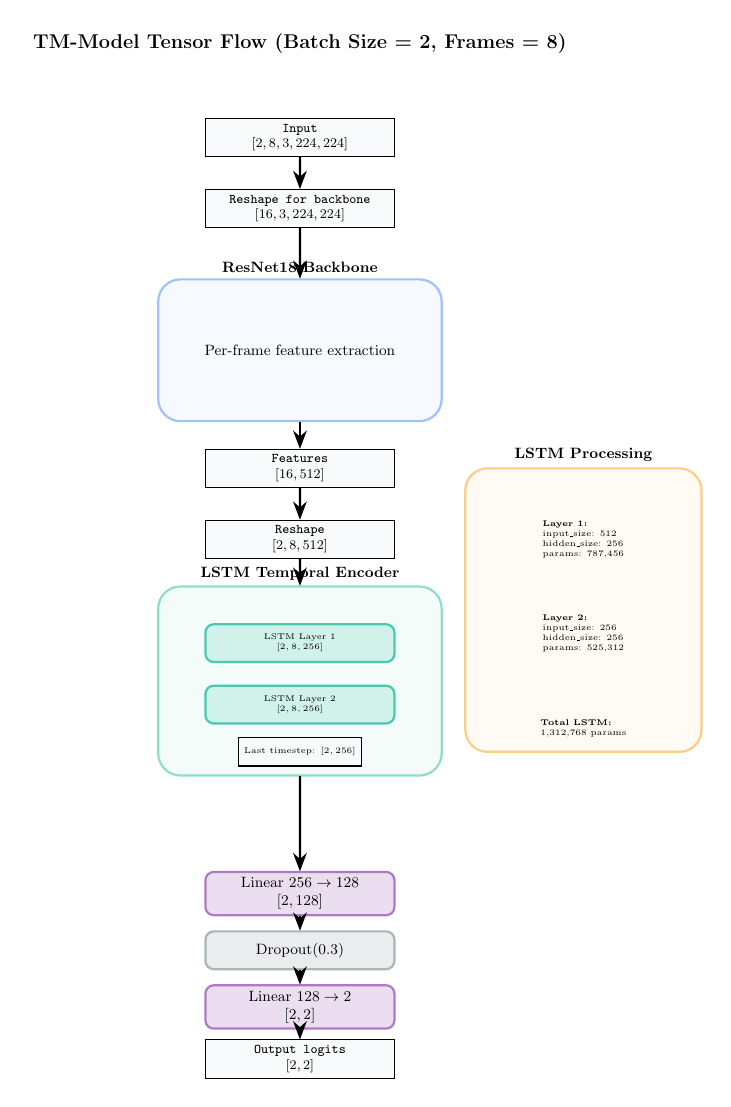
\begin{tikzpicture}[scale=0.6, transform shape, node distance=0.5cm]
    
    % Title
    \node[font=\large\bfseries] at (0,12) {TM-Model Tensor Flow (Batch Size = 2, Frames = 8)};
    
    % Input
    \node[tensor, minimum width=4cm] (input) at (0,10) {Input\\$[2, 8, 3, 224, 224]$};
    
    % Reshape
    \node[tensor, minimum width=4cm] (reshape1) at (0,8.5) {Reshape for backbone\\$[16, 3, 224, 224]$};
    
    % ResNet18
    \begin{scope}[shift={(0,5.5)}]
        \node[container=convColor, minimum width=6cm, minimum height=3cm] (resnet) {};
        \node[above, font=\bfseries\small] at (resnet.north) {ResNet18 Backbone};
        \node[font=\small] at (0,0) {Per-frame feature extraction};
    \end{scope}
    
    % Feature output
    \node[tensor, minimum width=4cm] (features) at (0,3) {Features\\$[16, 512]$};
    
    % Reshape back
    \node[tensor, minimum width=4cm] (reshape2) at (0,1.5) {Reshape\\$[2, 8, 512]$};
    
    % LSTM
    \begin{scope}[shift={(0,-1.5)}]
        \node[container=lstmColor, minimum width=6cm, minimum height=4cm] (lstm) {};
        \node[above, font=\bfseries\small] at (lstm.north) {LSTM Temporal Encoder};
        
        \node[lstmlayer, minimum width=4cm, font=\tiny] at (0,0.8) {LSTM Layer 1\\$[2, 8, 256]$};
        \node[lstmlayer, minimum width=4cm, font=\tiny] at (0,-0.5) {LSTM Layer 2\\$[2, 8, 256]$};
        \node[tensor, font=\tiny] at (0,-1.5) {Last timestep: $[2, 256]$};
    \end{scope}
    
    % Classification
    \begin{scope}[shift={(0,-6.5)}]
        \node[fclayer, minimum width=4cm] (fc1) at (0,0.5) {Linear $256 \to 128$\\$[2, 128]$};
        \node[dropoutlayer, minimum width=4cm] (drop) at (0,-0.7) {Dropout(0.3)};
        \node[fclayer, minimum width=4cm] (fc2) at (0,-1.9) {Linear $128 \to 2$\\$[2, 2]$};
    \end{scope}
    
    % Output
    \node[tensor, minimum width=4cm] (output) at (0,-9.5) {Output logits\\$[2, 2]$};
    
    % Arrows
    \draw[arrow] (input) -- (reshape1);
    \draw[arrow] (reshape1) -- (resnet);
    \draw[arrow] (resnet) -- (features);
    \draw[arrow] (features) -- (reshape2);
    \draw[arrow] (reshape2) -- (lstm);
    \draw[arrow] (lstm) -- (fc1);
    \draw[arrow] (fc1) -- (drop);
    \draw[arrow] (drop) -- (fc2);
    \draw[arrow] (fc2) -- (output);
    
    % LSTM detail
    \begin{scope}[shift={(6,0)}]
        \node[container=erakshaWarning, minimum width=5cm, minimum height=6cm] (lstmdetail) {};
        \node[above, font=\bfseries\small] at (lstmdetail.north) {LSTM Processing};
        
        \node[font=\tiny, align=left] at (0,1.5) {
            \textbf{Layer 1:}\\
            input\_size: 512\\
            hidden\_size: 256\\
            params: 787,456
        };
        
        \node[font=\tiny, align=left] at (0,-0.5) {
            \textbf{Layer 2:}\\
            input\_size: 256\\
            hidden\_size: 256\\
            params: 525,312
        };
        
        \node[font=\tiny, align=left] at (0,-2.5) {
            \textbf{Total LSTM:}\\
            1,312,768 params
        };
    \end{scope}
    
\end{tikzpicture}
\caption{Complete Tensor Flow Through TM-Model}
\label{fig:tensor-flow-tm}
\end{figure}

%%%%%%%%%%%%%%%%%%%%%%%%%%%%%%%%%%%%%%%%%%%%%%%%%%%%%%%%%%%%%%%%%%%%%%%%%%%%%%%
%% SECTION 12: MATHEMATICAL VISUALIZATIONS
%%%%%%%%%%%%%%%%%%%%%%%%%%%%%%%%%%%%%%%%%%%%%%%%%%%%%%%%%%%%%%%%%%%%%%%%%%%%%%%
\section{Mathematical Visualizations}

\subsection{Convolution Operation}

\begin{figure}[H]
\centering
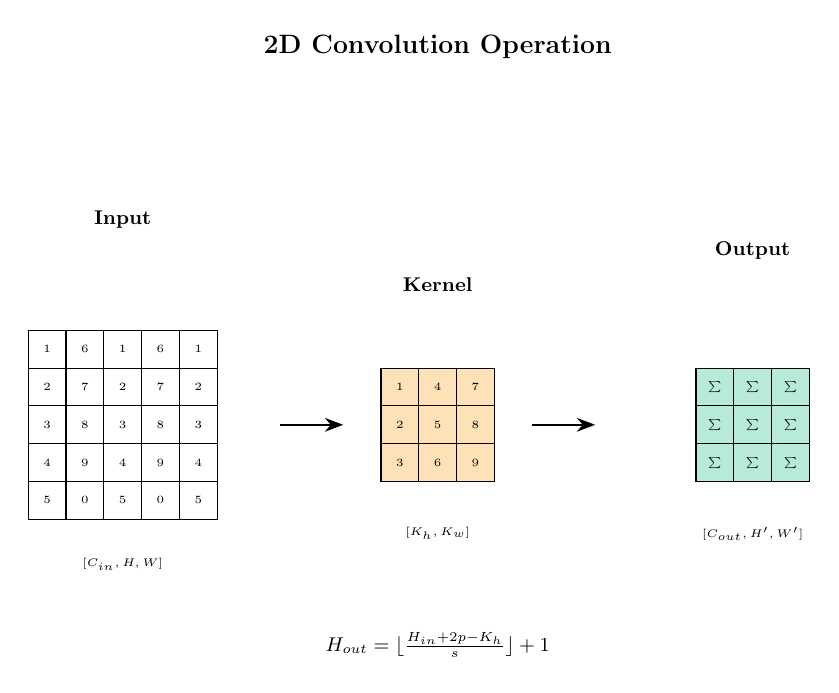
\begin{tikzpicture}[scale=0.8, transform shape]
    
    % Title
    \node[font=\large\bfseries] at (0,6) {2D Convolution Operation};
    
    % Input feature map
    \begin{scope}[shift={(-5,0)}]
        \node[above, font=\bfseries\small] at (0,3) {Input};
        \foreach \i in {0,...,4} {
            \foreach \j in {0,...,4} {
                \pgfmathsetmacro{\val}{int(mod(\i*5+\j+1,10))}
                \node[draw, minimum size=0.6cm, font=\tiny] at (\i*0.6-1.2, -\j*0.6+1.2) {\val};
            }
        }
        \node[below, font=\tiny] at (0,-2) {$[C_{in}, H, W]$};
    \end{scope}
    
    % Kernel
    \begin{scope}[shift={(0,0)}]
        \node[above, font=\bfseries\small] at (0,2) {Kernel};
        \foreach \i in {0,...,2} {
            \foreach \j in {0,...,2} {
                \pgfmathsetmacro{\val}{int(mod(\i*3+\j+1,10))}
                \node[draw, minimum size=0.6cm, fill=erakshaWarning!30, font=\tiny] at (\i*0.6-0.6, -\j*0.6+0.6) {\val};
            }
        }
        \node[below, font=\tiny] at (0,-1.5) {$[K_h, K_w]$};
    \end{scope}
    
    % Output
    \begin{scope}[shift={(5,0)}]
        \node[above, font=\bfseries\small] at (0,2.5) {Output};
        \foreach \i in {0,...,2} {
            \foreach \j in {0,...,2} {
                \node[draw, minimum size=0.6cm, fill=erakshaAccent!30, font=\tiny] at (\i*0.6-0.6, -\j*0.6+0.6) {$\sum$};
            }
        }
        \node[below, font=\tiny] at (0,-1.5) {$[C_{out}, H', W']$};
    \end{scope}
    
    % Arrows
    \draw[arrow, thick] (-2.5,0) -- (-1.5,0);
    \draw[arrow, thick] (1.5,0) -- (2.5,0);
    
    % Formula
    \node[font=\small] at (0,-3.5) {$H_{out} = \lfloor\frac{H_{in} + 2p - K_h}{s}\rfloor + 1$};
    
\end{tikzpicture}
\caption{2D Convolution Operation Visualization}
\label{fig:convolution}
\end{figure}

\subsection{Softmax and Cross-Entropy}

\begin{figure}[H]
\centering
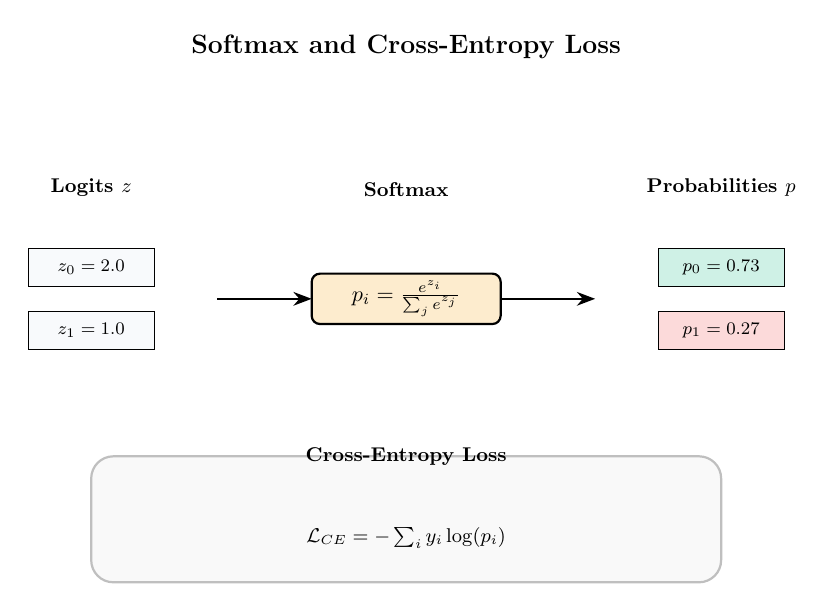
\begin{tikzpicture}[scale=0.8, transform shape]
    
    % Title
    \node[font=\large\bfseries] at (0,5) {Softmax and Cross-Entropy Loss};
    
    % Logits
    \begin{scope}[shift={(-5,0)}]
        \node[above, font=\bfseries\small] at (0,2.5) {Logits $z$};
        \node[tensor, minimum width=2cm] at (0,1.5) {$z_0 = 2.0$};
        \node[tensor, minimum width=2cm] at (0,0.5) {$z_1 = 1.0$};
    \end{scope}
    
    % Softmax
    \begin{scope}[shift={(0,0)}]
        \node[above, font=\bfseries\small] at (0,2.5) {Softmax};
        \node[process, fill=erakshaWarning!20, minimum width=3cm] at (0,1) {$p_i = \frac{e^{z_i}}{\sum_j e^{z_j}}$};
    \end{scope}
    
    % Probabilities
    \begin{scope}[shift={(5,0)}]
        \node[above, font=\bfseries\small] at (0,2.5) {Probabilities $p$};
        \node[tensor, minimum width=2cm, fill=erakshaAccent!20] at (0,1.5) {$p_0 = 0.73$};
        \node[tensor, minimum width=2cm, fill=erakshaDanger!20] at (0,0.5) {$p_1 = 0.27$};
    \end{scope}
    
    % Arrows
    \draw[arrow] (-3,1) -- (-1.5,1);
    \draw[arrow] (1.5,1) -- (3,1);
    
    % Cross-Entropy
    \node[container=gray, minimum width=10cm, minimum height=2cm] at (0,-2.5) {};
    \node[font=\bfseries\small] at (0,-1.5) {Cross-Entropy Loss};
    \node[font=\small] at (0,-2.8) {$\mathcal{L}_{CE} = -\sum_i y_i \log(p_i)$};
    
\end{tikzpicture}
\caption{Softmax and Cross-Entropy Loss Computation}
\label{fig:softmax}
\end{figure}

\newpage

\subsection{Knowledge Distillation}

\begin{figure}[H]
\centering
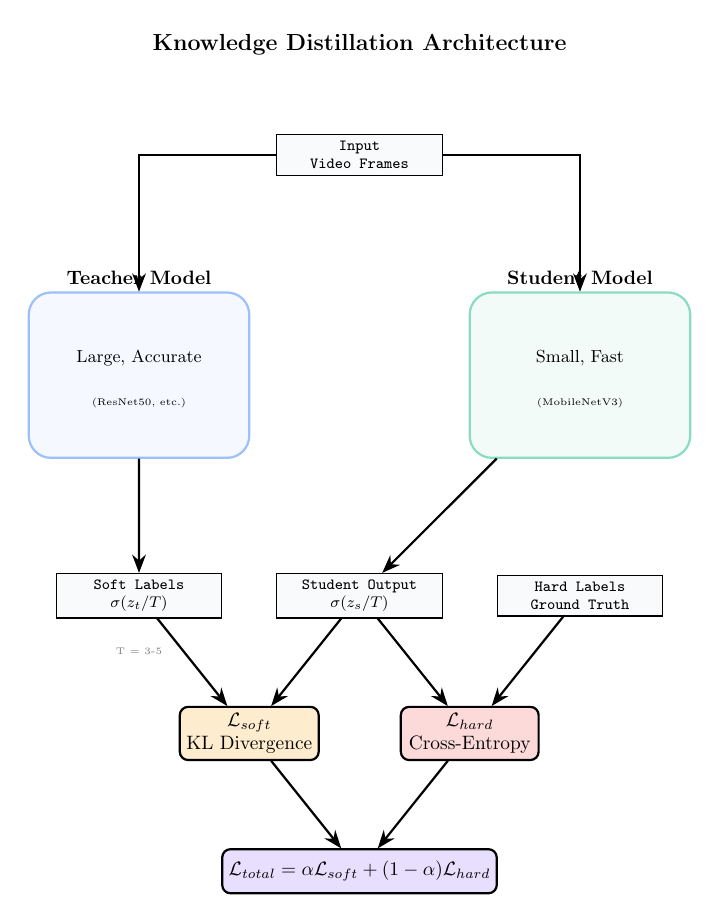
\begin{tikzpicture}[scale=0.7, transform shape]
    
    % Title
    \node[font=\large\bfseries] at (0,8) {Knowledge Distillation Architecture};
    
    % Input
    \node[tensor, minimum width=3cm] (input) at (0,6) {Input\\Video Frames};
    
    % Teacher
    \begin{scope}[shift={(-4,2)}]
        \node[container=erakshaPrimary, minimum width=4cm, minimum height=3cm] (teacher) {};
        \node[above, font=\bfseries] at (teacher.north) {Teacher Model};
        \node[font=\small] at (0,0.3) {Large, Accurate};
        \node[font=\tiny] at (0,-0.5) {(ResNet50, etc.)};
    \end{scope}
    
    % Student
    \begin{scope}[shift={(4,2)}]
        \node[container=erakshaAccent, minimum width=4cm, minimum height=3cm] (student) {};
        \node[above, font=\bfseries] at (student.north) {Student Model};
        \node[font=\small] at (0,0.3) {Small, Fast};
        \node[font=\tiny] at (0,-0.5) {(MobileNetV3)};
    \end{scope}
    
    % Soft labels
    \node[tensor, minimum width=3cm] (soft) at (-4,-2) {Soft Labels\\$\sigma(z_t/T)$};
    
    % Hard labels
    \node[tensor, minimum width=3cm] (hard) at (4,-2) {Hard Labels\\Ground Truth};
    
    % Student output
    \node[tensor, minimum width=3cm] (studentout) at (0,-2) {Student Output\\$\sigma(z_s/T)$};
    
    % Losses
    \node[process, fill=erakshaWarning!20] (softloss) at (-2,-4.5) {$\mathcal{L}_{soft}$\\KL Divergence};
    \node[process, fill=erakshaDanger!20] (hardloss) at (2,-4.5) {$\mathcal{L}_{hard}$\\Cross-Entropy};
    
    % Total loss
    \node[process, fill=erakshaSecondary!20, minimum width=4cm] (total) at (0,-7) {$\mathcal{L}_{total} = \alpha \mathcal{L}_{soft} + (1-\alpha) \mathcal{L}_{hard}$};
    
    % Arrows
    \draw[arrow] (input) -| (teacher);
    \draw[arrow] (input) -| (student);
    \draw[arrow] (teacher) -- (soft);
    \draw[arrow] (student) -- (studentout);
    \draw[arrow] (soft) -- (softloss);
    \draw[arrow] (studentout) -- (softloss);
    \draw[arrow] (studentout) -- (hardloss);
    \draw[arrow] (hard) -- (hardloss);
    \draw[arrow] (softloss) -- (total);
    \draw[arrow] (hardloss) -- (total);
    
    % Temperature annotation
    \node[font=\tiny, text=gray] at (-4,-3) {T = 3-5};
    
\end{tikzpicture}
\caption{Knowledge Distillation from Teacher to Student}
\label{fig:distillation}
\end{figure}

\subsection{Weighted Ensemble Aggregation}

\begin{figure}[H]
\centering
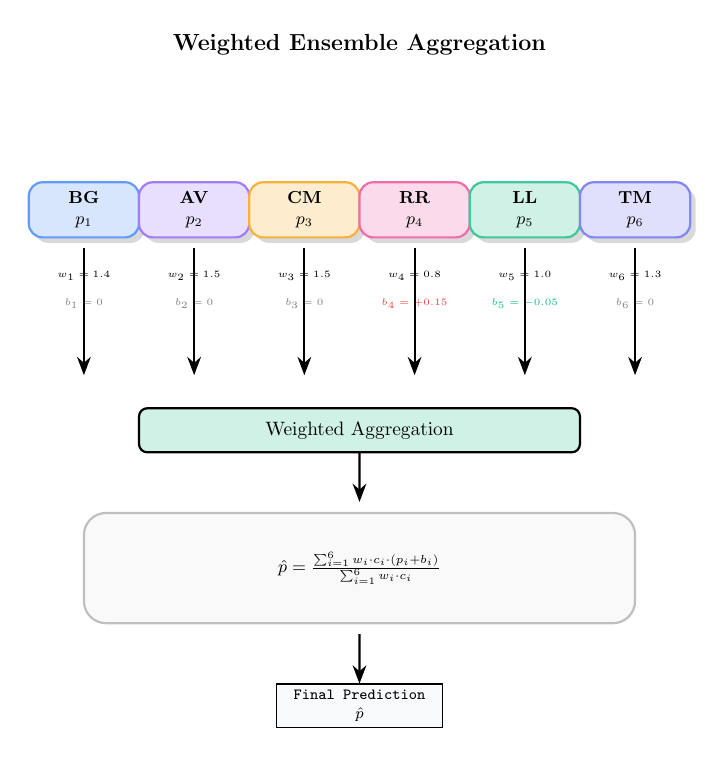
\begin{tikzpicture}[scale=0.7, transform shape]
    
    % Title
    \node[font=\large\bfseries] at (0,7) {Weighted Ensemble Aggregation};
    
    % Models
    \node[bgmodel, minimum width=2cm, minimum height=1cm] (bg) at (-5,4) {BG\\$p_1$};
    \node[avmodel, minimum width=2cm, minimum height=1cm] (av) at (-3,4) {AV\\$p_2$};
    \node[cmmodel, minimum width=2cm, minimum height=1cm] (cm) at (-1,4) {CM\\$p_3$};
    \node[rrmodel, minimum width=2cm, minimum height=1cm] (rr) at (1,4) {RR\\$p_4$};
    \node[llmodel, minimum width=2cm, minimum height=1cm] (ll) at (3,4) {LL\\$p_5$};
    \node[tmmodel, minimum width=2cm, minimum height=1cm] (tm) at (5,4) {TM\\$p_6$};
    
    % Weights
    \node[font=\tiny] at (-5,2.8) {$w_1=1.4$};
    \node[font=\tiny] at (-3,2.8) {$w_2=1.5$};
    \node[font=\tiny] at (-1,2.8) {$w_3=1.5$};
    \node[font=\tiny] at (1,2.8) {$w_4=0.8$};
    \node[font=\tiny] at (3,2.8) {$w_5=1.0$};
    \node[font=\tiny] at (5,2.8) {$w_6=1.3$};
    
    % Bias corrections
    \node[font=\tiny, text=gray] at (-5,2.3) {$b_1=0$};
    \node[font=\tiny, text=gray] at (-3,2.3) {$b_2=0$};
    \node[font=\tiny, text=gray] at (-1,2.3) {$b_3=0$};
    \node[font=\tiny, text=erakshaDanger] at (1,2.3) {$b_4=+0.15$};
    \node[font=\tiny, text=erakshaAccent] at (3,2.3) {$b_5=-0.05$};
    \node[font=\tiny, text=gray] at (5,2.3) {$b_6=0$};
    
    % Aggregation
    \node[process, fill=erakshaAccent!20, minimum width=8cm] (agg) at (0,0) {Weighted Aggregation};
    
    % Formula
    \node[container=gray, minimum width=10cm, minimum height=2cm] at (0,-2.5) {};
    \node[font=\small] at (0,-2.5) {$\hat{p} = \frac{\sum_{i=1}^{6} w_i \cdot c_i \cdot (p_i + b_i)}{\sum_{i=1}^{6} w_i \cdot c_i}$};
    
    % Output
    \node[tensor, minimum width=3cm] (output) at (0,-5) {Final Prediction\\$\hat{p}$};
    
    % Arrows
    \foreach \x in {-5,-3,-1,1,3,5} {
        \draw[arrow] (\x,3.3) -- (\x,1);
    }
    \draw[arrow] (agg) -- (0,-1.3);
    \draw[arrow] (0,-3.7) -- (output);
    
\end{tikzpicture}
\caption{Weighted Ensemble Aggregation with Bias Correction}
\label{fig:ensemble-math}
\end{figure}

\newpage

%%%%%%%%%%%%%%%%%%%%%%%%%%%%%%%%%%%%%%%%%%%%%%%%%%%%%%%%%%%%%%%%%%%%%%%%%%%%%%%
%% SECTION 13: PERFORMANCE VISUALIZATIONS
%%%%%%%%%%%%%%%%%%%%%%%%%%%%%%%%%%%%%%%%%%%%%%%%%%%%%%%%%%%%%%%%%%%%%%%%%%%%%%%
\section{Performance Visualizations}

\subsection{Model Accuracy Comparison}

\begin{figure}[H]
\centering
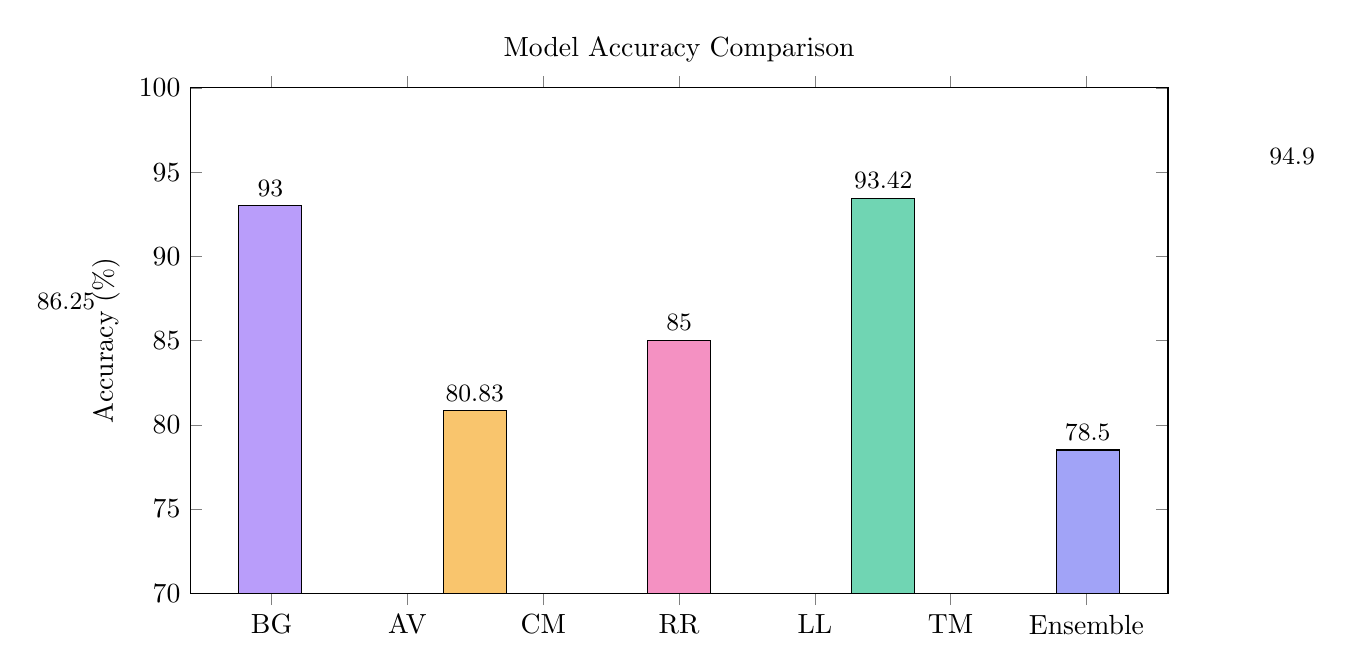
\begin{tikzpicture}
    \begin{axis}[
        ybar,
        width=14cm,
        height=8cm,
        ylabel={Accuracy (\%)},
        symbolic x coords={BG, AV, CM, RR, LL, TM, Ensemble},
        xtick=data,
        ymin=70,
        ymax=100,
        bar width=0.8cm,
        nodes near coords,
        nodes near coords align={vertical},
        every node near coord/.append style={font=\small},
        legend style={at={(0.5,-0.15)}, anchor=north, legend columns=2},
        title={Model Accuracy Comparison}
    ]
    \addplot[fill=bgModelColor!60] coordinates {(BG,86.25) (AV,0) (CM,0) (RR,0) (LL,0) (TM,0) (Ensemble,0)};
    \addplot[fill=avModelColor!60] coordinates {(BG,0) (AV,93.0) (CM,0) (RR,0) (LL,0) (TM,0) (Ensemble,0)};
    \addplot[fill=cmModelColor!60] coordinates {(BG,0) (AV,0) (CM,80.83) (RR,0) (LL,0) (TM,0) (Ensemble,0)};
    \addplot[fill=rrModelColor!60] coordinates {(BG,0) (AV,0) (CM,0) (RR,85.0) (LL,0) (TM,0) (Ensemble,0)};
    \addplot[fill=llModelColor!60] coordinates {(BG,0) (AV,0) (CM,0) (RR,0) (LL,93.42) (TM,0) (Ensemble,0)};
    \addplot[fill=tmModelColor!60] coordinates {(BG,0) (AV,0) (CM,0) (RR,0) (LL,0) (TM,78.5) (Ensemble,0)};
    \addplot[fill=erakshaAccent!60] coordinates {(BG,0) (AV,0) (CM,0) (RR,0) (LL,0) (TM,0) (Ensemble,94.9)};
    \end{axis}
\end{tikzpicture}
\caption{Individual Model and Ensemble Accuracy Comparison}
\label{fig:accuracy-chart}
\end{figure}

\subsection{Parameter Count Comparison}

\begin{figure}[H]
\centering
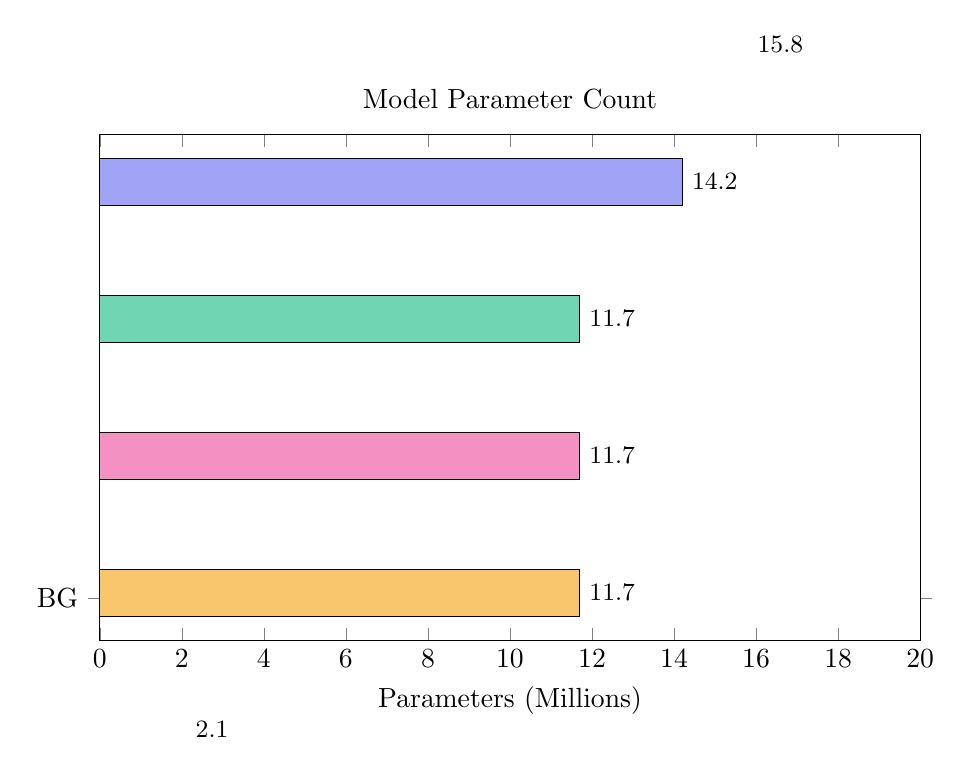
\begin{tikzpicture}
    \begin{axis}[
        xbar,
        width=12cm,
        height=8cm,
        xlabel={Parameters (Millions)},
        symbolic y coords={BG, CM, RR, LL, TM, AV},
        ytick=data,
        xmin=0,
        xmax=20,
        bar width=0.6cm,
        nodes near coords,
        nodes near coords align={horizontal},
        every node near coord/.append style={font=\small},
        title={Model Parameter Count}
    ]
    \addplot[fill=bgModelColor!60] coordinates {(2.1,BG)};
    \addplot[fill=cmModelColor!60] coordinates {(11.7,CM)};
    \addplot[fill=rrModelColor!60] coordinates {(11.7,RR)};
    \addplot[fill=llModelColor!60] coordinates {(11.7,LL)};
    \addplot[fill=tmModelColor!60] coordinates {(14.2,TM)};
    \addplot[fill=avModelColor!60] coordinates {(15.8,AV)};
    \end{axis}
\end{tikzpicture}
\caption{Model Parameter Count Comparison}
\label{fig:params-chart}
\end{figure}

\subsection{Routing Efficiency}

\begin{figure}[H]
\centering
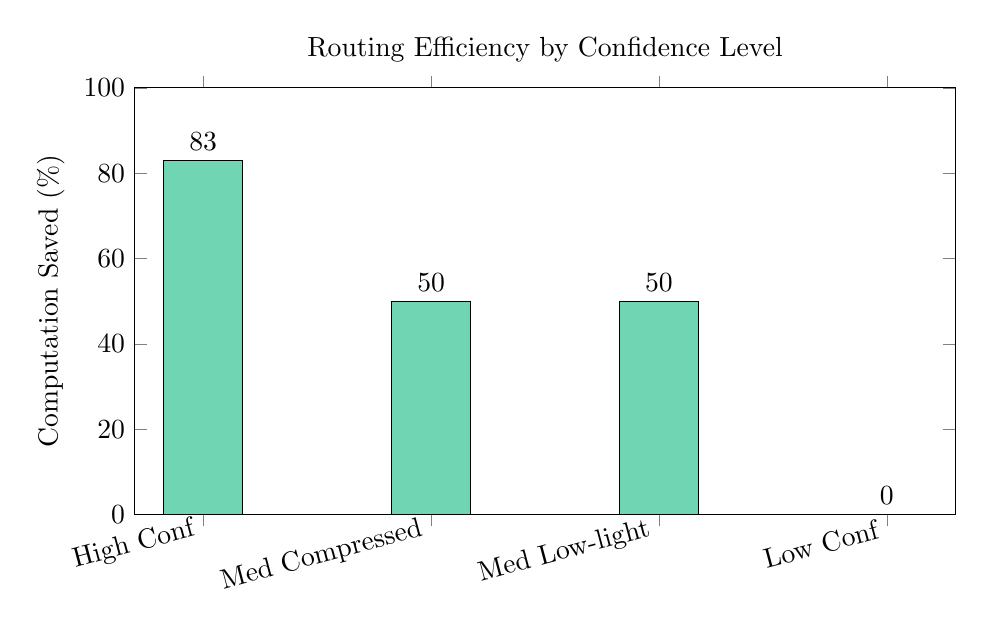
\begin{tikzpicture}
    \begin{axis}[
        ybar,
        width=12cm,
        height=7cm,
        ylabel={Computation Saved (\%)},
        symbolic x coords={High Conf, Med Compressed, Med Low-light, Low Conf},
        xtick=data,
        x tick label style={rotate=15, anchor=east},
        ymin=0,
        ymax=100,
        bar width=1cm,
        nodes near coords,
        nodes near coords align={vertical},
        title={Routing Efficiency by Confidence Level}
    ]
    \addplot[fill=erakshaAccent!60] coordinates {
        (High Conf,83)
        (Med Compressed,50)
        (Med Low-light,50)
        (Low Conf,0)
    };
    \end{axis}
\end{tikzpicture}
\caption{Computation Savings from Intelligent Routing}
\label{fig:routing-efficiency}
\end{figure}

\subsection{Bias Correction Impact}

\begin{figure}[H]
\centering
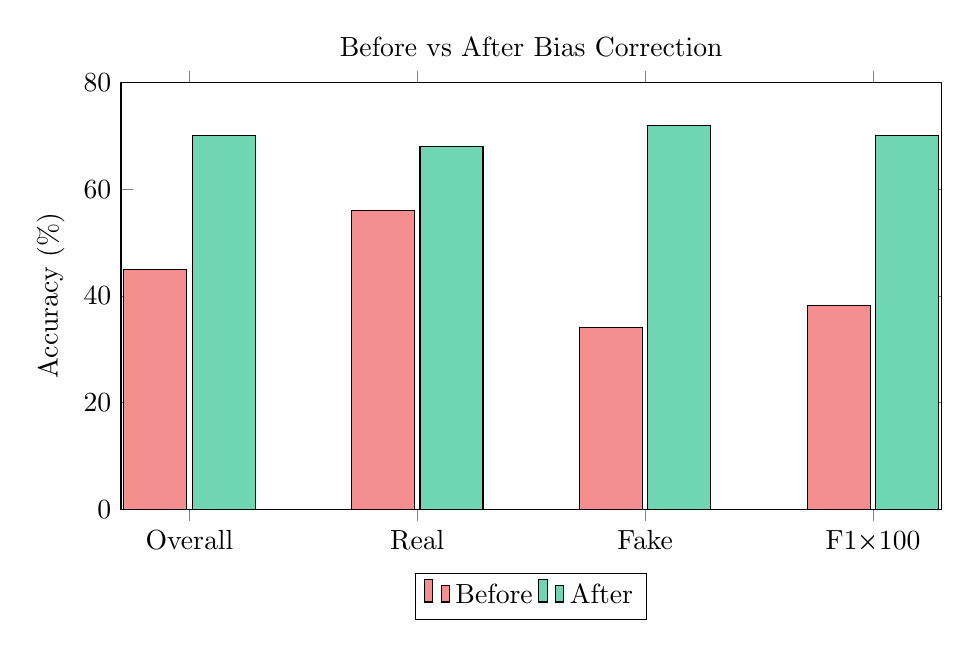
\begin{tikzpicture}
    \begin{axis}[
        ybar,
        width=12cm,
        height=7cm,
        ylabel={Accuracy (\%)},
        symbolic x coords={Overall, Real, Fake, F1×100},
        xtick=data,
        ymin=0,
        ymax=80,
        bar width=0.8cm,
        legend style={at={(0.5,-0.15)}, anchor=north, legend columns=2},
        title={Before vs After Bias Correction}
    ]
    \addplot[fill=erakshaDanger!60] coordinates {(Overall,45) (Real,56) (Fake,34) (F1×100,38.2)};
    \addplot[fill=erakshaAccent!60] coordinates {(Overall,70) (Real,68) (Fake,72) (F1×100,70)};
    \legend{Before, After}
    \end{axis}
\end{tikzpicture}
\caption{Performance Improvement from Bias Correction}
\label{fig:bias-impact}
\end{figure}

\newpage

%%%%%%%%%%%%%%%%%%%%%%%%%%%%%%%%%%%%%%%%%%%%%%%%%%%%%%%%%%%%%%%%%%%%%%%%%%%%%%%
%% SECTION 14: FRONTEND ARCHITECTURE
%%%%%%%%%%%%%%%%%%%%%%%%%%%%%%%%%%%%%%%%%%%%%%%%%%%%%%%%%%%%%%%%%%%%%%%%%%%%%%%
\section{Frontend Architecture}

\subsection{React Component Architecture}

\begin{figure}[H]
\centering
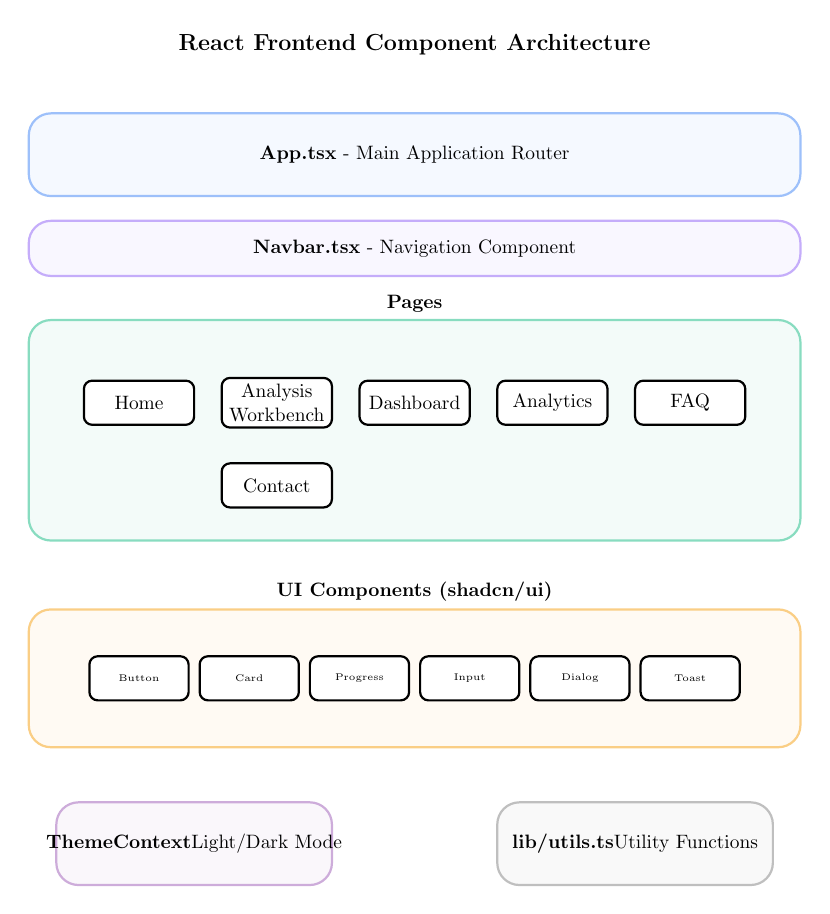
\begin{tikzpicture}[scale=0.7, transform shape]
    
    % Title
    \node[font=\large\bfseries] at (0,9) {React Frontend Component Architecture};
    
    % App
    \node[container=erakshaPrimary, minimum width=14cm, minimum height=1.5cm] (app) at (0,7) {};
    \node at (app) {\textbf{App.tsx} - Main Application Router};
    
    % Navbar
    \node[container=erakshaSecondary, minimum width=14cm, minimum height=1cm] (navbar) at (0,5.3) {};
    \node at (navbar) {\textbf{Navbar.tsx} - Navigation Component};
    
    % Pages
    \begin{scope}[shift={(0,2)}]
        \node[container=erakshaAccent, minimum width=14cm, minimum height=4cm] (pages) {};
        \node[above, font=\bfseries] at (pages.north) {Pages};
        
        \node[process, fill=white, minimum width=2cm] at (-5,0.5) {Home};
        \node[process, fill=white, minimum width=2cm] at (-2.5,0.5) {Analysis\\Workbench};
        \node[process, fill=white, minimum width=2cm] at (0,0.5) {Dashboard};
        \node[process, fill=white, minimum width=2cm] at (2.5,0.5) {Analytics};
        \node[process, fill=white, minimum width=2cm] at (5,0.5) {FAQ};
        
        \node[process, fill=white, minimum width=2cm] at (-2.5,-1) {Contact};
    \end{scope}
    
    % UI Components
    \begin{scope}[shift={(0,-2.5)}]
        \node[container=erakshaWarning, minimum width=14cm, minimum height=2.5cm] (ui) {};
        \node[above, font=\bfseries] at (ui.north) {UI Components (shadcn/ui)};
        
        \node[process, fill=white, minimum width=1.8cm, font=\tiny] at (-5,0) {Button};
        \node[process, fill=white, minimum width=1.8cm, font=\tiny] at (-3,0) {Card};
        \node[process, fill=white, minimum width=1.8cm, font=\tiny] at (-1,0) {Progress};
        \node[process, fill=white, minimum width=1.8cm, font=\tiny] at (1,0) {Input};
        \node[process, fill=white, minimum width=1.8cm, font=\tiny] at (3,0) {Dialog};
        \node[process, fill=white, minimum width=1.8cm, font=\tiny] at (5,0) {Toast};
    \end{scope}
    
    % Context
    \node[container=fcColor, minimum width=5cm, minimum height=1.5cm] at (-4,-5.5) {};
    \node at (-4,-5.5) {\textbf{ThemeContext}\\Light/Dark Mode};
    
    % Utils
    \node[container=gray, minimum width=5cm, minimum height=1.5cm] at (4,-5.5) {};
    \node at (4,-5.5) {\textbf{lib/utils.ts}\\Utility Functions};
    
\end{tikzpicture}
\caption{React Frontend Component Hierarchy}
\label{fig:frontend}
\end{figure}

\subsection{Analysis Workbench UI Flow}

\begin{figure}[H]
\centering
\begin{tikzpicture}[scale=0.7, transform shape]
    
    % Title
    \node[font=\large\bfseries] at (0,8) {Analysis Workbench User Flow};
    
    % Upload
    \node[startstop, minimum width=3cm] (upload) at (-5,6) {Upload\\Video};
    
    % Validate
    \node[decision] (validate) at (-5,3.5) {Valid\\Format?};
    
    % Error
    \node[process, fill=erakshaDanger!20] (error) at (-8,3.5) {Show\\Error};
    
    % Analyze
    \node[process, fill=erakshaPrimary!20] (analyze) at (-5,1) {Click\\Analyze};
    
    % Loading
    \node[process, fill=erakshaWarning!20] (loading) at (0,1) {Show\\Loading};
    
    % API Call
    \node[process, fill=erakshaSecondary!20] (api) at (0,-1.5) {POST\\/predict};
    
    % Results
    \node[process, fill=erakshaAccent!20] (results) at (5,1) {Display\\Results};
    
    % Components
    \begin{scope}[shift={(5,-2)}]
        \node[tensor, minimum width=2cm, font=\tiny] at (-1.5,0) {Prediction\\Badge};
        \node[tensor, minimum width=2cm, font=\tiny] at (1.5,0) {Confidence\\Bar};
        \node[tensor, minimum width=2cm, font=\tiny] at (0,-1) {Explanation\\Text};
    \end{scope}
    
    % Arrows
    \draw[arrow] (upload) -- (validate);
    \draw[arrow] (validate) -- node[above, font=\tiny] {No} (error);
    \draw[arrow] (validate) -- node[right, font=\tiny] {Yes} (analyze);
    \draw[arrow] (analyze) -- (loading);
    \draw[arrow] (loading) -- (api);
    \draw[arrow] (api) -| (results);
    \draw[arrow] (error) |- (upload);
    
\end{tikzpicture}
\caption{Analysis Workbench User Interaction Flow}
\label{fig:ui-flow}
\end{figure}

\newpage

%%%%%%%%%%%%%%%%%%%%%%%%%%%%%%%%%%%%%%%%%%%%%%%%%%%%%%%%%%%%%%%%%%%%%%%%%%%%%%%
%% SECTION 15: TESTING ARCHITECTURE
%%%%%%%%%%%%%%%%%%%%%%%%%%%%%%%%%%%%%%%%%%%%%%%%%%%%%%%%%%%%%%%%%%%%%%%%%%%%%%%
\section{Testing Architecture}

\subsection{Testing Pyramid}

\begin{figure}[H]
\centering
\begin{tikzpicture}[scale=0.9, transform shape]
    
    % Title
    \node[font=\large\bfseries] at (0,7) {Testing Pyramid};
    
    % E2E Tests (top)
    \fill[erakshaDanger!40] (-1.5,4) -- (1.5,4) -- (0,5.5) -- cycle;
    \node at (0,4.5) {\small E2E};
    \node[right, font=\tiny] at (1.8,4.5) {10\% - Selenium};
    
    % Integration Tests (middle)
    \fill[erakshaWarning!40] (-3,2) -- (3,2) -- (1.5,4) -- (-1.5,4) -- cycle;
    \node at (0,3) {\small Integration};
    \node[right, font=\tiny] at (3.3,3) {20\% - API Tests};
    
    % Unit Tests (bottom)
    \fill[erakshaAccent!40] (-4.5,0) -- (4.5,0) -- (3,2) -- (-3,2) -- cycle;
    \node at (0,1) {\small Unit Tests};
    \node[right, font=\tiny] at (4.8,1) {70\% - pytest};
    
    % Labels
    \node[font=\tiny, text=gray] at (-3,4.5) {Slow, Expensive};
    \node[font=\tiny, text=gray] at (-4,1) {Fast, Cheap};
    
\end{tikzpicture}
\caption{Testing Pyramid Distribution}
\label{fig:testing-pyramid}
\end{figure}

\subsection{Test Coverage Architecture}

\begin{figure}[H]
\centering
\begin{tikzpicture}[scale=0.7, transform shape]
    
    % Title
    \node[font=\large\bfseries] at (0,8) {Test Coverage Architecture};
    
    % Unit Tests
    \begin{scope}[shift={(-5,4)}]
        \node[container=erakshaAccent, minimum width=4.5cm, minimum height=4cm] (unit) {};
        \node[above, font=\bfseries] at (unit.north) {Unit Tests};
        
        \node[process, fill=white, minimum width=3.5cm, font=\tiny] at (0,1) {test\_models.py\\Model outputs};
        \node[process, fill=white, minimum width=3.5cm, font=\tiny] at (0,0) {test\_preprocessing.py\\Frame extraction};
        \node[process, fill=white, minimum width=3.5cm, font=\tiny] at (0,-1) {test\_utils.py\\Helper functions};
    \end{scope}
    
    % Integration Tests
    \begin{scope}[shift={(0,4)}]
        \node[container=erakshaWarning, minimum width=4.5cm, minimum height=4cm] (integration) {};
        \node[above, font=\bfseries] at (integration.north) {Integration Tests};
        
        \node[process, fill=white, minimum width=3.5cm, font=\tiny] at (0,1) {test\_agent.py\\Full pipeline};
        \node[process, fill=white, minimum width=3.5cm, font=\tiny] at (0,0) {test\_api.py\\Endpoints};
        \node[process, fill=white, minimum width=3.5cm, font=\tiny] at (0,-1) {test\_routing.py\\Specialist routing};
    \end{scope}
    
    % E2E Tests
    \begin{scope}[shift={(5,4)}]
        \node[container=erakshaDanger, minimum width=4.5cm, minimum height=4cm] (e2e) {};
        \node[above, font=\bfseries] at (e2e.north) {E2E Tests};
        
        \node[process, fill=white, minimum width=3.5cm, font=\tiny] at (0,1) {test\_upload.py\\File upload flow};
        \node[process, fill=white, minimum width=3.5cm, font=\tiny] at (0,0) {test\_results.py\\Result display};
        \node[process, fill=white, minimum width=3.5cm, font=\tiny] at (0,-1) {test\_feedback.py\\User feedback};
    \end{scope}
    
    % Performance Tests
    \begin{scope}[shift={(0,-0.5)}]
        \node[container=fcColor, minimum width=10cm, minimum height=2cm] (perf) {};
        \node[above, font=\bfseries] at (perf.north) {Performance Benchmarks};
        
        \node[font=\small] at (0,0) {benchmark\_inference.py | benchmark\_memory.py | benchmark\_latency.py};
    \end{scope}
    
\end{tikzpicture}
\caption{Test Coverage by Category}
\label{fig:test-coverage}
\end{figure}

\newpage

%%%%%%%%%%%%%%%%%%%%%%%%%%%%%%%%%%%%%%%%%%%%%%%%%%%%%%%%%%%%%%%%%%%%%%%%%%%%%%%
%% SECTION 16: ADVANCED NEURAL NETWORK DETAILS
%%%%%%%%%%%%%%%%%%%%%%%%%%%%%%%%%%%%%%%%%%%%%%%%%%%%%%%%%%%%%%%%%%%%%%%%%%%%%%%
\section{Advanced Neural Network Details}

\subsection{Inverted Residual Block (MobileNetV3)}

\begin{figure}[H]
\centering
\begin{tikzpicture}[scale=0.8, transform shape, node distance=0.6cm]
    
    % Title
    \node[font=\large\bfseries] at (0,9) {Inverted Residual Block with SE Attention};
    \node[font=\small] at (0,8.3) {Core building block of MobileNetV3 in BG-Model};
    
    % Input
    \node[tensor, minimum width=3cm] (input) at (0,7) {Input\\$[B, C_{in}, H, W]$};
    
    % Expansion Conv
    \node[convlayer, minimum width=4cm] (expand) at (0,5.5) {1×1 Conv (Expand)\\$C_{in} \to C_{exp}$};
    \node[bnlayer, minimum width=4cm] (bn1) at (0,4.5) {BatchNorm2d};
    \node[relulayer, minimum width=4cm] (act1) at (0,3.5) {Hardswish / ReLU};
    
    % Depthwise Conv
    \node[convlayer, minimum width=4cm, fill=erakshaSecondary!20] (dw) at (0,2.3) {3×3 Depthwise Conv\\$C_{exp} \to C_{exp}$};
    \node[bnlayer, minimum width=4cm] (bn2) at (0,1.3) {BatchNorm2d};
    \node[relulayer, minimum width=4cm] (act2) at (0,0.3) {Hardswish / ReLU};
    
    % SE Block
    \begin{scope}[shift={(5.5,1.3)}]
        \node[container=erakshaWarning, minimum width=3.5cm, minimum height=4cm] (sebox) {};
        \node[above, font=\bfseries\small] at (sebox.north) {SE Block};
        
        \node[poollayer, minimum width=2.5cm, font=\tiny] (gap) at (0,1.2) {Global Avg Pool};
        \node[fclayer, minimum width=2.5cm, font=\tiny] (fc1) at (0,0.3) {FC: $C_{exp}/4$};
        \node[relulayer, minimum width=2.5cm, font=\tiny] (serelu) at (0,-0.6) {ReLU};
        \node[fclayer, minimum width=2.5cm, font=\tiny] (fc2) at (0,-1.5) {FC: $C_{exp}$};
        
        \draw[arrow] (gap) -- (fc1);
        \draw[arrow] (fc1) -- (serelu);
        \draw[arrow] (serelu) -- (fc2);
    \end{scope}
    
    % Multiply
    \node[process, fill=erakshaAccent!20, minimum width=4cm] (mult) at (0,-1) {Element-wise Multiply};
    
    % Projection Conv
    \node[convlayer, minimum width=4cm] (proj) at (0,-2.3) {1×1 Conv (Project)\\$C_{exp} \to C_{out}$};
    \node[bnlayer, minimum width=4cm] (bn3) at (0,-3.3) {BatchNorm2d};
    
    % Add (residual)
    \node[process, fill=erakshaPrimary!20, minimum width=4cm] (add) at (0,-4.5) {Add (Residual)};
    
    % Output
    \node[tensor, minimum width=3cm] (output) at (0,-5.8) {Output\\$[B, C_{out}, H, W]$};
    
    % Main flow arrows
    \draw[arrow] (input) -- (expand);
    \draw[arrow] (expand) -- (bn1);
    \draw[arrow] (bn1) -- (act1);
    \draw[arrow] (act1) -- (dw);
    \draw[arrow] (dw) -- (bn2);
    \draw[arrow] (bn2) -- (act2);
    \draw[arrow] (act2) -- (mult);
    \draw[arrow] (mult) -- (proj);
    \draw[arrow] (proj) -- (bn3);
    \draw[arrow] (bn3) -- (add);
    \draw[arrow] (add) -- (output);
    
    % SE connection
    \draw[arrow] (act2.east) -- ++(1,0) |- (gap.west);
    \draw[arrow] (fc2.west) -| (mult.east);
    
    % Residual connection
    \draw[arrow, dashed, gray] (input.west) -- ++(-1.5,0) |- (add.west);
    
    % Annotations
    \node[font=\tiny, text=gray, right] at (expand.east) {Expansion ratio: 6};
    \node[font=\tiny, text=gray, right] at (dw.east) {Groups = $C_{exp}$};
    \node[font=\tiny, text=gray, left] at (-2.5,-4.5) {Skip if $C_{in} = C_{out}$};
    
\end{tikzpicture}
\caption{Inverted Residual Block with Squeeze-and-Excitation Attention}
\label{fig:inverted-residual}
\end{figure}

\subsection{ResNet18 Basic Block}

\begin{figure}[H]
\centering
\begin{tikzpicture}[scale=0.8, transform shape, node distance=0.5cm]
    
    % Title
    \node[font=\large\bfseries] at (0,8) {ResNet18 Basic Block};
    \node[font=\small] at (0,7.3) {Used in AV-Model, CM-Model, RR-Model, LL-Model, TM-Model};
    
    % Input
    \node[tensor, minimum width=3cm] (input) at (0,6) {Input\\$[B, C, H, W]$};
    
    % First conv block
    \node[convlayer, minimum width=4cm] (conv1) at (0,4.5) {3×3 Conv, stride=s\\$C \to C'$};
    \node[bnlayer, minimum width=4cm] (bn1) at (0,3.5) {BatchNorm2d};
    \node[relulayer, minimum width=4cm] (relu1) at (0,2.5) {ReLU};
    
    % Second conv block
    \node[convlayer, minimum width=4cm] (conv2) at (0,1.3) {3×3 Conv, stride=1\\$C' \to C'$};
    \node[bnlayer, minimum width=4cm] (bn2) at (0,0.3) {BatchNorm2d};
    
    % Add
    \node[process, fill=erakshaPrimary!20, minimum width=4cm] (add) at (0,-1) {Add};
    
    % Final ReLU
    \node[relulayer, minimum width=4cm] (relu2) at (0,-2.2) {ReLU};
    
    % Output
    \node[tensor, minimum width=3cm] (output) at (0,-3.5) {Output\\$[B, C', H/s, W/s]$};
    
    % Downsample branch
    \begin{scope}[shift={(5,2.5)}]
        \node[container=gray, minimum width=3cm, minimum height=2.5cm] (dsbox) {};
        \node[above, font=\bfseries\small] at (dsbox.north) {Downsample};
        \node[convlayer, minimum width=2.2cm, font=\tiny] (dsconv) at (0,0.3) {1×1 Conv\\$C \to C'$};
        \node[bnlayer, minimum width=2.2cm, font=\tiny] (dsbn) at (0,-0.6) {BatchNorm};
        \draw[arrow] (dsconv) -- (dsbn);
    \end{scope}
    
    % Main flow
    \draw[arrow] (input) -- (conv1);
    \draw[arrow] (conv1) -- (bn1);
    \draw[arrow] (bn1) -- (relu1);
    \draw[arrow] (relu1) -- (conv2);
    \draw[arrow] (conv2) -- (bn2);
    \draw[arrow] (bn2) -- (add);
    \draw[arrow] (add) -- (relu2);
    \draw[arrow] (relu2) -- (output);
    
    % Residual connection
    \draw[arrow, dashed, gray] (input.east) -- ++(2,0) |- (dsconv.west);
    \draw[arrow, dashed, gray] (dsbn.west) -| (add.east);
    
    % Annotations
    \node[font=\tiny, text=gray] at (6.5,0) {Only if\\$C \neq C'$ or $s > 1$};
    
\end{tikzpicture}
\caption{ResNet18 Basic Block with Optional Downsampling}
\label{fig:resnet-basic-block}
\end{figure}

\subsection{LSTM Cell Architecture (TM-Model)}

\begin{figure}[H]
\centering
\begin{tikzpicture}[scale=0.75, transform shape]
    
    % Title
    \node[font=\large\bfseries] at (0,9) {LSTM Cell Architecture};
    \node[font=\small] at (0,8.3) {Temporal Model uses 2-layer LSTM with hidden\_size=256};
    
    % Cell boundary
    \node[container=lstmColor, minimum width=14cm, minimum height=7cm] (cell) at (0,3) {};
    
    % Inputs
    \node[tensor, minimum width=2cm] (xt) at (-8,3) {$x_t$\\Input};
    \node[tensor, minimum width=2cm] (ht1) at (-8,6) {$h_{t-1}$\\Hidden};
    \node[tensor, minimum width=2cm] (ct1) at (-8,0) {$c_{t-1}$\\Cell};
    
    % Gates
    \node[process, fill=erakshaDanger!30, minimum width=2cm] (forget) at (-3,5) {$\sigma$\\Forget};
    \node[process, fill=erakshaAccent!30, minimum width=2cm] (input) at (-3,3) {$\sigma$\\Input};
    \node[process, fill=erakshaPrimary!30, minimum width=2cm] (candidate) at (-3,1) {$\tanh$\\Candidate};
    \node[process, fill=erakshaWarning!30, minimum width=2cm] (output) at (3,5) {$\sigma$\\Output};
    
    % Operations
    \node[process, fill=white, circle, minimum size=0.8cm] (mult1) at (1,0) {$\times$};
    \node[process, fill=white, circle, minimum size=0.8cm] (mult2) at (1,3) {$\times$};
    \node[process, fill=white, circle, minimum size=0.8cm] (add) at (3,1.5) {$+$};
    \node[process, fill=white, circle, minimum size=0.8cm] (mult3) at (5,3) {$\times$};
    \node[process, fill=erakshaSecondary!30, minimum width=1.5cm] (tanh) at (5,1.5) {$\tanh$};
    
    % Outputs
    \node[tensor, minimum width=2cm] (ht) at (8,3) {$h_t$\\Hidden};
    \node[tensor, minimum width=2cm] (ct) at (8,0) {$c_t$\\Cell};
    
    % Connections
    \draw[arrow] (xt) -- ++(-5.5,0) |- (forget.west);
    \draw[arrow] (xt) -- (input.west);
    \draw[arrow] (xt) -- ++(-5.5,0) |- (candidate.west);
    \draw[arrow] (ht1) -| (forget.north);
    \draw[arrow] (ht1) -- ++(2,0) |- (input.north);
    \draw[arrow] (ht1) -- ++(2,0) |- (candidate.north);
    \draw[arrow] (ht1) -- ++(2,0) |- (output.north);
    
    \draw[arrow] (ct1) -- (mult1);
    \draw[arrow] (forget) -| (mult1);
    \draw[arrow] (input) -- (mult2);
    \draw[arrow] (candidate) -| (mult2);
    
    \draw[arrow] (mult1) -- (add);
    \draw[arrow] (mult2) -| (add);
    
    \draw[arrow] (add) -- (tanh);
    \draw[arrow] (add) -| (ct);
    \draw[arrow] (tanh) -- (mult3);
    \draw[arrow] (output) -- (mult3);
    \draw[arrow] (mult3) -- (ht);
    
    % Equations
    \node[font=\scriptsize, align=left] at (0,-2.5) {
        $f_t = \sigma(W_f \cdot [h_{t-1}, x_t] + b_f)$ \quad
        $i_t = \sigma(W_i \cdot [h_{t-1}, x_t] + b_i)$ \\[0.2cm]
        $\tilde{c}_t = \tanh(W_c \cdot [h_{t-1}, x_t] + b_c)$ \quad
        $o_t = \sigma(W_o \cdot [h_{t-1}, x_t] + b_o)$ \\[0.2cm]
        $c_t = f_t \odot c_{t-1} + i_t \odot \tilde{c}_t$ \quad
        $h_t = o_t \odot \tanh(c_t)$
    };
    
\end{tikzpicture}
\caption{LSTM Cell Internal Architecture}
\label{fig:lstm-cell}
\end{figure}

\newpage

\subsection{Audio CNN Architecture (AV-Model)}

\begin{figure}[H]
\centering
\begin{tikzpicture}[scale=0.7, transform shape, node distance=0.5cm]
    
    % Title
    \node[font=\large\bfseries] at (0,10) {Audio CNN Architecture};
    \node[font=\small] at (0,9.3) {Mel Spectrogram Processing Branch in AV-Model};
    
    % Input
    \node[tensor, minimum width=3.5cm] (input) at (0,8) {Mel Spectrogram\\$[B, 1, 128, T]$};
    
    % Conv blocks
    \node[convlayer, minimum width=4cm] (conv1) at (0,6.5) {Conv2d(1, 32, 3×3)\\stride=1, pad=1};
    \node[bnlayer, minimum width=4cm] (bn1) at (0,5.5) {BatchNorm2d(32)};
    \node[relulayer, minimum width=4cm] (relu1) at (0,4.5) {ReLU};
    \node[poollayer, minimum width=4cm] (pool1) at (0,3.5) {MaxPool2d(2×2)};
    
    \node[convlayer, minimum width=4cm] (conv2) at (0,2.3) {Conv2d(32, 64, 3×3)\\stride=1, pad=1};
    \node[bnlayer, minimum width=4cm] (bn2) at (0,1.3) {BatchNorm2d(64)};
    \node[relulayer, minimum width=4cm] (relu2) at (0,0.3) {ReLU};
    \node[poollayer, minimum width=4cm] (pool2) at (0,-0.7) {MaxPool2d(2×2)};
    
    \node[convlayer, minimum width=4cm] (conv3) at (0,-1.9) {Conv2d(64, 128, 3×3)\\stride=1, pad=1};
    \node[bnlayer, minimum width=4cm] (bn3) at (0,-2.9) {BatchNorm2d(128)};
    \node[relulayer, minimum width=4cm] (relu3) at (0,-3.9) {ReLU};
    \node[poollayer, minimum width=4cm] (pool3) at (0,-4.9) {AdaptiveAvgPool2d(1,1)};
    
    % Output
    \node[tensor, minimum width=3.5cm] (output) at (0,-6.2) {Audio Features\\$[B, 128]$};
    
    % Arrows
    \draw[arrow] (input) -- (conv1);
    \draw[arrow] (conv1) -- (bn1);
    \draw[arrow] (bn1) -- (relu1);
    \draw[arrow] (relu1) -- (pool1);
    \draw[arrow] (pool1) -- (conv2);
    \draw[arrow] (conv2) -- (bn2);
    \draw[arrow] (bn2) -- (relu2);
    \draw[arrow] (relu2) -- (pool2);
    \draw[arrow] (pool2) -- (conv3);
    \draw[arrow] (conv3) -- (bn3);
    \draw[arrow] (bn3) -- (relu3);
    \draw[arrow] (relu3) -- (pool3);
    \draw[arrow] (pool3) -- (output);
    
    % Dimension annotations
    \node[font=\tiny, text=gray, right] at (pool1.east) {$[B, 32, 64, T/2]$};
    \node[font=\tiny, text=gray, right] at (pool2.east) {$[B, 64, 32, T/4]$};
    \node[font=\tiny, text=gray, right] at (pool3.east) {$[B, 128, 1, 1]$};
    
\end{tikzpicture}
\caption{Audio CNN for Mel Spectrogram Feature Extraction}
\label{fig:audio-cnn}
\end{figure}

\subsection{Lip-Sync Analyzer Architecture}

\begin{figure}[H]
\centering
\begin{tikzpicture}[scale=0.75, transform shape]
    
    % Title
    \node[font=\large\bfseries] at (0,8) {Lip-Sync Analyzer Architecture};
    \node[font=\small] at (0,7.3) {Audio-Visual Synchronization Detection in AV-Model};
    
    % Visual input
    \node[tensor, minimum width=2.5cm] (vis) at (-5,5) {Visual\\Features\\$[B, 512]$};
    
    % Audio input
    \node[tensor, minimum width=2.5cm] (aud) at (5,5) {Audio\\Features\\$[B, 128]$};
    
    % Visual projection
    \node[fclayer, minimum width=3cm] (vproj) at (-5,3) {Linear(512, 256)};
    \node[relulayer, minimum width=3cm] (vrelu) at (-5,2) {ReLU};
    
    % Audio projection
    \node[fclayer, minimum width=3cm] (aproj) at (5,3) {Linear(128, 256)};
    \node[relulayer, minimum width=3cm] (arelu) at (5,2) {ReLU};
    
    % Concatenation
    \node[process, fill=erakshaSecondary!20, minimum width=4cm] (concat) at (0,0.5) {Concatenate\\$[B, 512]$};
    
    % Sync classifier
    \node[fclayer, minimum width=4cm] (fc1) at (0,-0.8) {Linear(512, 128)};
    \node[relulayer, minimum width=4cm] (relu) at (0,-1.8) {ReLU};
    \node[dropoutlayer, minimum width=4cm] (drop) at (0,-2.8) {Dropout(0.3)};
    \node[fclayer, minimum width=4cm] (fc2) at (0,-3.8) {Linear(128, 1)};
    
    % Output
    \node[tensor, minimum width=2.5cm] (output) at (0,-5.2) {Sync Score\\$[B, 1]$};
    
    % Arrows
    \draw[arrow] (vis) -- (vproj);
    \draw[arrow] (vproj) -- (vrelu);
    \draw[arrow] (vrelu) |- (concat);
    
    \draw[arrow] (aud) -- (aproj);
    \draw[arrow] (aproj) -- (arelu);
    \draw[arrow] (arelu) |- (concat);
    
    \draw[arrow] (concat) -- (fc1);
    \draw[arrow] (fc1) -- (relu);
    \draw[arrow] (relu) -- (drop);
    \draw[arrow] (drop) -- (fc2);
    \draw[arrow] (fc2) -- (output);
    
    % Cosine similarity branch
    \begin{scope}[shift={(8,1)}]
        \node[process, fill=erakshaWarning!20, minimum width=2.5cm] (cosine) at (0,0) {Cosine\\Similarity};
        \node[tensor, minimum width=2cm] (coout) at (0,-1.5) {$[B, 1]$};
        \draw[arrow] (cosine) -- (coout);
    \end{scope}
    
    \draw[dashedarrow, gray] (vrelu.east) -- ++(1,0) |- (cosine.west);
    \draw[dashedarrow, gray] (arelu.west) -- ++(-1,0) |- (cosine.west);
    
\end{tikzpicture}
\caption{Lip-Sync Analyzer for Audio-Visual Coherence Detection}
\label{fig:lip-sync}
\end{figure}

\newpage

%%%%%%%%%%%%%%%%%%%%%%%%%%%%%%%%%%%%%%%%%%%%%%%%%%%%%%%%%%%%%%%%%%%%%%%%%%%%%%%
%% SECTION 17: ATTENTION MECHANISMS
%%%%%%%%%%%%%%%%%%%%%%%%%%%%%%%%%%%%%%%%%%%%%%%%%%%%%%%%%%%%%%%%%%%%%%%%%%%%%%%
\section{Attention Mechanisms}

\subsection{Squeeze-and-Excitation (SE) Attention}

\begin{figure}[H]
\centering
\begin{tikzpicture}[scale=0.8, transform shape]
    
    % Title
    \node[font=\large\bfseries] at (0,8) {Squeeze-and-Excitation Attention Mechanism};
    \node[font=\small] at (0,7.3) {Channel attention used in MobileNetV3 blocks};
    
    % Input feature map
    \begin{scope}[shift={(-6,3)}]
        \node[font=\small\bfseries] at (0,2.5) {Input Feature Map};
        \draw[fill=convColor!30, thick] (0,0) -- (2,0) -- (2.5,0.5) -- (2.5,2.5) -- (0.5,2.5) -- (0,2) -- cycle;
        \draw[fill=convColor!20, thick] (0,2) -- (0.5,2.5) -- (2.5,2.5) -- (2,2) -- cycle;
        \draw[fill=convColor!40, thick] (2,0) -- (2.5,0.5) -- (2.5,2.5) -- (2,2) -- cycle;
        \node at (1.25,1) {$H \times W$};
        \node[below] at (1.25,-0.3) {$C$ channels};
    \end{scope}
    
    % Squeeze (Global Average Pooling)
    \node[poollayer, minimum width=3cm] (squeeze) at (0,4) {Global Avg Pool\\$H \times W \to 1 \times 1$};
    
    % Channel descriptor
    \node[tensor, minimum width=2.5cm] (desc) at (0,2.5) {$[B, C, 1, 1]$};
    
    % Excitation
    \begin{scope}[shift={(0,0)}]
        \node[container=erakshaWarning, minimum width=4cm, minimum height=3cm] (excite) {};
        \node[above, font=\bfseries\small] at (excite.north) {Excitation};
        
        \node[fclayer, minimum width=3cm, font=\small] (fc1) at (0,0.5) {FC: $C \to C/r$};
        \node[relulayer, minimum width=3cm, font=\small] (relu) at (0,-0.3) {ReLU};
        \node[fclayer, minimum width=3cm, font=\small] (fc2) at (0,-1.1) {FC: $C/r \to C$};
    \end{scope}
    
    % Sigmoid
    \node[process, fill=erakshaSecondary!20, minimum width=3cm] (sigmoid) at (0,-2.5) {Sigmoid\\$\sigma$};
    
    % Channel weights
    \node[tensor, minimum width=2.5cm] (weights) at (0,-4) {Channel Weights\\$[B, C, 1, 1]$};
    
    % Scale operation
    \node[process, fill=erakshaAccent!20, minimum width=3cm] (scale) at (5,-1) {Scale\\(Broadcast Multiply)};
    
    % Output feature map
    \begin{scope}[shift={(5,3)}]
        \node[font=\small\bfseries] at (0,2.5) {Recalibrated Output};
        \draw[fill=erakshaAccent!30, thick] (0,0) -- (2,0) -- (2.5,0.5) -- (2.5,2.5) -- (0.5,2.5) -- (0,2) -- cycle;
        \draw[fill=erakshaAccent!20, thick] (0,2) -- (0.5,2.5) -- (2.5,2.5) -- (2,2) -- cycle;
        \draw[fill=erakshaAccent!40, thick] (2,0) -- (2.5,0.5) -- (2.5,2.5) -- (2,2) -- cycle;
        \node at (1.25,1) {$H \times W$};
    \end{scope}
    
    % Arrows
    \draw[arrow] (-3.5,3) -- (squeeze.west);
    \draw[arrow] (squeeze) -- (desc);
    \draw[arrow] (desc) -- (fc1);
    \draw[arrow] (fc1) -- (relu);
    \draw[arrow] (relu) -- (fc2);
    \draw[arrow] (fc2) -- (sigmoid);
    \draw[arrow] (sigmoid) -- (weights);
    \draw[arrow] (weights) -| (scale);
    \draw[arrow] (-3.5,3) -- ++(0,-4) -| (scale);
    \draw[arrow] (scale) -- (5,1.5);
    
    % Annotations
    \node[font=\tiny, text=gray] at (2.5,0.5) {$r=4$ (reduction)};
    
\end{tikzpicture}
\caption{Squeeze-and-Excitation Channel Attention}
\label{fig:se-attention}
\end{figure}

\subsection{Grad-CAM Attention Visualization}

\begin{figure}[H]
\centering
\begin{tikzpicture}[scale=0.75, transform shape]
    
    % Title
    \node[font=\large\bfseries] at (0,9) {Grad-CAM Attention Visualization Pipeline};
    
    % Input image
    \begin{scope}[shift={(-7,5)}]
        \node[font=\small\bfseries] at (0,2) {Input Image};
        \draw[fill=gray!30, thick] (0,0) rectangle (2,1.5);
        \node at (1,0.75) {Face};
    \end{scope}
    
    % CNN Forward
    \node[convlayer, minimum width=3cm] (cnn) at (-3,5.5) {CNN\\Forward Pass};
    
    % Feature maps
    \begin{scope}[shift={(0,5)}]
        \node[font=\small\bfseries] at (0,2) {Feature Maps $A^k$};
        \foreach \i in {0,0.3,0.6} {
            \draw[fill=convColor!30, thick] (\i,0) rectangle (\i+1,1);
        }
    \end{scope}
    
    % Prediction
    \node[fclayer, minimum width=2.5cm] (pred) at (4,5.5) {Prediction\\$y^c$};
    
    % Backward pass
    \node[process, fill=erakshaDanger!20, minimum width=3cm] (backward) at (4,3.5) {Backward Pass\\$\frac{\partial y^c}{\partial A^k}$};
    
    % Global average pooling of gradients
    \node[poollayer, minimum width=3cm] (gap) at (0,2) {Global Avg Pool\\Gradients};
    
    % Importance weights
    \node[tensor, minimum width=2.5cm] (weights) at (0,0.5) {Weights $\alpha_k^c$};
    
    % Weighted combination
    \node[process, fill=erakshaSecondary!20, minimum width=3cm] (combine) at (0,-1) {Weighted Sum\\$\sum_k \alpha_k^c A^k$};
    
    % ReLU
    \node[relulayer, minimum width=3cm] (relu) at (0,-2.5) {ReLU};
    
    % Heatmap
    \begin{scope}[shift={(-3,-4.5)}]
        \node[font=\small\bfseries] at (1,1.8) {Grad-CAM Heatmap};
        \shade[left color=blue!50, right color=red!50] (0,0) rectangle (2,1.2);
    \end{scope}
    
    % Overlay
    \begin{scope}[shift={(3,-4.5)}]
        \node[font=\small\bfseries] at (1,1.8) {Overlay on Image};
        \draw[fill=gray!30, thick] (0,0) rectangle (2,1.2);
        \shade[left color=blue!20, right color=red!40, opacity=0.6] (0,0) rectangle (2,1.2);
    \end{scope}
    
    % Arrows
    \draw[arrow] (-5,5.5) -- (cnn);
    \draw[arrow] (cnn) -- (0.3,5.5);
    \draw[arrow] (1.3,5.5) -- (pred);
    \draw[arrow] (pred) -- (backward);
    \draw[arrow] (backward) -- (gap);
    \draw[arrow] (0.8,5) -- (gap);
    \draw[arrow] (gap) -- (weights);
    \draw[arrow] (weights) -- (combine);
    \draw[arrow] (0.8,5) |- (combine);
    \draw[arrow] (combine) -- (relu);
    \draw[arrow] (relu) -- (-1,-3.5);
    \draw[arrow] (-1,-3.5) -- (3,-3.5);
    
    % Equation
    \node[font=\scriptsize, align=center] at (6,0) {
        $\alpha_k^c = \frac{1}{Z} \sum_i \sum_j \frac{\partial y^c}{\partial A_{ij}^k}$\\[0.3cm]
        $L_{Grad-CAM}^c = ReLU\left(\sum_k \alpha_k^c A^k\right)$
    };
    
\end{tikzpicture}
\caption{Grad-CAM Attention Visualization for Explainability}
\label{fig:gradcam-pipeline}
\end{figure}

\subsection{Multi-Head Cross-Attention (Fusion)}

\begin{figure}[H]
\centering
\begin{tikzpicture}[scale=0.7, transform shape]
    
    % Title
    \node[font=\large\bfseries] at (0,10) {Multi-Modal Fusion with Cross-Attention};
    \node[font=\small] at (0,9.3) {Audio-Visual Feature Fusion in AV-Model};
    
    % Visual features (Query)
    \node[tensor, minimum width=2.5cm, fill=convColor!20] (visual) at (-5,7) {Visual\\Features\\$[B, 512]$};
    
    % Audio features (Key, Value)
    \node[tensor, minimum width=2.5cm, fill=lstmColor!20] (audio) at (5,7) {Audio\\Features\\$[B, 128]$};
    
    % Linear projections
    \node[fclayer, minimum width=2cm] (wq) at (-5,5) {$W_Q$};
    \node[fclayer, minimum width=2cm] (wk) at (3,5) {$W_K$};
    \node[fclayer, minimum width=2cm] (wv) at (7,5) {$W_V$};
    
    % Q, K, V
    \node[tensor, minimum width=1.5cm] (q) at (-5,3.5) {Q};
    \node[tensor, minimum width=1.5cm] (k) at (3,3.5) {K};
    \node[tensor, minimum width=1.5cm] (v) at (7,3.5) {V};
    
    % Attention computation
    \node[process, fill=erakshaWarning!20, minimum width=3cm] (qk) at (-1,2) {$QK^T / \sqrt{d_k}$};
    \node[process, fill=erakshaSecondary!20, minimum width=2.5cm] (softmax) at (-1,0.5) {Softmax};
    \node[process, fill=erakshaAccent!20, minimum width=3cm] (attnv) at (3,-1) {Attention × V};
    
    % Output
    \node[fclayer, minimum width=3cm] (wo) at (3,-2.5) {$W_O$};
    \node[tensor, minimum width=2.5cm] (output) at (3,-4) {Fused\\Features\\$[B, 512]$};
    
    % Arrows
    \draw[arrow] (visual) -- (wq);
    \draw[arrow] (audio) -- (wk);
    \draw[arrow] (audio) -- (wv);
    \draw[arrow] (wq) -- (q);
    \draw[arrow] (wk) -- (k);
    \draw[arrow] (wv) -- (v);
    \draw[arrow] (q) |- (qk);
    \draw[arrow] (k) |- (qk);
    \draw[arrow] (qk) -- (softmax);
    \draw[arrow] (softmax) -| (attnv);
    \draw[arrow] (v) -- (attnv);
    \draw[arrow] (attnv) -- (wo);
    \draw[arrow] (wo) -- (output);
    
    % Multi-head annotation
    \node[font=\scriptsize, text=gray, align=center] at (-5,1) {Repeated for\\$h$ heads};
    
    % Equation
    \node[font=\scriptsize] at (8,1) {$Attention(Q,K,V) = softmax\left(\frac{QK^T}{\sqrt{d_k}}\right)V$};
    
\end{tikzpicture}
\caption{Cross-Attention Mechanism for Multi-Modal Fusion}
\label{fig:cross-attention}
\end{figure}

\newpage

%%%%%%%%%%%%%%%%%%%%%%%%%%%%%%%%%%%%%%%%%%%%%%%%%%%%%%%%%%%%%%%%%%%%%%%%%%%%%%%
%% SECTION 18: CONFIDENCE CALIBRATION
%%%%%%%%%%%%%%%%%%%%%%%%%%%%%%%%%%%%%%%%%%%%%%%%%%%%%%%%%%%%%%%%%%%%%%%%%%%%%%%
\section{Confidence Calibration and Bias Correction}

\subsection{Confidence Calibration Pipeline}

\begin{figure}[H]
\centering
\begin{tikzpicture}[scale=0.8, transform shape]
    
    % Title
    \node[font=\large\bfseries] at (0,8) {Confidence Calibration Pipeline};
    
    % Raw logits
    \node[tensor, minimum width=3cm] (logits) at (-6,5) {Raw Logits\\$z$};
    
    % Softmax
    \node[process, fill=erakshaSecondary!20, minimum width=3cm] (softmax) at (-6,3) {Softmax\\$\sigma(z)$};
    
    % Uncalibrated probability
    \node[tensor, minimum width=3cm] (uncal) at (-6,1) {Uncalibrated\\$p_{uncal}$};
    
    % Temperature scaling
    \begin{scope}[shift={(0,3)}]
        \node[container=erakshaWarning, minimum width=5cm, minimum height=3cm] (tempbox) {};
        \node[above, font=\bfseries] at (tempbox.north) {Temperature Scaling};
        
        \node[process, fill=white, minimum width=3.5cm] (temp) at (0,0.3) {$\sigma(z/T)$};
        \node[font=\scriptsize] at (0,-0.8) {$T$ learned on validation};
    \end{scope}
    
    % Calibrated probability
    \node[tensor, minimum width=3cm] (cal) at (0,0) {Calibrated\\$p_{cal}$};
    
    % Bias correction
    \begin{scope}[shift={(6,3)}]
        \node[container=erakshaDanger, minimum width=5cm, minimum height=3cm] (biasbox) {};
        \node[above, font=\bfseries] at (biasbox.north) {Bias Correction};
        
        \node[process, fill=white, minimum width=3.5cm] (bias) at (0,0.3) {$p' = \alpha \cdot p + \beta$};
        \node[font=\scriptsize] at (0,-0.8) {Domain-specific adjustment};
    \end{scope}
    
    % Final confidence
    \node[tensor, minimum width=3cm, fill=erakshaAccent!20] (final) at (6,0) {Final\\Confidence};
    
    % Arrows
    \draw[arrow] (logits) -- (softmax);
    \draw[arrow] (softmax) -- (uncal);
    \draw[arrow] (uncal) -- (temp);
    \draw[arrow] (temp) -- (cal);
    \draw[arrow] (cal) -- (bias);
    \draw[arrow] (bias) -- (final);
    
    % ECE metrics
    \node[font=\scriptsize, align=center] at (-6,-1.5) {ECE: 0.15\\(Before)};
    \node[font=\scriptsize, align=center] at (0,-1.5) {ECE: 0.05\\(After Temp)};
    \node[font=\scriptsize, align=center] at (6,-1.5) {ECE: 0.02\\(After Bias)};
    
\end{tikzpicture}
\caption{Confidence Calibration with Temperature Scaling and Bias Correction}
\label{fig:calibration}
\end{figure}

\subsection{Reliability Diagram}

\begin{figure}[H]
\centering
\begin{tikzpicture}[scale=0.9, transform shape]
    \begin{axis}[
        width=10cm,
        height=8cm,
        xlabel={Mean Predicted Confidence},
        ylabel={Fraction of Positives (Accuracy)},
        xmin=0, xmax=1,
        ymin=0, ymax=1,
        grid=major,
        legend pos=south east,
        title={\textbf{Reliability Diagram (Calibration Curve)}}
    ]
    
    % Perfect calibration line
    \addplot[domain=0:1, samples=2, black, dashed, thick] {x};
    \addlegendentry{Perfect Calibration}
    
    % Uncalibrated model (overconfident)
    \addplot[erakshaDanger, thick, mark=square*] coordinates {
        (0.1, 0.15)
        (0.2, 0.25)
        (0.3, 0.35)
        (0.4, 0.42)
        (0.5, 0.48)
        (0.6, 0.52)
        (0.7, 0.58)
        (0.8, 0.65)
        (0.9, 0.78)
    };
    \addlegendentry{Uncalibrated}
    
    % Calibrated model
    \addplot[erakshaAccent, thick, mark=*] coordinates {
        (0.1, 0.11)
        (0.2, 0.19)
        (0.3, 0.31)
        (0.4, 0.39)
        (0.5, 0.51)
        (0.6, 0.59)
        (0.7, 0.71)
        (0.8, 0.79)
        (0.9, 0.88)
    };
    \addlegendentry{Calibrated}
    
    \end{axis}
\end{tikzpicture}
\caption{Reliability Diagram Showing Calibration Improvement}
\label{fig:reliability-diagram}
\end{figure}

\subsection{Bias Correction Visualization}

\begin{figure}[H]
\centering
\begin{tikzpicture}[scale=0.8, transform shape]
    
    % Title
    \node[font=\large\bfseries] at (0,7) {Domain-Specific Bias Correction};
    
    % Before correction
    \begin{scope}[shift={(-5,2)}]
        \node[font=\bfseries] at (0,3.5) {Before Correction};
        
        % Bars
        \fill[erakshaDanger!60] (-1.5,0) rectangle (-0.5,2.8);
        \fill[erakshaWarning!60] (0,0) rectangle (1,1.5);
        \fill[erakshaAccent!60] (1.5,0) rectangle (2.5,0.8);
        
        % Labels
        \node[font=\tiny, rotate=45, anchor=west] at (-1.5,-0.3) {Fake (Biased)};
        \node[font=\tiny, rotate=45, anchor=west] at (0,-0.3) {Real};
        \node[font=\tiny, rotate=45, anchor=west] at (1.5,-0.3) {Uncertain};
        
        % Values
        \node[font=\scriptsize] at (-1,3.1) {70\%};
        \node[font=\scriptsize] at (0.5,1.8) {25\%};
        \node[font=\scriptsize] at (2,1.1) {5\%};
    \end{scope}
    
    % Arrow
    \draw[arrow, very thick, erakshaSecondary] (-1.5,3.5) -- (1.5,3.5);
    \node[above, font=\small] at (0,3.5) {Bias Correction};
    
    % After correction
    \begin{scope}[shift={(5,2)}]
        \node[font=\bfseries] at (0,3.5) {After Correction};
        
        % Bars
        \fill[erakshaDanger!60] (-1.5,0) rectangle (-0.5,1.8);
        \fill[erakshaWarning!60] (0,0) rectangle (1,1.6);
        \fill[erakshaAccent!60] (1.5,0) rectangle (2.5,1.4);
        
        % Labels
        \node[font=\tiny, rotate=45, anchor=west] at (-1.5,-0.3) {Fake};
        \node[font=\tiny, rotate=45, anchor=west] at (0,-0.3) {Real};
        \node[font=\tiny, rotate=45, anchor=west] at (1.5,-0.3) {Uncertain};
        
        % Values
        \node[font=\scriptsize] at (-1,2.1) {45\%};
        \node[font=\scriptsize] at (0.5,1.9) {40\%};
        \node[font=\scriptsize] at (2,1.7) {15\%};
    \end{scope}
    
    % Correction formula
    \node[font=\scriptsize, align=center] at (0,0) {
        $p'_{fake} = \max(0, p_{fake} - 0.25)$\\[0.2cm]
        $p'_{real} = \min(1, p_{real} + 0.15)$\\[0.2cm]
        Renormalize: $p'' = p' / \sum p'$
    };
    
\end{tikzpicture}
\caption{Bias Correction for Balanced Predictions}
\label{fig:bias-correction}
\end{figure}

\newpage

%%%%%%%%%%%%%%%%%%%%%%%%%%%%%%%%%%%%%%%%%%%%%%%%%%%%%%%%%%%%%%%%%%%%%%%%%%%%%%%
%% SECTION 19: MOBILE DEPLOYMENT ARCHITECTURE
%%%%%%%%%%%%%%%%%%%%%%%%%%%%%%%%%%%%%%%%%%%%%%%%%%%%%%%%%%%%%%%%%%%%%%%%%%%%%%%
\section{Mobile Deployment Architecture}

\subsection{Android Application Architecture}

\begin{figure}[H]
\centering
\begin{tikzpicture}[scale=0.7, transform shape]
    
    % Title
    \node[font=\large\bfseries] at (0,10) {Android Application Architecture};
    
    % UI Layer
    \begin{scope}[shift={(0,7)}]
        \node[container=erakshaPrimary, minimum width=14cm, minimum height=2cm] (ui) {};
        \node[above, font=\bfseries] at (ui.north) {UI Layer};
        
        \node[agentnode, fill=white, minimum width=2.5cm] at (-4.5,0) {MainActivity};
        \node[agentnode, fill=white, minimum width=2.5cm] at (-1.5,0) {CameraView};
        \node[agentnode, fill=white, minimum width=2.5cm] at (1.5,0) {ResultView};
        \node[agentnode, fill=white, minimum width=2.5cm] at (4.5,0) {SettingsView};
    \end{scope}
    
    % ViewModel Layer
    \begin{scope}[shift={(0,4)}]
        \node[container=erakshaSecondary, minimum width=14cm, minimum height=2cm] (vm) {};
        \node[above, font=\bfseries] at (vm.north) {ViewModel Layer};
        
        \node[agentnode, fill=white, minimum width=3cm] at (-3.5,0) {AnalysisViewModel};
        \node[agentnode, fill=white, minimum width=3cm] at (0,0) {CameraViewModel};
        \node[agentnode, fill=white, minimum width=3cm] at (3.5,0) {HistoryViewModel};
    \end{scope}
    
    % Processing Layer
    \begin{scope}[shift={(0,1)}]
        \node[container=erakshaAccent, minimum width=14cm, minimum height=2cm] (proc) {};
        \node[above, font=\bfseries] at (proc.north) {Processing Layer};
        
        \node[agentnode, fill=white, minimum width=2.5cm] at (-4.5,0) {VideoProcessor};
        \node[agentnode, fill=white, minimum width=2.5cm] at (-1.5,0) {AudioProcessor};
        \node[agentnode, fill=white, minimum width=2.5cm] at (1.5,0) {FaceDetector};
        \node[agentnode, fill=white, minimum width=2.5cm] at (4.5,0) {FrameSampler};
    \end{scope}
    
    % ML Layer
    \begin{scope}[shift={(0,-2)}]
        \node[container=erakshaWarning, minimum width=14cm, minimum height=2cm] (ml) {};
        \node[above, font=\bfseries] at (ml.north) {ML Inference Layer};
        
        \node[bgmodel, minimum width=2.5cm, minimum height=1cm] at (-4.5,0) {TFLite\\BG-Model};
        \node[avmodel, minimum width=2.5cm, minimum height=1cm] at (-1.5,0) {TFLite\\AV-Model};
        \node[process, fill=white, minimum width=2.5cm] at (1.5,0) {NNAPI\\Delegate};
        \node[process, fill=white, minimum width=2.5cm] at (4.5,0) {GPU\\Delegate};
    \end{scope}
    
    % Arrows
    \draw[arrow] (ui.south) -- (vm.north);
    \draw[arrow] (vm.south) -- (proc.north);
    \draw[arrow] (proc.south) -- (ml.north);
    
\end{tikzpicture}
\caption{Android Application Layer Architecture}
\label{fig:android-arch}
\end{figure}

\subsection{TensorFlow Lite Model Optimization}

\begin{figure}[H]
\centering
\begin{tikzpicture}[scale=0.75, transform shape]
    
    % Title
    \node[font=\large\bfseries] at (0,8) {TensorFlow Lite Model Optimization Pipeline};
    
    % PyTorch Model
    \node[bgmodel, minimum width=3cm] (pytorch) at (-6,5) {PyTorch\\Model\\(8.2 MB)};
    
    % ONNX Export
    \node[process, fill=erakshaSecondary!20, minimum width=3cm] (onnx) at (-2,5) {ONNX\\Export};
    
    % TF Conversion
    \node[process, fill=erakshaWarning!20, minimum width=3cm] (tf) at (2,5) {TensorFlow\\Conversion};
    
    % TFLite Conversion
    \node[process, fill=erakshaAccent!20, minimum width=3cm] (tflite) at (6,5) {TFLite\\Conversion};
    
    % Optimization branches
    \node[process, fill=convColor!20, minimum width=2.5cm] (fp16) at (2,2) {FP16\\Quantization};
    \node[process, fill=bnColor!20, minimum width=2.5cm] (int8) at (6,2) {INT8\\Quantization};
    \node[process, fill=reluColor!20, minimum width=2.5cm] (dynamic) at (10,2) {Dynamic\\Range};
    
    % Final models
    \node[tensor, minimum width=2.5cm] (fp16out) at (2,-0.5) {FP16 Model\\(4.1 MB)};
    \node[tensor, minimum width=2.5cm] (int8out) at (6,-0.5) {INT8 Model\\(2.1 MB)};
    \node[tensor, minimum width=2.5cm] (dynout) at (10,-0.5) {Dynamic\\(2.5 MB)};
    
    % Arrows
    \draw[arrow] (pytorch) -- (onnx);
    \draw[arrow] (onnx) -- (tf);
    \draw[arrow] (tf) -- (tflite);
    \draw[arrow] (tflite) -- (fp16);
    \draw[arrow] (tflite) -- (int8);
    \draw[arrow] (tflite) -- (dynamic);
    \draw[arrow] (fp16) -- (fp16out);
    \draw[arrow] (int8) -- (int8out);
    \draw[arrow] (dynamic) -- (dynout);
    
    % Performance annotations
    \node[font=\tiny, text=gray] at (2,-1.5) {Latency: 45ms};
    \node[font=\tiny, text=gray] at (6,-1.5) {Latency: 25ms};
    \node[font=\tiny, text=gray] at (10,-1.5) {Latency: 35ms};
    
\end{tikzpicture}
\caption{TensorFlow Lite Model Optimization for Mobile Deployment}
\label{fig:tflite-optimization}
\end{figure}

\subsection{Edge Inference Pipeline}

\begin{figure}[H]
\centering
\begin{tikzpicture}[scale=0.7, transform shape]
    
    % Title
    \node[font=\large\bfseries] at (0,9) {Edge Inference Pipeline};
    
    % Camera input
    \node[startstop, minimum width=2.5cm] (camera) at (-7,6) {Camera\\Input};
    
    % Frame buffer
    \node[process, fill=convColor!20, minimum width=2.5cm] (buffer) at (-4,6) {Frame\\Buffer};
    
    % Face detection
    \node[process, fill=erakshaSecondary!20, minimum width=2.5cm] (face) at (-1,6) {MTCNN\\Face Det};
    
    % Preprocessing
    \node[process, fill=erakshaWarning!20, minimum width=2.5cm] (preproc) at (2,6) {Resize\\Normalize};
    
    % TFLite inference
    \begin{scope}[shift={(6,6)}]
        \node[container=erakshaAccent, minimum width=4cm, minimum height=2cm] (tflite) {};
        \node[font=\bfseries\small] at (0,0.3) {TFLite Runtime};
        \node[font=\tiny] at (0,-0.4) {NNAPI / GPU Delegate};
    \end{scope}
    
    % Post-processing
    \node[process, fill=fcColor!20, minimum width=2.5cm] (postproc) at (6,3) {Post-\\Processing};
    
    % Result display
    \node[startstop, minimum width=2.5cm] (result) at (6,1) {Result\\Display};
    
    % Timing annotations
    \node[font=\tiny, text=gray] at (-4,4.8) {5ms};
    \node[font=\tiny, text=gray] at (-1,4.8) {15ms};
    \node[font=\tiny, text=gray] at (2,4.8) {3ms};
    \node[font=\tiny, text=gray] at (6,4.3) {25ms};
    \node[font=\tiny, text=gray] at (6,2) {2ms};
    
    % Arrows
    \draw[arrow] (camera) -- (buffer);
    \draw[arrow] (buffer) -- (face);
    \draw[arrow] (face) -- (preproc);
    \draw[arrow] (preproc) -- (tflite);
    \draw[arrow] (tflite) -- (postproc);
    \draw[arrow] (postproc) -- (result);
    
    % Total latency
    \node[font=\small, fill=erakshaAccent!20, rounded corners] at (0,1) {Total Latency: ~50ms (20 FPS)};
    
\end{tikzpicture}
\caption{Real-Time Edge Inference Pipeline}
\label{fig:edge-inference}
\end{figure}

\newpage

%%%%%%%%%%%%%%%%%%%%%%%%%%%%%%%%%%%%%%%%%%%%%%%%%%%%%%%%%%%%%%%%%%%%%%%%%%%%%%%
%% SECTION 20: KNOWLEDGE DISTILLATION
%%%%%%%%%%%%%%%%%%%%%%%%%%%%%%%%%%%%%%%%%%%%%%%%%%%%%%%%%%%%%%%%%%%%%%%%%%%%%%%
\section{Knowledge Distillation Architecture}

\subsection{Teacher-Student Distillation}

\begin{figure}[H]
\centering
\begin{tikzpicture}[scale=0.75, transform shape]
    
    % Title
    \node[font=\large\bfseries] at (0,10) {Knowledge Distillation: Teacher to Student};
    
    % Input
    \node[tensor, minimum width=3cm] (input) at (0,8) {Input\\$x$};
    
    % Teacher model
    \begin{scope}[shift={(-5,4)}]
        \node[container=erakshaDanger, minimum width=5cm, minimum height=4cm] (teacher) {};
        \node[above, font=\bfseries] at (teacher.north) {Teacher Model};
        \node[font=\small] at (0,1) {EfficientNet-B4};
        \node[font=\small] at (0,0) {19M params};
        \node[font=\small] at (0,-1) {Accuracy: 94.2\%};
    \end{scope}
    
    % Student model
    \begin{scope}[shift={(5,4)}]
        \node[container=erakshaAccent, minimum width=5cm, minimum height=4cm] (student) {};
        \node[above, font=\bfseries] at (student.north) {Student Model};
        \node[font=\small] at (0,1) {MobileNetV3-Small};
        \node[font=\small] at (0,0) {2.1M params};
        \node[font=\small] at (0,-1) {Accuracy: 86.25\%};
    \end{scope}
    
    % Teacher output
    \node[tensor, minimum width=2.5cm] (tsoft) at (-5,0) {Soft Labels\\$p_T = \sigma(z_T/T)$};
    
    % Student output
    \node[tensor, minimum width=2.5cm] (ssoft) at (5,0) {Soft Preds\\$p_S = \sigma(z_S/T)$};
    
    % Hard labels
    \node[tensor, minimum width=2.5cm] (hard) at (0,0) {Hard Labels\\$y$};
    
    % Losses
    \node[process, fill=erakshaWarning!20, minimum width=3cm] (kl) at (0,-2.5) {KL Divergence\\$L_{KD}$};
    \node[process, fill=erakshaDanger!20, minimum width=3cm] (ce) at (5,-2.5) {Cross Entropy\\$L_{CE}$};
    
    % Total loss
    \node[process, fill=erakshaPrimary!20, minimum width=4cm] (total) at (2.5,-4.5) {Total Loss\\$L = \alpha L_{KD} + (1-\alpha) L_{CE}$};
    
    % Arrows
    \draw[arrow] (input) -| (teacher);
    \draw[arrow] (input) -| (student);
    \draw[arrow] (teacher) -- (tsoft);
    \draw[arrow] (student) -- (ssoft);
    \draw[arrow] (tsoft) -- (kl);
    \draw[arrow] (ssoft) -- (kl);
    \draw[arrow] (ssoft) -- (ce);
    \draw[arrow] (hard) -- (ce);
    \draw[arrow] (kl) -- (total);
    \draw[arrow] (ce) -- (total);
    
    % Temperature annotation
    \node[font=\scriptsize, text=gray] at (-2.5,0.5) {$T=4$ (temperature)};
    \node[font=\scriptsize, text=gray] at (2.5,-5.5) {$\alpha=0.7$ (distillation weight)};
    
\end{tikzpicture}
\caption{Knowledge Distillation from Teacher to Student Model}
\label{fig:distillation}
\end{figure}

\subsection{Multi-Teacher Ensemble Distillation}

\begin{figure}[H]
\centering
\begin{tikzpicture}[scale=0.7, transform shape]
    
    % Title
    \node[font=\large\bfseries] at (0,9) {Multi-Teacher Ensemble Distillation};
    
    % Input
    \node[tensor, minimum width=2.5cm] (input) at (0,7) {Input $x$};
    
    % Teachers
    \node[bgmodel, minimum width=2.5cm] (t1) at (-6,4) {Teacher 1\\ResNet50};
    \node[avmodel, minimum width=2.5cm] (t2) at (-2,4) {Teacher 2\\EfficientNet};
    \node[cmmodel, minimum width=2.5cm] (t3) at (2,4) {Teacher 3\\ViT};
    \node[tmmodel, minimum width=2.5cm] (t4) at (6,4) {Teacher 4\\ConvNeXt};
    
    % Teacher outputs
    \node[tensor, minimum width=1.5cm, font=\tiny] (o1) at (-6,2) {$p_1$};
    \node[tensor, minimum width=1.5cm, font=\tiny] (o2) at (-2,2) {$p_2$};
    \node[tensor, minimum width=1.5cm, font=\tiny] (o3) at (2,2) {$p_3$};
    \node[tensor, minimum width=1.5cm, font=\tiny] (o4) at (6,2) {$p_4$};
    
    % Ensemble
    \node[process, fill=erakshaSecondary!20, minimum width=4cm] (ensemble) at (0,0) {Weighted Ensemble\\$p_{ens} = \sum_i w_i p_i$};
    
    % Student
    \node[llmodel, minimum width=3cm] (student) at (0,-3) {Student\\MobileNetV3};
    
    % Loss
    \node[process, fill=erakshaWarning!20, minimum width=3cm] (loss) at (0,-5.5) {Distillation Loss};
    
    % Arrows
    \draw[arrow] (input) -| (t1);
    \draw[arrow] (input) -| (t2);
    \draw[arrow] (input) -| (t3);
    \draw[arrow] (input) -| (t4);
    \draw[arrow] (t1) -- (o1);
    \draw[arrow] (t2) -- (o2);
    \draw[arrow] (t3) -- (o3);
    \draw[arrow] (t4) -- (o4);
    \draw[arrow] (o1) -- (ensemble);
    \draw[arrow] (o2) -- (ensemble);
    \draw[arrow] (o3) -- (ensemble);
    \draw[arrow] (o4) -- (ensemble);
    \draw[arrow] (input) -- (student);
    \draw[arrow] (ensemble) -- (loss);
    \draw[arrow] (student) -- (loss);
    
    % Weights
    \node[font=\tiny, text=gray] at (-6,1.3) {$w_1=0.3$};
    \node[font=\tiny, text=gray] at (-2,1.3) {$w_2=0.3$};
    \node[font=\tiny, text=gray] at (2,1.3) {$w_3=0.2$};
    \node[font=\tiny, text=gray] at (6,1.3) {$w_4=0.2$};
    
\end{tikzpicture}
\caption{Multi-Teacher Ensemble Knowledge Distillation}
\label{fig:multi-teacher}
\end{figure}

\newpage

%%%%%%%%%%%%%%%%%%%%%%%%%%%%%%%%%%%%%%%%%%%%%%%%%%%%%%%%%%%%%%%%%%%%%%%%%%%%%%%
%% SECTION 21: DATA AUGMENTATION PIPELINE
%%%%%%%%%%%%%%%%%%%%%%%%%%%%%%%%%%%%%%%%%%%%%%%%%%%%%%%%%%%%%%%%%%%%%%%%%%%%%%%
\section{Data Augmentation Pipeline}

\subsection{Training Augmentation Strategy}

\begin{figure}[H]
\centering
\begin{tikzpicture}[scale=0.7, transform shape]
    
    % Title
    \node[font=\large\bfseries] at (0,10) {Comprehensive Data Augmentation Pipeline};
    
    % Original image
    \begin{scope}[shift={(-7,6)}]
        \node[font=\small\bfseries] at (0,2) {Original};
        \draw[fill=gray!30, thick] (0,0) rectangle (1.5,1.5);
        \node at (0.75,0.75) {Face};
    \end{scope}
    
    % Geometric augmentations
    \begin{scope}[shift={(-3,6)}]
        \node[container=convColor, minimum width=4cm, minimum height=3cm] (geo) {};
        \node[above, font=\bfseries\small] at (geo.north) {Geometric};
        
        \node[font=\tiny, align=left] at (0,0.5) {• RandomHorizontalFlip(0.5)};
        \node[font=\tiny, align=left] at (0,0) {• RandomRotation(±15°)};
        \node[font=\tiny, align=left] at (0,-0.5) {• RandomAffine};
        \node[font=\tiny, align=left] at (0,-1) {• RandomPerspective};
    \end{scope}
    
    % Color augmentations
    \begin{scope}[shift={(2,6)}]
        \node[container=bnColor, minimum width=4cm, minimum height=3cm] (color) {};
        \node[above, font=\bfseries\small] at (color.north) {Color/Intensity};
        
        \node[font=\tiny, align=left] at (0,0.5) {• ColorJitter(0.2, 0.2, 0.2)};
        \node[font=\tiny, align=left] at (0,0) {• RandomBrightness};
        \node[font=\tiny, align=left] at (0,-0.5) {• RandomContrast};
        \node[font=\tiny, align=left] at (0,-1) {• RandomGrayscale(0.1)};
    \end{scope}
    
    % Quality augmentations
    \begin{scope}[shift={(7,6)}]
        \node[container=reluColor, minimum width=4cm, minimum height=3cm] (quality) {};
        \node[above, font=\bfseries\small] at (quality.north) {Quality Degradation};
        
        \node[font=\tiny, align=left] at (0,0.5) {• GaussianBlur(σ=0.1-2.0)};
        \node[font=\tiny, align=left] at (0,0) {• JPEG Compression};
        \node[font=\tiny, align=left] at (0,-0.5) {• GaussianNoise};
        \node[font=\tiny, align=left] at (0,-1) {• Downscale/Upscale};
    \end{scope}
    
    % Domain-specific augmentations
    \begin{scope}[shift={(-3,1)}]
        \node[container=poolColor, minimum width=4cm, minimum height=3cm] (domain) {};
        \node[above, font=\bfseries\small] at (domain.north) {Domain-Specific};
        
        \node[font=\tiny, align=left] at (0,0.5) {• Low-light simulation};
        \node[font=\tiny, align=left] at (0,0) {• Re-recording artifacts};
        \node[font=\tiny, align=left] at (0,-0.5) {• Compression artifacts};
        \node[font=\tiny, align=left] at (0,-1) {• Screen capture effects};
    \end{scope}
    
    % Cutout/Mixup
    \begin{scope}[shift={(2,1)}]
        \node[container=fcColor, minimum width=4cm, minimum height=3cm] (cutout) {};
        \node[above, font=\bfseries\small] at (cutout.north) {Regularization};
        
        \node[font=\tiny, align=left] at (0,0.5) {• CutOut (16×16 patches)};
        \node[font=\tiny, align=left] at (0,0) {• MixUp (α=0.2)};
        \node[font=\tiny, align=left] at (0,-0.5) {• CutMix};
        \node[font=\tiny, align=left] at (0,-1) {• RandomErasing};
    \end{scope}
    
    % Normalization
    \begin{scope}[shift={(7,1)}]
        \node[container=lstmColor, minimum width=4cm, minimum height=3cm] (norm) {};
        \node[above, font=\bfseries\small] at (norm.north) {Normalization};
        
        \node[font=\tiny, align=left] at (0,0.5) {• Resize(224×224)};
        \node[font=\tiny, align=left] at (0,0) {• ToTensor()};
        \node[font=\tiny, align=left] at (0,-0.5) {• Normalize(μ, σ)};
        \node[font=\tiny, align=left] at (0,-1) {• ImageNet stats};
    \end{scope}
    
    % Output
    \begin{scope}[shift={(7,-3)}]
        \node[font=\small\bfseries] at (0,1.5) {Augmented};
        \draw[fill=erakshaAccent!30, thick] (0,0) rectangle (1.5,1);
    \end{scope}
    
    % Arrows
    \draw[arrow] (-5.5,6.5) -- (geo);
    \draw[arrow] (geo) -- (color);
    \draw[arrow] (color) -- (quality);
    \draw[arrow] (quality) |- (domain);
    \draw[arrow] (domain) -- (cutout);
    \draw[arrow] (cutout) -- (norm);
    \draw[arrow] (norm) -- (7,-1.5);
    
\end{tikzpicture}
\caption{Complete Data Augmentation Pipeline for Training}
\label{fig:augmentation}
\end{figure}

\subsection{Domain-Specific Augmentation Examples}

\begin{figure}[H]
\centering
\begin{tikzpicture}[scale=0.8, transform shape]
    
    % Title
    \node[font=\large\bfseries] at (0,6) {Domain-Specific Augmentation Examples};
    
    % Original
    \begin{scope}[shift={(-6,2)}]
        \node[font=\small\bfseries] at (0.75,2) {Original};
        \draw[fill=gray!40, thick] (0,0) rectangle (1.5,1.5);
        \node[font=\tiny] at (0.75,0.75) {Clean};
    \end{scope}
    
    % Low-light
    \begin{scope}[shift={(-3,2)}]
        \node[font=\small\bfseries] at (0.75,2) {Low-Light};
        \draw[fill=gray!15, thick] (0,0) rectangle (1.5,1.5);
        \node[font=\tiny, white] at (0.75,0.75) {Dark};
        \node[font=\tiny, text=llModelColor] at (0.75,-0.3) {LL-Model};
    \end{scope}
    
    % Compressed
    \begin{scope}[shift={(0,2)}]
        \node[font=\small\bfseries] at (0.75,2) {Compressed};
        \draw[fill=gray!40, thick, pattern=north east lines, pattern color=gray!60] (0,0) rectangle (1.5,1.5);
        \node[font=\tiny] at (0.75,0.75) {JPEG};
        \node[font=\tiny, text=cmModelColor] at (0.75,-0.3) {CM-Model};
    \end{scope}
    
    % Re-recorded
    \begin{scope}[shift={(3,2)}]
        \node[font=\small\bfseries] at (0.75,2) {Re-recorded};
        \draw[fill=gray!40, thick] (0,0) rectangle (1.5,1.5);
        \draw[thick, gray!60] (0.1,0.1) rectangle (1.4,1.4);
        \node[font=\tiny] at (0.75,0.75) {Screen};
        \node[font=\tiny, text=rrModelColor] at (0.75,-0.3) {RR-Model};
    \end{scope}
    
    % Temporal
    \begin{scope}[shift={(6,2)}]
        \node[font=\small\bfseries] at (0.75,2) {Temporal};
        \foreach \i in {0,0.15,0.3} {
            \draw[fill=gray!40, thick, opacity=0.7] (\i,\i) rectangle (\i+1.2,\i+1.2);
        }
        \node[font=\tiny, text=tmModelColor] at (0.75,-0.3) {TM-Model};
    \end{scope}
    
\end{tikzpicture}
\caption{Domain-Specific Augmentations for Specialist Model Training}
\label{fig:domain-augmentation}
\end{figure}

\newpage

%%%%%%%%%%%%%%%%%%%%%%%%%%%%%%%%%%%%%%%%%%%%%%%%%%%%%%%%%%%%%%%%%%%%%%%%%%%%%%%
%% SECTION 22: COMPLETE SYSTEM FLOW
%%%%%%%%%%%%%%%%%%%%%%%%%%%%%%%%%%%%%%%%%%%%%%%%%%%%%%%%%%%%%%%%%%%%%%%%%%%%%%%
\section{Complete System Flow Diagrams}

\subsection{End-to-End Analysis Flow}

\begin{figure}[H]
\centering
\begin{tikzpicture}[scale=0.55, transform shape, node distance=0.8cm]
    
    % Title
    \node[font=\large\bfseries] at (0,14) {Complete End-to-End Analysis Flow};
    
    % User upload
    \node[startstop, minimum width=2.5cm] (upload) at (-8,11) {User\\Upload};
    
    % Validation
    \node[decision, minimum width=2cm] (valid) at (-4,11) {Valid?};
    
    % Error
    \node[process, fill=erakshaDanger!20, minimum width=2cm] (error) at (-4,8.5) {Error\\Response};
    
    % Video decoder
    \node[process, fill=convColor!20, minimum width=2.5cm] (decode) at (0,11) {Video\\Decoder};
    
    % Parallel extraction
    \node[process, fill=bnColor!20, minimum width=2cm] (frames) at (3,12.5) {Frame\\Extraction};
    \node[process, fill=reluColor!20, minimum width=2cm] (audio) at (3,9.5) {Audio\\Extraction};
    
    % Face detection
    \node[process, fill=poolColor!20, minimum width=2.5cm] (face) at (6.5,12.5) {MTCNN\\Face Det};
    
    % Mel spectrogram
    \node[process, fill=fcColor!20, minimum width=2.5cm] (mel) at (6.5,9.5) {Mel\\Spectrogram};
    
    % Preprocessing
    \node[process, fill=lstmColor!20, minimum width=2.5cm] (preproc) at (10,11) {Normalize\\Resize};
    
    % BG-Model
    \node[bgmodel, minimum width=3cm] (bg) at (-6,5) {BG-Model\\Baseline};
    
    % Routing decision
    \node[decision, minimum width=2.5cm] (route) at (-1,5) {Confidence\\Level?};
    
    % High confidence path
    \node[process, fill=erakshaAccent!30, minimum width=2cm] (high) at (-1,2) {Accept\\Baseline};
    
    % Specialist models
    \node[avmodel, minimum width=2cm] (av) at (3,6.5) {AV};
    \node[cmmodel, minimum width=2cm] (cm) at (5.5,6.5) {CM};
    \node[rrmodel, minimum width=2cm] (rr) at (8,6.5) {RR};
    \node[llmodel, minimum width=2cm] (ll) at (3,3.5) {LL};
    \node[tmmodel, minimum width=2cm] (tm) at (5.5,3.5) {TM};
    
    % Aggregator
    \node[process, fill=erakshaSecondary!20, minimum width=3cm] (agg) at (8,1) {Weighted\\Aggregator};
    
    % Bias correction
    \node[process, fill=erakshaWarning!20, minimum width=2.5cm] (bias) at (4,-1) {Bias\\Correction};
    
    % Explainer
    \node[process, fill=erakshaPrimary!20, minimum width=2.5cm] (explain) at (0,-1) {Explanation\\Generator};
    
    % Final result
    \node[startstop, minimum width=3cm] (result) at (-4,-1) {Final\\Result};
    
    % Arrows
    \draw[arrow] (upload) -- (valid);
    \draw[arrow] (valid) -- node[left, font=\tiny] {No} (error);
    \draw[arrow] (valid) -- node[above, font=\tiny] {Yes} (decode);
    \draw[arrow] (decode) |- (frames);
    \draw[arrow] (decode) |- (audio);
    \draw[arrow] (frames) -- (face);
    \draw[arrow] (audio) -- (mel);
    \draw[arrow] (face) -- (preproc);
    \draw[arrow] (mel) -- (preproc);
    \draw[arrow] (preproc) |- (bg);
    \draw[arrow] (bg) -- (route);
    \draw[arrow] (route) -- node[left, font=\tiny] {High} (high);
    \draw[arrow] (route) -- node[above, font=\tiny] {Med/Low} (av);
    \draw[arrow] (route) -- (cm);
    \draw[arrow] (route) -- (rr);
    \draw[arrow] (route) |- (ll);
    \draw[arrow] (route) |- (tm);
    \draw[arrow] (av) |- (agg);
    \draw[arrow] (cm) -- (agg);
    \draw[arrow] (rr) -- (agg);
    \draw[arrow] (ll) -| (agg);
    \draw[arrow] (tm) -| (agg);
    \draw[arrow] (high) -| (bias);
    \draw[arrow] (agg) -- (bias);
    \draw[arrow] (bias) -- (explain);
    \draw[arrow] (explain) -- (result);
    
\end{tikzpicture}
\caption{Complete End-to-End Video Analysis Flow}
\label{fig:e2e-flow}
\end{figure}

\subsection{API Request-Response Cycle}

\begin{figure}[H]
\centering
\begin{tikzpicture}[scale=0.7, transform shape]
    
    % Title
    \node[font=\large\bfseries] at (0,9) {API Request-Response Cycle};
    
    % Client
    \node[startstop, minimum width=3cm, minimum height=1.5cm] (client) at (-7,5) {Client\\(React App)};
    
    % API Gateway
    \node[process, fill=erakshaPrimary!20, minimum width=3cm] (gateway) at (-3,5) {API\\Gateway};
    
    % Load Balancer
    \node[process, fill=erakshaSecondary!20, minimum width=3cm] (lb) at (1,5) {Load\\Balancer};
    
    % FastAPI instances
    \node[process, fill=erakshaAccent!20, minimum width=2.5cm] (api1) at (5,7) {FastAPI\\Instance 1};
    \node[process, fill=erakshaAccent!20, minimum width=2.5cm] (api2) at (5,5) {FastAPI\\Instance 2};
    \node[process, fill=erakshaAccent!20, minimum width=2.5cm] (api3) at (5,3) {FastAPI\\Instance 3};
    
    % Inference Engine
    \node[process, fill=erakshaWarning!20, minimum width=3cm] (engine) at (9,5) {Inference\\Engine};
    
    % Database
    \node[process, fill=fcColor!20, minimum width=2.5cm] (db) at (9,1) {PostgreSQL\\Database};
    
    % Cache
    \node[process, fill=lstmColor!20, minimum width=2.5cm] (cache) at (5,1) {Redis\\Cache};
    
    % Arrows
    \draw[arrow] (client) -- node[above, font=\tiny] {POST /analyze} (gateway);
    \draw[arrow] (gateway) -- (lb);
    \draw[arrow] (lb) -- (api1);
    \draw[arrow] (lb) -- (api2);
    \draw[arrow] (lb) -- (api3);
    \draw[arrow] (api2) -- (engine);
    \draw[arrow] (engine) -- (db);
    \draw[arrow] (api2) -- (cache);
    
    % Response arrows (dashed)
    \draw[dashedarrow, erakshaDanger] (engine) -- ++(0,2) -| (client);
    
    % Timing
    \node[font=\tiny, text=gray] at (-5,4) {~10ms};
    \node[font=\tiny, text=gray] at (-1,4) {~5ms};
    \node[font=\tiny, text=gray] at (7,4) {~500ms};
    
\end{tikzpicture}
\caption{API Request-Response Cycle with Load Balancing}
\label{fig:api-cycle}
\end{figure}

\newpage

%%%%%%%%%%%%%%%%%%%%%%%%%%%%%%%%%%%%%%%%%%%%%%%%%%%%%%%%%%%%%%%%%%%%%%%%%%%%%%%
%% SECTION 23: SECURITY ARCHITECTURE
%%%%%%%%%%%%%%%%%%%%%%%%%%%%%%%%%%%%%%%%%%%%%%%%%%%%%%%%%%%%%%%%%%%%%%%%%%%%%%%
\section{Security Architecture}

\subsection{Security Layers}

\begin{figure}[H]
\centering
\begin{tikzpicture}[scale=0.75, transform shape]
    
    % Title
    \node[font=\large\bfseries] at (0,10) {Multi-Layer Security Architecture};
    
    % Outer layer - Network Security
    \begin{scope}
        \node[container=erakshaDanger, minimum width=14cm, minimum height=9cm] (network) at (0,4) {};
        \node[above, font=\bfseries] at (network.north) {Network Security Layer};
        \node[font=\tiny, align=left] at (-5,7.5) {• TLS 1.3 Encryption\\• DDoS Protection\\• Rate Limiting\\• IP Whitelisting};
    \end{scope}
    
    % Application Security
    \begin{scope}
        \node[container=erakshaWarning, minimum width=11cm, minimum height=6.5cm] (app) at (0,3.5) {};
        \node[above, font=\bfseries] at (app.north) {Application Security Layer};
        \node[font=\tiny, align=left] at (-3.5,5.5) {• JWT Authentication\\• CORS Policy\\• Input Validation\\• SQL Injection Prevention};
    \end{scope}
    
    % Data Security
    \begin{scope}
        \node[container=erakshaAccent, minimum width=8cm, minimum height=4cm] (data) at (0,3) {};
        \node[above, font=\bfseries] at (data.north) {Data Security Layer};
        \node[font=\tiny, align=left] at (-2,3.5) {• Encryption at Rest\\• Secure File Handling\\• PII Anonymization\\• Audit Logging};
    \end{scope}
    
    % Model Security
    \begin{scope}
        \node[container=erakshaPrimary, minimum width=5cm, minimum height=1.5cm] (model) at (0,2) {};
        \node[font=\bfseries\small] at (0,2) {Model Security};
        \node[font=\tiny] at (0,1.3) {Adversarial Defense};
    \end{scope}
    
\end{tikzpicture}
\caption{Defense-in-Depth Security Architecture}
\label{fig:security-layers}
\end{figure}

\subsection{Adversarial Defense Pipeline}

\begin{figure}[H]
\centering
\begin{tikzpicture}[scale=0.7, transform shape]
    
    % Title
    \node[font=\large\bfseries] at (0,8) {Adversarial Attack Defense Pipeline};
    
    % Input
    \node[tensor, minimum width=2.5cm] (input) at (-7,5) {Input\\Image};
    
    % Adversarial detection
    \node[decision, minimum width=2.5cm] (detect) at (-3,5) {Adversarial\\Detected?};
    
    % Clean path
    \node[process, fill=erakshaAccent!20, minimum width=2.5cm] (clean) at (-3,2) {Normal\\Processing};
    
    % Defense mechanisms
    \begin{scope}[shift={(3,5)}]
        \node[container=erakshaDanger, minimum width=6cm, minimum height=3cm] (defense) {};
        \node[above, font=\bfseries] at (defense.north) {Defense Mechanisms};
        
        \node[process, fill=white, minimum width=2cm, font=\tiny] at (-1.5,0.5) {JPEG\\Compress};
        \node[process, fill=white, minimum width=2cm, font=\tiny] at (1.5,0.5) {Gaussian\\Blur};
        \node[process, fill=white, minimum width=2cm, font=\tiny] at (0,-0.7) {Bit Depth\\Reduction};
    \end{scope}
    
    % Robust inference
    \node[process, fill=erakshaSecondary!20, minimum width=3cm] (robust) at (3,1) {Robust\\Inference};
    
    % Ensemble voting
    \node[process, fill=erakshaWarning!20, minimum width=3cm] (ensemble) at (3,-1.5) {Ensemble\\Voting};
    
    % Output
    \node[tensor, minimum width=2.5cm] (output) at (-1,-1.5) {Robust\\Prediction};
    
    % Arrows
    \draw[arrow] (input) -- (detect);
    \draw[arrow] (detect) -- node[left, font=\tiny] {No} (clean);
    \draw[arrow] (detect) -- node[above, font=\tiny] {Yes} (defense);
    \draw[arrow] (defense) -- (robust);
    \draw[arrow] (robust) -- (ensemble);
    \draw[arrow] (clean) -| (ensemble);
    \draw[arrow] (ensemble) -- (output);
    
    % Detection methods
    \node[font=\tiny, text=gray, align=left] at (-7,3) {Detection:\\• Statistical analysis\\• Gradient inspection\\• Noise patterns};
    
\end{tikzpicture}
\caption{Adversarial Attack Detection and Defense Pipeline}
\label{fig:adversarial-defense}
\end{figure}

\newpage

%%%%%%%%%%%%%%%%%%%%%%%%%%%%%%%%%%%%%%%%%%%%%%%%%%%%%%%%%%%%%%%%%%%%%%%%%%%%%%%
%% SECTION 24: MONITORING AND OBSERVABILITY
%%%%%%%%%%%%%%%%%%%%%%%%%%%%%%%%%%%%%%%%%%%%%%%%%%%%%%%%%%%%%%%%%%%%%%%%%%%%%%%
\section{Monitoring and Observability}

\subsection{Observability Stack}

\begin{figure}[H]
\centering
\begin{tikzpicture}[scale=0.7, transform shape]
    
    % Title
    \node[font=\large\bfseries] at (0,9) {Observability Stack Architecture};
    
    % Application layer
    \begin{scope}[shift={(-5,5)}]
        \node[container=erakshaPrimary, minimum width=4cm, minimum height=3cm] (app) {};
        \node[above, font=\bfseries] at (app.north) {Application};
        
        \node[process, fill=white, minimum width=3cm, font=\small] at (0,0.5) {FastAPI};
        \node[process, fill=white, minimum width=3cm, font=\small] at (0,-0.5) {Inference Engine};
    \end{scope}
    
    % Metrics
    \begin{scope}[shift={(0,6)}]
        \node[container=erakshaSecondary, minimum width=3.5cm, minimum height=2cm] (metrics) {};
        \node[above, font=\bfseries] at (metrics.north) {Metrics};
        \node[font=\small] at (0,0) {Prometheus};
    \end{scope}
    
    % Logs
    \begin{scope}[shift={(0,3)}]
        \node[container=erakshaWarning, minimum width=3.5cm, minimum height=2cm] (logs) {};
        \node[above, font=\bfseries] at (logs.north) {Logs};
        \node[font=\small] at (0,0) {Loki};
    \end{scope}
    
    % Traces
    \begin{scope}[shift={(0,0)}]
        \node[container=erakshaAccent, minimum width=3.5cm, minimum height=2cm] (traces) {};
        \node[above, font=\bfseries] at (traces.north) {Traces};
        \node[font=\small] at (0,0) {Jaeger};
    \end{scope}
    
    % Visualization
    \begin{scope}[shift={(5,4)}]
        \node[container=erakshaDanger, minimum width=4cm, minimum height=5cm] (viz) {};
        \node[above, font=\bfseries] at (viz.north) {Visualization};
        
        \node[process, fill=white, minimum width=3cm, font=\small] at (0,1.2) {Grafana};
        \node[process, fill=white, minimum width=3cm, font=\small] at (0,0) {Dashboards};
        \node[process, fill=white, minimum width=3cm, font=\small] at (0,-1.2) {Alerts};
    \end{scope}
    
    % Arrows
    \draw[arrow] (app) -- (metrics);
    \draw[arrow] (app) -- (logs);
    \draw[arrow] (app) |- (traces);
    \draw[arrow] (metrics) -- (viz);
    \draw[arrow] (logs) -- (viz);
    \draw[arrow] (traces) -- (viz);
    
\end{tikzpicture}
\caption{Complete Observability Stack}
\label{fig:observability}
\end{figure}

\subsection{Key Metrics Dashboard}

\begin{figure}[H]
\centering
\begin{tikzpicture}[scale=0.8, transform shape]
    
    % Title
    \node[font=\large\bfseries] at (0,7) {Key Performance Metrics Dashboard};
    
    % Latency gauge
    \begin{scope}[shift={(-5,3)}]
        \node[draw, circle, minimum size=3cm, thick] (lat) {};
        \node[above] at (lat.north) {\textbf{Latency}};
        \draw[thick, erakshaAccent, ->, >=Stealth] (0,0) -- (60:1.2);
        \node at (0,-0.5) {523ms};
        \node[font=\tiny] at (0,-1) {Target: <1s};
    \end{scope}
    
    % Throughput gauge
    \begin{scope}[shift={(0,3)}]
        \node[draw, circle, minimum size=3cm, thick] (thr) {};
        \node[above] at (thr.north) {\textbf{Throughput}};
        \draw[thick, erakshaWarning, ->, >=Stealth] (0,0) -- (45:1.2);
        \node at (0,-0.5) {150 req/s};
        \node[font=\tiny] at (0,-1) {Target: >100};
    \end{scope}
    
    % Accuracy gauge
    \begin{scope}[shift={(5,3)}]
        \node[draw, circle, minimum size=3cm, thick] (acc) {};
        \node[above] at (acc.north) {\textbf{Accuracy}};
        \draw[thick, erakshaPrimary, ->, >=Stealth] (0,0) -- (75:1.2);
        \node at (0,-0.5) {86.25\%};
        \node[font=\tiny] at (0,-1) {Target: >85\%};
    \end{scope}
    
    % Error rate
    \begin{scope}[shift={(-2.5,-1)}]
        \node[draw, rectangle, minimum width=4cm, minimum height=1.5cm, thick, fill=erakshaAccent!10] (err) {};
        \node[above] at (err.north) {\textbf{Error Rate}};
        \node at (0,0) {0.5\%};
    \end{scope}
    
    % GPU utilization
    \begin{scope}[shift={(2.5,-1)}]
        \node[draw, rectangle, minimum width=4cm, minimum height=1.5cm, thick, fill=erakshaSecondary!10] (gpu) {};
        \node[above] at (gpu.north) {\textbf{GPU Util}};
        \node at (0,0) {78\%};
    \end{scope}
    
\end{tikzpicture}
\caption{Real-Time Performance Metrics Dashboard}
\label{fig:metrics-dashboard}
\end{figure}

\newpage

%%%%%%%%%%%%%%%%%%%%%%%%%%%%%%%%%%%%%%%%%%%%%%%%%%%%%%%%%%%%%%%%%%%%%%%%%%%%%%%
%% APPENDIX A: MODEL SPECIFICATIONS
%%%%%%%%%%%%%%%%%%%%%%%%%%%%%%%%%%%%%%%%%%%%%%%%%%%%%%%%%%%%%%%%%%%%%%%%%%%%%%%
\appendix
\section{Model Specifications}

\begin{table}[H]
\centering
\caption{Complete Model Specifications}
\label{tab:model-specs}
\begin{tabular}{@{}lcccccc@{}}
\toprule
\textbf{Model} & \textbf{Backbone} & \textbf{Params} & \textbf{Size} & \textbf{Accuracy} & \textbf{Latency} & \textbf{Domain} \\
\midrule
BG-Model & MobileNetV3 & 2.1M & 8.2 MB & 86.25\% & 45ms & General \\
AV-Model & ResNet18+Audio & 15.8M & 60.5 MB & 93.0\% & 120ms & Audio-Visual \\
CM-Model & ResNet18 & 11.7M & 44.8 MB & 80.83\% & 85ms & Compression \\
RR-Model & ResNet18 & 11.7M & 44.8 MB & 85.0\% & 85ms & Re-recording \\
LL-Model & ResNet18 & 11.7M & 44.8 MB & 93.42\% & 85ms & Low-light \\
TM-Model & ResNet18+LSTM & 14.2M & 54.3 MB & 78.5\% & 150ms & Temporal \\
\bottomrule
\end{tabular}
\end{table}

\section{Layer Configurations}

\begin{table}[H]
\centering
\caption{BG-Model Layer Configuration}
\label{tab:bg-layers}
\begin{tabular}{@{}lccccc@{}}
\toprule
\textbf{Layer} & \textbf{Type} & \textbf{Input} & \textbf{Output} & \textbf{Kernel} & \textbf{Params} \\
\midrule
conv\_stem & Conv2d & 3 & 16 & 3×3 & 432 \\
bn\_stem & BatchNorm2d & 16 & 16 & - & 32 \\
blocks.0 & InvResidual & 16 & 16 & 3×3 & 1,232 \\
blocks.1 & InvResidual & 16 & 24 & 3×3 & 3,864 \\
blocks.2 & InvResidual & 24 & 24 & 3×3 & 5,416 \\
... & ... & ... & ... & ... & ... \\
conv\_head & Conv2d & 96 & 576 & 1×1 & 55,296 \\
classifier & Linear & 576 & 2 & - & 1,154 \\
\bottomrule
\end{tabular}
\end{table}

\section{Hyperparameters}

\begin{table}[H]
\centering
\caption{Training Hyperparameters}
\label{tab:hyperparams}
\begin{tabular}{@{}lcc@{}}
\toprule
\textbf{Parameter} & \textbf{Value} & \textbf{Description} \\
\midrule
Learning Rate & 0.001 & Initial learning rate \\
Batch Size & 32 & Training batch size \\
Epochs & 50 & Maximum training epochs \\
Optimizer & AdamW & Optimizer with weight decay \\
Weight Decay & 0.01 & L2 regularization \\
LR Scheduler & CosineAnnealing & Learning rate schedule \\
Warmup Epochs & 5 & Linear warmup period \\
Dropout & 0.3 & Dropout probability \\
Label Smoothing & 0.1 & Cross-entropy smoothing \\
Temperature (KD) & 4.0 & Distillation temperature \\
Alpha (KD) & 0.7 & Distillation weight \\
\bottomrule
\end{tabular}
\end{table}

\newpage

\section{Confidence Thresholds}

\begin{table}[H]
\centering
\caption{Routing Confidence Thresholds}
\label{tab:thresholds}
\begin{tabular}{@{}lcl@{}}
\toprule
\textbf{Confidence Level} & \textbf{Threshold} & \textbf{Action} \\
\midrule
High & $\geq 85\%$ & Accept baseline prediction \\
Medium & $65\% - 85\%$ & Run selective specialists \\
Low & $< 65\%$ & Run all specialists \\
\bottomrule
\end{tabular}
\end{table}

\section{API Endpoints}

\begin{table}[H]
\centering
\caption{REST API Endpoints}
\label{tab:api-endpoints}
\begin{tabular}{@{}llll@{}}
\toprule
\textbf{Method} & \textbf{Endpoint} & \textbf{Description} & \textbf{Auth} \\
\midrule
POST & /api/v1/analyze & Analyze video for deepfakes & JWT \\
GET & /api/v1/results/\{id\} & Get analysis results & JWT \\
GET & /api/v1/history & Get analysis history & JWT \\
POST & /api/v1/feedback & Submit user feedback & JWT \\
GET & /api/v1/health & Health check & None \\
GET & /api/v1/metrics & Prometheus metrics & None \\
\bottomrule
\end{tabular}
\end{table}

%%%%%%%%%%%%%%%%%%%%%%%%%%%%%%%%%%%%%%%%%%%%%%%%%%%%%%%%%%%%%%%%%%%%%%%%%%%%%%%
%% DOCUMENT END
%%%%%%%%%%%%%%%%%%%%%%%%%%%%%%%%%%%%%%%%%%%%%%%%%%%%%%%%%%%%%%%%%%%%%%%%%%%%%%%

\vfill

\begin{center}
\rule{0.8\textwidth}{0.5pt}\\[0.5cm]
{\Large\bfseries E-RAKSHA}\\[0.3cm]
{\large Agentic AI for Deepfake Detection \& Authenticity Verification}\\[0.5cm]
{\small E-Raksha Hackathon 2026 --- Problem Statement II}\\
{\small National Cyber Challenge by eDC IIT Delhi in collaboration with CyberPeace}\\[0.3cm]
\rule{0.8\textwidth}{0.5pt}
\end{center}

\end{document}
